\documentclass{cmspaper}
%
% LaTeX packages
%
\usepackage{graphicx}
%\usepackage{psfig}
%\usepackage{epsfig} 
%\addtolength{\topmargin}{0.5 in}
\usepackage{epic,rotating,epsfig}
\usepackage{amssymb}
\usepackage{amsmath}
\usepackage{pstricks,pst-grad}
\usepackage{subfigure}
\usepackage{lineno}
\usepackage{url}
\linenumbers



% include common commands
%-------------------------------------------------------------------------------
% private environments
%-------------------------------------------------------------------------------

\newcommand{\customChapter}[1]{\chapter{\boldmath #1 \unboldmath}}
\newcommand{\customSection}[1]{\section{\boldmath #1 \unboldmath}}
\newcommand{\customSubsection}[1]{\boldmath\subsection{#1}\unboldmath}
\newcommand{\customSubsubsection}[1]{\boldmath\subsubsection{#1}\unboldmath}

%-------------------------------------------------------------------------------
% technical reference definitions
%-------------------------------------------------------------------------------

\newcommand{\AppendixRef}[1]{Appendix~\ref{#1}}
\newcommand{\EquationRef}[1]{Equation~(\ref{#1})}
\newcommand{\FigureRef}[1]{Figure~\ref{#1}}
\newcommand{\ReferenceRef}[1]{Reference~\cite{#1}}
\newcommand{\SectionRef}[1]{Section~\ref{#1}}
\newcommand{\TableRef}[1]{Table~\ref{#1}}

%-------------------------------------------------------------------------------
% unit definitions
%-------------------------------------------------------------------------------

\newcommand{\fs}{\ensuremath{\mathrm{fs}}}
\newcommand{\ps}{\ensuremath{\mathrm{ps}}}
\newcommand{\ns}{\ensuremath{\mathrm{ns}}}
\newcommand{\ips}{\ensuremath{\mathrm{ps^{-1}}}}
\newcommand{\um}{\ensuremath{\mathrm{\mu m}}}
\newcommand{\mm}{\ensuremath{\mathrm{mm}}}
\newcommand{\cm}{\ensuremath{\mathrm{cm}}}
\renewcommand{\deg}{\ensuremath{^\mathrm{o}}}
\newcommand{\ifb}{\ensuremath{\mathrm{fb^{-1}}}}
\newcommand{\ipb}{\ensuremath{\mathrm{pb^{-1}}}}
\newcommand{\inb}{\ensuremath{\mathrm{nb^{-1}}}}
\newcommand{\iub}{\ensuremath{\mathrm{\mu b^{-1}}}}
\newcommand{\fb}{\ensuremath{\mathrm{fb}}}
\newcommand{\pb}{\ensuremath{\mathrm{pb}}}
\newcommand{\nb}{\ensuremath{\mathrm{nb}}}
\newcommand{\ub}{\ensuremath{\mathrm{\mu b}}}
\newcommand{\eV}{\ensuremath{\mathrm{e\kern -0.1em V}}}
\newcommand{\keV}{\ensuremath{\mathrm{ke\kern -0.1em V}}}
\newcommand{\MeV}{\ensuremath{\mathrm{Me\kern -0.1em V}}}
\newcommand{\GeV}{\ensuremath{\mathrm{Ge\kern -0.1em V}}}
\newcommand{\TeV}{\ensuremath{\mathrm{Te\kern -0.1em V}}}
\newcommand{\eVc}{\ensuremath{\mathrm{e\kern -0.1em V/}c}}
\newcommand{\keVc}{\ensuremath{\mathrm{ke\kern -0.1em V/}c}}
\newcommand{\MeVc}{\ensuremath{\mathrm{Me\kern -0.1em V/}c}}
\newcommand{\GeVc}{\ensuremath{\mathrm{Ge\kern -0.1em V/}c}}
\newcommand{\TeVc}{\ensuremath{\mathrm{Te\kern -0.1em V/}c}}
\newcommand{\eVcc}{\ensuremath{\mathrm{e\kern -0.1em V/}c^2}}
\newcommand{\keVcc}{\ensuremath{\mathrm{ke\kern -0.1em V/}c^2}}
\newcommand{\MeVcc}{\ensuremath{\mathrm{Me\kern -0.1em V/}c^2}}
\newcommand{\GeVcc}{\ensuremath{\mathrm{Ge\kern -0.1em V/}c^2}}
\newcommand{\TeVcc}{\ensuremath{\mathrm{Te\kern -0.1em V/}c^2}}
\newcommand{\Tesla}{\ensuremath{\mathrm{T}}}

\newcommand{\kB}{\ensuremath{\mathrm{kBytes}}}
\newcommand{\MB}{\ensuremath{\mathrm{MBytes}}}
\newcommand{\GB}{\ensuremath{\mathrm{GBytes}}}
\newcommand{\PB}{\ensuremath{\mathrm{PBytes}}}
\newcommand{\TB}{\ensuremath{\mathrm{TBytes}}}
\newcommand{\kBs}{\ensuremath{\mathrm{kBytes/s}}}
\newcommand{\MBs}{\ensuremath{\mathrm{MBytes/s}}}

\newcommand{\Hz}{\ensuremath{\mathrm{Hz}}}
\newcommand{\kHz}{\ensuremath{\mathrm{kHz}}}
\newcommand{\MHz}{\ensuremath{\mathrm{MHz}}}
\newcommand{\GHz}{\ensuremath{\mathrm{GHz}}}

\newcommand{\icmSQs}{\ensuremath{\mathrm{cm^{-2}s^{-1}}}}

%-------------------------------------------------------------------------------
% reconstruction variable definitions
%-------------------------------------------------------------------------------

\newcommand{\SQS}{\ensuremath{\sqrt{s}}}
\newcommand{\ILUM}{\ensuremath{{\cal L}}}
\newcommand{\TZ}{\ensuremath{t_0}}
\newcommand{\PHISIX}{\ensuremath{\mathrm{\phi_6}}}
\newcommand{\PHIZERO}{\ensuremath{\mathrm{\phi_0}}}
\newcommand{\DPHI}{\ensuremath{\mathrm{\Delta \phi}}}
\newcommand{\ETA}{\ensuremath{\mathrm{\eta}}}
\newcommand{\DZERO}{\ensuremath{\mathrm{d_0}}}
\newcommand{\DZEB}{\ensuremath{\mathrm{d_B}}}
\newcommand{\PT}{\ensuremath{p_{T}}}
\newcommand{\Y}{\ensuremath{\mathrm{y}}}
\newcommand{\BDCUTS}{\ensuremath{\mathrm{\PT(\BD)>6\,\GeV;~|\Y| < 1}}}
\newcommand{\XSBD}{\ensuremath{\mathrm{\sigma_\BD}}}
\newcommand{\XSTOT}{\ensuremath{\mathrm{\sigma_{total}}}}

\newcommand{\Br}{\ensuremath{{\cal B}}}

%-------------------------------------------------------------------------------
% CKM matrix related
%-------------------------------------------------------------------------------

\newcommand{\LAM}{\ensuremath{\mathrm{\lambda}}}
\newcommand{\RHO}{\ensuremath{\mathrm{\rho}}}
%\newcommand{\ETA}{\ensuremath{\mathrm{\eta}}}

\newcommand{\VCKM}{\ensuremath{\mathrm{V}}}
\newcommand{\VCKMd}{\ensuremath{\mathrm{V^\dagger}}}

\newcommand{\VUD}{\ensuremath{\mathrm{V_{ud}}}}
\newcommand{\VUS}{\ensuremath{\mathrm{V_{us}}}}
\newcommand{\VUB}{\ensuremath{\mathrm{V_{ub}}}}
\newcommand{\VCD}{\ensuremath{\mathrm{V_{cd}}}}
\newcommand{\VCB}{\ensuremath{\mathrm{V_{cb}}}}
\newcommand{\VCS}{\ensuremath{\mathrm{V_{cs}}}}
\newcommand{\VTB}{\ensuremath{\mathrm{V_{tb}}}}
\newcommand{\VTD}{\ensuremath{\mathrm{V_{td}}}}
\newcommand{\VTS}{\ensuremath{\mathrm{V_{ts}}}}

\newcommand{\VUDs}{\ensuremath{\mathrm{V^*_{ud}}}}
\newcommand{\VUBs}{\ensuremath{\mathrm{V^*_{ub}}}}
\newcommand{\VCDs}{\ensuremath{\mathrm{V^*_{cd}}}}
\newcommand{\VCBs}{\ensuremath{\mathrm{V^*_{cb}}}}
\newcommand{\VCSs}{\ensuremath{\mathrm{V^*_{cs}}}}
\newcommand{\VTBs}{\ensuremath{\mathrm{V^*_{tb}}}}
\newcommand{\VTDs}{\ensuremath{\mathrm{V^*_{td}}}}
\newcommand{\VTSs}{\ensuremath{\mathrm{V^*_{ts}}}}

%-------------------------------------------------------------------------------
% physics parameter definitions
%-------------------------------------------------------------------------------

\newcommand{\EPS}{\ensuremath{\varepsilon}}
\newcommand{\DIL}{\ensuremath{\rm D}}
\newcommand{\EPSDSQ}{\ensuremath{\rm \varepsilon D^2}}

\newcommand{\SINTA}{\ensuremath{\sin 2 \alpha}}
\newcommand{\SINTB}{\ensuremath{\sin 2 \beta}}

\newcommand{\PHIDNP}{\ensuremath{\mathrm{\phi^d_{NP}}}}
\newcommand{\PHISNP}{\ensuremath{\mathrm{\phi^s_{NP}}}}

\newcommand{\FU}{\ensuremath{\mathrm{f_u}}}
\newcommand{\FD}{\ensuremath{\mathrm{f_d}}}
\newcommand{\FS}{\ensuremath{\mathrm{f_s}}}
\newcommand{\FLB}{\ensuremath{\mathrm{f_{\Lambda_B}}}}
\newcommand{\EPSB}{\ensuremath{\varepsilon_\mathrm{b}}}

\newcommand{\GBS}{\ensuremath{\Gamma_s}}
\newcommand{\DGBS}{\ensuremath{\Delta \Gamma_s}}
\newcommand{\MBS}{\ensuremath{m_\BS}}
\newcommand{\DMS}{\ensuremath{\Delta m_s}}
\newcommand{\XS}{\ensuremath{x_s}}

\newcommand{\GBD}{\ensuremath{\Gamma_\mathrm{d}}}
\newcommand{\DGBD}{\ensuremath{\Delta \Gamma_\mathrm{d}}}
\newcommand{\DG}{\ensuremath{\Delta\Gamma}}
\newcommand{\DGG}{\ensuremath{\Delta\Gamma/\Gamma}}
\newcommand{\DGGS}{\ensuremath{\Delta\Gamma_s/\Gamma_s}}
\newcommand{\MBD}{\ensuremath{m_d}}
\newcommand{\DMD}{\ensuremath{\Delta m_d}}
\newcommand{\XD}{\ensuremath{x_d}}

\newcommand{\MT}{\ensuremath{m_t}}

%-------------------------------------------------------------------------------
% particle definitions
%-------------------------------------------------------------------------------

% single particles - bosons
\newcommand{\GAM}{\ensuremath{\gamma}}
\newcommand{\Z}{\ensuremath{Z}}
\newcommand{\W}{\ensuremath{W}}
\newcommand{\WP}{\ensuremath{W^+}}
\newcommand{\WM}{\ensuremath{W^-}}
\newcommand{\WPM}{\ensuremath{W^\pm}}
\newcommand{\WMP}{\ensuremath{W^\mp}}
\newcommand{\Higgs}{\ensuremath{H}}

% single particles - leptons
\newcommand{\EL}{\ensuremath{e}}
\newcommand{\ELP}{\ensuremath{e^+}}
\newcommand{\ELM}{\ensuremath{e^-}}
\newcommand{\MU}{\ensuremath{\mu}}
\newcommand{\MUP}{\ensuremath{\mu^+}}
\newcommand{\MUM}{\ensuremath{\mu^-}}
\newcommand{\TAU}{\ensuremath{\tau}}
\newcommand{\TAUP}{\ensuremath{\tau^+}}
\newcommand{\TAUM}{\ensuremath{\tau^-}}
\newcommand{\LP}{\ensuremath{\ell^{+}}}
\newcommand{\LM}{\ensuremath{\ell^{-}}}
\newcommand{\NL}{\ensuremath{\nu_{\ell}}}
\newcommand{\NLB}{\ensuremath{\overline{\nu}_{\ell}}}

% single particles - quarks
\newcommand{\up}{\ensuremath{u}}
\newcommand{\down}{\ensuremath{d}}
\newcommand{\strange}{\ensuremath{s}}
\newcommand{\charm}{\ensuremath{c}}
\newcommand{\bottom}{\ensuremath{b}}
\newcommand{\topquark}{\ensuremath{t}}
\newcommand{\ubar}{\ensuremath{\bar{u}}}
\newcommand{\dbar}{\ensuremath{\bar{d}}}
\newcommand{\sbar}{\ensuremath{\bar{s}}}
\newcommand{\cbar}{\ensuremath{\bar{c}}}
\newcommand{\bbar}{\ensuremath{\bar{b}}}
\newcommand{\tbar}{\ensuremath{\bar{t}}}




% single particles - B hadrons
\newcommand{\B}{\ensuremath{B}}
\newcommand{\BU}{\ensuremath{\mathrm{B_u}}}
\newcommand{\BUP}{\ensuremath{\mathrm{B^+}}}
\newcommand{\BUM}{\ensuremath{\mathrm{B^-}}}
\newcommand{\BD}{\ensuremath{\mathrm{B^0}}}
\newcommand{\BDB}{\ensuremath{\mathrm{\overline{B^0}}}}
\newcommand{\BS}{\ensuremath{\mathrm{B_s}}}
\newcommand{\BSB}{\ensuremath{\mathrm{\overline{B}_s}}}
\newcommand{\BC}{\ensuremath{\mathrm{B_c}}}
\newcommand{\BCP}{\ensuremath{\mathrm{B_c^+}}}
\newcommand{\BCM}{\ensuremath{\mathrm{B_c^-}}}
\newcommand{\LB}{\ensuremath{\mathrm{\Lambda_b}}}
\newcommand{\LBB}{\ensuremath{\mathrm{\overline{\Lambda}_b}}}

% single particles - charmed hadrons
\newcommand{\D}{\ensuremath{D}}
\newcommand{\DZ}{\ensuremath{\mathrm{D^0}}}
\newcommand{\DZB}{\ensuremath{\mathrm{\overline{D}^0}}}
\newcommand{\DP}{\ensuremath{\mathrm{D^+}}}
\newcommand{\DM}{\ensuremath{\mathrm{D^-}}}
\newcommand{\DS}{\ensuremath{\mathrm{D_s}}}
\newcommand{\DSP}{\ensuremath{\mathrm{D^+_s}}}
\newcommand{\DSM}{\ensuremath{\mathrm{D^-_s}}}
\newcommand{\DSPM}{\ensuremath{\mathrm{D^\pm_s}}}
\newcommand{\DSMP}{\ensuremath{\mathrm{D^\mp_s}}}
\newcommand{\DSS}{\ensuremath{\mathrm{D^*_s}}}
\newcommand{\DSSP}{\ensuremath{\mathrm{D^{*\,+}_s}}}
\newcommand{\DSSM}{\ensuremath{\mathrm{D^{*\,-}_s}}}
\newcommand{\DSSPM}{\ensuremath{\mathrm{D^{*\,\pm}_s}}}
\newcommand{\DSSMP}{\ensuremath{\mathrm{D^{*\,\mp}_s}}}
\newcommand{\LC}{\ensuremath{\mathrm{\Lambda_c}}}
\newcommand{\LCP}{\ensuremath{\mathrm{\Lambda_c^+}}}
\newcommand{\LCM}{\ensuremath{\mathrm{\Lambda_c^-}}}
\newcommand{\SCZ}{\ensuremath{\mathrm{\Sigma_c^0}}}
\newcommand{\SCP}{\ensuremath{\mathrm{\Sigma_c^+}}}
\newcommand{\SCPP}{\ensuremath{\mathrm{\Sigma_c^{++}}}}

% single particles - quarkonia
\newcommand{\UPSI}{\ensuremath{\Upsilon}}
\newcommand{\JPSI}{\ensuremath{\mathrm{J/\psi}}}
\newcommand{\PHI}{\ensuremath{\phi}}

% single particles - kaons
\newcommand{\K}{\ensuremath{K}}
\newcommand{\KP}{\ensuremath{\mathrm{K^+}}}
\newcommand{\KM}{\ensuremath{\mathrm{K^-}}}
\newcommand{\KPM}{\ensuremath{\mathrm{K^\pm}}}
\newcommand{\KMP}{\ensuremath{\mathrm{K^\mp}}}
\newcommand{\KZ}{\ensuremath{\mathrm{K^0}}}
\newcommand{\KZB}{\ensuremath{\mathrm{\overline{K}^0}}}
\newcommand{\KS}{\ensuremath{\mathrm{K^*}}}
\newcommand{\KSZ}{\ensuremath{\mathrm{K^{*\,0}}}}
\newcommand{\KZS}{\ensuremath{\mathrm{K^0_S}}}
\newcommand{\KZL}{\ensuremath{\mathrm{K^0_L}}}
\newcommand{\LS}{\ensuremath{\mathrm{\Lambda}}}
\newcommand{\SSZ}{\ensuremath{\mathrm{\Sigma^0}}}
\newcommand{\SSP}{\ensuremath{\mathrm{\Sigma^{+}}}}
\newcommand{\SSM}{\ensuremath{\mathrm{\Sigma^{-}}}}

% single particles - pions
\newcommand{\PI}{\ensuremath{\pi}}
\newcommand{\PIZ}{\ensuremath{\pi^0}}
\newcommand{\PIP}{\ensuremath{\pi^+}}
\newcommand{\PIM}{\ensuremath{\pi^-}}

% single particles - protons
\newcommand{\PR}{\ensuremath{p}}
\newcommand{\PRB}{\ensuremath{\overline{p}}}

% particle pairs
\newcommand{\EE}{\ensuremath{e^+e^-}}
\newcommand{\PPBAR}{\ensuremath{p\overline{p}}}
\newcommand{\BBBAR}{\ensuremath{b\overline{b}}}
\newcommand{\CCBAR}{\ensuremath{c\overline{c}}}
\newcommand{\ZZ}{\ensuremath{ZZ}}
\newcommand{\WW}   {\ensuremath{\WP\WM}}
\newcommand{\TTBAR}{\ensuremath{t \bar{t}}}

% more complicated particle combination
\newcommand{\WPlusJets}{\ensuremath{W\mathrm{+Jets}}}
\newcommand{\WPlusGamma}{\ensuremath{W\mathrm{+}\gamma}}
\newcommand{\Wb}{\ensuremath{Wb}}
\newcommand{\Wc}{\ensuremath{Wc}}
\newcommand{\Wbb}{\ensuremath{Wbb}}
\newcommand{\Wcc}{\ensuremath{Wcc}}

%-------------------------------------------------------------------------------
% particle decay chain definitions
%-------------------------------------------------------------------------------

% helper
\renewcommand{\to}{\ensuremath{\rightarrow}}

% Higgs decays
\newcommand{\HiggsToWW}   {\ensuremath{\Higgs \to \WP\WM}}
\newcommand{\HiggsToZZ}   {\ensuremath{\Higgs \to \ZZ}}
\newcommand{\HiggsToZZToFourL} {\ensuremath{\Higgs \to \ZZ \to \LP\LM\LP\LM}}
\newcommand{\ZToTauTau}   {\ensuremath{\Z \to \TAUP\TAUM}}
\newcommand{\ZToEE}       {\ensuremath{\Z \to \Ep\Em}}
\newcommand{\ZToMuMu}     {\ensuremath{\Z \to \Mup\Mum}}
\newcommand{\ZToEEGamma}       {\ensuremath{\Z \to \Ep\Em\gamma}}
\newcommand{\ZToLL}       {\ensuremath{\Z \to \LP\LM}}
\newcommand{\HiggsToGammaGamma} {\ensuremath{\Higgs \to \gamma\gamma}}


% Lambda_b hadronic decays
\newcommand{\LBPRDZPI}   {\ensuremath{\LB \to \PR \DZ \PIP}}
\newcommand{\LBLCDS}     {\ensuremath{\LB \to \LCP \DSM}}
\newcommand{\LBLCDSS}    {\ensuremath{\LB \to \LCP \DSSM}}
\newcommand{\LBLCDSPIPI} {\ensuremath{\LB \to \LCP \DSM \PIP \PIM}}
\newcommand{\LBLCDSSPIPI}{\ensuremath{\LB \to \LCP \DSSM \PIP \PIM}}
\newcommand{\LBPRDS}     {\ensuremath{\LB \to \PR \DSM}}
\newcommand{\LBPRDSS}    {\ensuremath{\LB \to \PR \DSSM}}
\newcommand{\LBPRDSPIPI} {\ensuremath{\LB \to \PR \DSM \PIP \PIM}}
\newcommand{\LBPRDSSPIPI}{\ensuremath{\LB \to \PR \DSSM \PIP \PIM}}
\newcommand{\LBLCPI}     {\ensuremath{\LB \to \LCP \PIM}}
\newcommand{\LBLCPIPIPI} {\ensuremath{\LB \to \LCP \PIM \PIP \PIM}}
\newcommand{\LBSCZPIPI}  {\ensuremath{\LB \to \SCZ \PIM \PIP}}
\newcommand{\LBSCPPPIPI} {\ensuremath{\LB \to \SCPP \PIM \PIM}}
\newcommand{\LBPRPI}     {\ensuremath{\LB \to \PR \PIM}}
\newcommand{\LBPRPIPIPI} {\ensuremath{\LB \to \PR \PIM \PIP \PIM}}
\newcommand{\LBPRK}      {\ensuremath{\LB \to \PR \KM}}

% Lambda_c hadronic decays
\newcommand{\LCPRKPI}   {\ensuremath{\LCP \to \PR \KM \PIP}}
\newcommand{\LCLSPIPIPI}{\ensuremath{\LCP \to \LS \PIP \PIM \PIP}}
\newcommand{\LCLSPI}    {\ensuremath{\LCP \to \LS \PIP}}

% Sigma_c hadronic decays
\newcommand{\SCZLCPI}   {\ensuremath{\SCZ \to \LCP \PIM}}
\newcommand{\SCPPLCPI}  {\ensuremath{\SCPP \to \LCP \PIP}}

% Bs hadronic decays
\newcommand{\BSDSPI}   {\ensuremath{\BS \to \DSM \PIP}}
\newcommand{\BSDSSPI}  {\ensuremath{\BS \to \DSSM \PIP}}
\newcommand{\BSDSTPI}  {\ensuremath{\BS \to \DSM \PIP \PIP \PIM}}
\newcommand{\BSDSSTPI} {\ensuremath{\BS \to \DSSM \PIP \PIP \PIM}}
\newcommand{\BSDSDS}   {\ensuremath{\BS \to \DSM \DSP}}
\newcommand{\BSDSSDS}  {\ensuremath{\BS \to \DSSPM \DSMP}}
\newcommand{\BSDSSDSS} {\ensuremath{\BS \to \DSSM \DSSP}}
\newcommand{\BSDSKPHI} {\ensuremath{\BS \to \DSPM \KMP \PHI }}
\newcommand{\BSDSSKPHI}{\ensuremath{\BS \to \DSSPM \KMP \PHI }}
\newcommand{\BSKK}     {\ensuremath{\BS \to \KM \KP}}
\newcommand{\BSKPI}    {\ensuremath{\BS \to \KM \PIP}}

% Bs leptonic decays
\newcommand{\BSJPSIPHI}{\ensuremath{\BS \to \JPSI \PHI}}
\newcommand{\BSNLDSX}  {\ensuremath{\BS \to \NL \LP \DSM X}}

% Bd hadronic decays
\newcommand{\BDPIPI}   {\ensuremath{\BD \to \PIM \PIP}}
\newcommand{\BDPIK}    {\ensuremath{\BD \to \PIM \KP}}
\newcommand{\BDJPSIKS} {\ensuremath{\BD \to \JPSI \KZS}}

% Ds* decays
\newcommand{\DSSDSGP}  {\ensuremath{\DSS \to \DS \gamma,\PIZ}}

% Ds decays
\newcommand{\DSPHIPI}  {\ensuremath{\DSM \to \PHI \PIM}}
\newcommand{\DSKSK}    {\ensuremath{\DSM \to \KSZ \KM}}
\newcommand{\DSPIPIPI} {\ensuremath{\DSM \to \PIM \PIP \PIM}}
\newcommand{\DSKZSK}   {\ensuremath{\DSM \to \KZS \KM}}
\newcommand{\DSTPI}    {\ensuremath{\DSM \to \PIM \PIM \PIP}}
\newcommand{\DSKKZSPIPI}{\ensuremath{\DSM \to \KP \KZS \PIM \PIM}}
\newcommand{\DSPHITPI} {\ensuremath{\DSM \to \PHI \PIM \PIM \PIP}}
\newcommand{\DSKPIPI}  {\ensuremath{\DSM \to \KM \PIM \PIP}}
\newcommand{\DSNLLPHIX}{\ensuremath{\DSM \to \NLB \LP \PHI   X}}
\newcommand{\DSALL}    {\ensuremath{\DSM \to \rm all \,\, above }}

% D decays
\newcommand{\DZKPI}    {\ensuremath{\DZ \to \KM \PIP}}
\newcommand{\DZKPIPIPI}{\ensuremath{\DZ \to \KM \PIP \PIM \PIP}}

% Lambda_c hadronic decays
\newcommand{\LSPRPI}   {\ensuremath{\LS \to \PR \PIM}}

% Phi decays
\newcommand{\PHIKK}    {\ensuremath{\PHI \to \KM \KP}}

% K* decays
\newcommand{\KSKPI}    {\ensuremath{\KSZ \to \KP \PIM}}

% Kshort decays
\newcommand{\KZSPIPI}  {\ensuremath{\KZS \to \KP \PIM}}


\newcommand{\CLs}{\ensuremath{CL_\mathrm{s}}}
\newcommand{\CLb}{\ensuremath{CL_\mathrm{b}}}
\newcommand{\CLsb}{\ensuremath{CL_\mathrm{s+b}}}

\newcommand{\grad}{\ensuremath{^{\circ}}}
%
% Special user made math symbols
%
\newcommand{\lsim}{\raisebox{-1.5mm}{$\:\stackrel{\textstyle{<}}{\textstyle{\sim}}\:$}}
\newcommand{\gsim}{\raisebox{-1.5mm}{$\:\stackrel{\textstyle{>}}{\textstyle{\sim}}\:$}}

% particles

\newcommand{\pipm}{\ensuremath{\pi^{\pm}}}
\newcommand{\pizero}{\ensuremath{\pi^{0}}}
\newcommand{\Kpm}{\ensuremath{K^{\pm}}}
\newcommand{\Hi}{\ensuremath{H}}
\newcommand{\Wjets}{\ensuremath{W+\mathrm{jets}}}
\newcommand{\Zjets}{\ensuremath{Z+\mathrm{jets}}}
\newcommand{\Wt}{\ensuremath{\mathrm{Wt}}}
\newcommand{\Wstar}{\ensuremath{W^{*}}}
\newcommand{\Wparenthesisstar}{\ensuremath{W^{(*)}}}
\newcommand{\Zstar}{\ensuremath{Z^{*}}}
\newcommand{\WZ}{\ensuremath{\W\Z}}
\newcommand{\E}{\ensuremath{\mathrm{e}}}
\newcommand{\Ep}{\ensuremath{\mathrm{e}^{+}}}
\newcommand{\Em}{\ensuremath{\mathrm{e}^{-}}}
\newcommand{\Epm}{\ensuremath{\mathrm{e}^{\pm}}}
\newcommand{\Emp}{\ensuremath{\mathrm{e}^{\mp}}}
\newcommand{\Mu}{\ensuremath{\mu}}
\newcommand{\Mup}{\ensuremath{\mu^{+}}}
\newcommand{\Mum}{\ensuremath{\mu^{-}}}
\newcommand{\Mupm}{\ensuremath{\mu^{\pm}}}
\newcommand{\Mump}{\ensuremath{\mu^{\mp}}}
\newcommand{\Tau}{\ensuremath{\tau}}
\newcommand{\Taup}{\ensuremath{\tau^{+}}}
\newcommand{\Taum}{\ensuremath{\tau^{-}}}
\newcommand{\Taupm}{\ensuremath{\tau^{\pm}}}
\newcommand{\Taump}{\ensuremath{\tau^{\mp}}}
\newcommand{\Nu}{\ensuremath{\nu}}
\newcommand{\Nubar}{\ensuremath{\bar{\nu}}}
\newcommand{\Lep}{\ensuremath{\ell}}
\newcommand{\Lepp}{\ensuremath{\ell^{+}}}
\newcommand{\Lepm}{\ensuremath{\ell^{-}}}
\newcommand{\Lprime}{\ensuremath{\Lep^{\prime}}}
\newcommand{\Prot}{\ensuremath{p}}
\newcommand{\Pbar}{\ensuremath{\bar{p}}}
\newcommand{\PP}{\Prot\Prot}
\newcommand{\PPbar}{\Prot\Pbar}
\newcommand{\ttbar}{\ensuremath{t\bar{t}}}
\newcommand{\qq}{\ensuremath{\mathrm{q}\mathrm{q}}}
\newcommand{\bbbar}{\ensuremath{\mathrm{b}\bar{\mathrm{b}}}}
\newcommand{\Wtb}{\ensuremath{\W\mathrm{t}\mathrm{b}}}
\newcommand{\Top}{\ensuremath{\mathrm{t}}}
\newcommand{\Bot}{\ensuremath{\mathrm{b}}}
\newcommand{\Atop}{\ensuremath{\bar{\mathrm{t}}}}
\newcommand{\Abot}{\ensuremath{\bar{\mathrm{b}}}}
% arrow
\newcommand{\To}{\ensuremath{\rightarrow}}

% masses
\newcommand{\mHi}{\ensuremath{m_{\mathrm{Higgs}}}}
\newcommand{\mW}{\ensuremath{m_{\mathrm{W}}}}
\newcommand{\mZ}{\ensuremath{m_{\mathrm{Z}}}}
\newcommand{\mll}{\ensuremath{m_{\Lep\Lep}}}


% kinematics
\newcommand{\pt}{\ensuremath{p_\mathrm{T}}}
\newcommand{\ptHat}{\ensuremath{\hat{p_\mathrm{T}}}}
\newcommand{\ptveto}{\ensuremath{\pt^\mathrm{veto}}}
\newcommand{\ptl}{\ensuremath{p_\perp^{\Lep}}}
\newcommand{\ptlmax}{\ensuremath{p_{\mathrm{T}}^{\Lep,\mathrm{max}}}}
\newcommand{\ptlmin}{\ensuremath{p_{\mathrm{T}}^{\Lep,\mathrm{min}}}}
\newcommand{\met}{\ensuremath{\Et^{\mathrm{miss}}}}
\newcommand{\delphill}{\ensuremath{\Delta\phi_{\Lep\Lep}}}
\newcommand{\deletall}{\ensuremath{\Delta\eta_{\Lep\Lep}}}
\newcommand{\delphimetl}{\ensuremath{\Delta\phi_{\met\Lep}}}
\newcommand{\deltaRll}{\ensuremath{\Delta\mathrm{R}_{\Lep\Lep}}}
\newcommand{\delphimetdilep}{\ensuremath{\Delta\phi_{\met,\Lep\Lep}}}
\newcommand{\delphimetLeadingJet}{\ensuremath{\Delta\phi_{\met,\mathrm{leading\ jet}}}}
\newcommand{\Et}{\ensuremath{E_\mathrm{T}}}
\newcommand{\delR}{\ensuremath{\Delta R}}
\newcommand{\Eta}{\ensuremath{\eta}}
\newcommand{\mT}{\ensuremath{m_{T}^{\ell\ell \met}}}


%efficiencies
\newcommand{\effsig}{\ensuremath{\varepsilon_{\mathrm{bkg}}^{\mathrm{S}}}}
\newcommand{\effnorm}{\ensuremath{\varepsilon_{\mathrm{bkg}}^{\mathrm{N}}}}
\newcommand{\Nsig}{\ensuremath{N_{\mathrm{bkg}}^{\mathrm{S}}}}
\newcommand{\Nnorm}{\ensuremath{N_{\mathrm{bkg}}^{\mathrm{N}}}}
\newcommand{\epsilonFake}{\ensuremath{\varepsilon_{\mathrm{fake}}}}

% processes
\newcommand{\dyee}{\ensuremath{Z/\gamma^*\to ee}}
\newcommand{\dymm}{\ensuremath{Z/\gamma^*\to\mu\mu}}
\newcommand{\dytt}{\ensuremath{Z/\gamma^*\to\tau\tau}}
\newcommand{\dyll}{\ensuremath{Z/\gamma^*\to\ell\ell}}
\newcommand{\dy}{\ensuremath{Z/\gamma^*}}
\newcommand{\zee}{\ensuremath{Z\to ee}}
\newcommand{\zmm}{\ensuremath{Z\to\mu\mu}}
\newcommand{\ztt}{\ensuremath{Z\to\tau\tau}}
%\newcommand{\ttbar}{\ensuremath{t\bar{t}}}
\newcommand{\ppww}{\ensuremath{pp \to W^+W^-}}
\newcommand{\wwll}{\ensuremath{WW\to \ell^+\ell^-}}
\newcommand{\wwlnln}{\ensuremath{W^+W^-\to \ell^+\nu \ell^-\bar{\nu}}}
\newcommand{\ww}{\ensuremath{WW}}
\newcommand{\wwpm}{\ensuremath{W^+W^-}}
\newcommand{\hww}{\ensuremath{H\to W^+W^-}}
\newcommand{\wz}{\ensuremath{WZ}}
\newcommand{\zz}{\ensuremath{ZZ}}
\newcommand{\wgamma}{\ensuremath{W\gamma}}
\newcommand{\wjets}{\ensuremath{W+}jets} 
\newcommand{\tw}{\ensuremath{tW}} 
\newcommand{\singletopt}{\ensuremath{t} ($t$-chan)} 
\newcommand{\singletops}{\ensuremath{t} ($s$-chan)} 
\newcommand{\z}{\ensuremath{\mathrm{Z}}}
\newcommand{\routin}{\ensuremath{R_{out/in}}}

%other 
\def\fixme{({\bf FixMe})}
\newcommand{\ee}{\ensuremath{ee}}
\newcommand{\emu}{\ensuremath{e\mu}}
\def\mm{\ensuremath{\mu\mu}}

% integrated luminosity
\newcommand{\intlumi}{4.9~\ifb}

% ---------------------------------------------------------
% new commands for common use in HWW cms-not
% F.Stoeckli , 10-18-2007
%
% including Guillelmos commands from HWW.tex

\newcommand{\CLs}{\ensuremath{CL_\mathrm{s}}}
\newcommand{\CLb}{\ensuremath{CL_\mathrm{b}}}
\newcommand{\CLsb}{\ensuremath{CL_\mathrm{s+b}}}

\newcommand{\GeV}{\ensuremath{\mathrm{Ge\kern -0.1em V}}}
\newcommand{\TeVcc}{\ensuremath{\,\mathrm{Te\kern -0.1em V\!/c}^2}}
\newcommand{\GeVcc}{\ensuremath{\,\mathrm{Ge\kern -0.1em V\!/c}^2}}
\newcommand{\MeVcc}{\ensuremath{\,\mathrm{Me\kern -0.1em V\!/c}^2}}
\newcommand{\GeVc}{\ensuremath{\mathrm{Ge\kern -0.1em V}\!/c}}
\newcommand{\nanob}{\mbox{{\rm ~nb}~}}
\newcommand{\fb}{\ensuremath{\mathrm{fb}}}
\newcommand{\pb}{\ensuremath{\mathrm{pb}}}
\newcommand{\ifb}{\ensuremath{\mathrm{fb^{-1}}}}
\newcommand{\ipb}{\ensuremath{\mathrm{pb^{-1}}}}
\newcommand{\grad}{\ensuremath{^{\circ}}}
%
% Special user made math symbols
%
\newcommand{\lsim}{\raisebox{-1.5mm}{$\:\stackrel{\textstyle{<}}{\textstyle{\sim}}\:$}}
\newcommand{\gsim}{\raisebox{-1.5mm}{$\:\stackrel{\textstyle{>}}{\textstyle{\sim}}\:$}}

% particles

\newcommand{\pipm}{\ensuremath{\pi^{\pm}}}
\newcommand{\pizero}{\ensuremath{\pi^{0}}}
\newcommand{\Kpm}{\ensuremath{K^{\pm}}}
\newcommand{\Hi}{\ensuremath{\mathrm{H}}}
\newcommand{\W}{\ensuremath{\mathrm{W}}}
\newcommand{\Wt}{\ensuremath{\mathrm{Wt}}}
\newcommand{\Wstar}{\ensuremath{\mathrm{W}^{*}}}
\newcommand{\Wparenthesisstar}{\ensuremath{\mathrm{W}^{(*)}}}
\newcommand{\WW}{\ensuremath{\W\W}}
\newcommand{\Z}{\ensuremath{\mathrm{Z}}}
\newcommand{\Zstar}{\ensuremath{\mathrm{Z}^{*}}}
\newcommand{\ZZ}{\ensuremath{\Z\Z}}
\newcommand{\WZ}{\ensuremath{\W\Z}}
\newcommand{\E}{\ensuremath{\mathrm{e}}}
\newcommand{\Ep}{\ensuremath{\mathrm{e}^{+}}}
\newcommand{\Em}{\ensuremath{\mathrm{e}^{-}}}
\newcommand{\Epm}{\ensuremath{\mathrm{e}^{\pm}}}
\newcommand{\Emp}{\ensuremath{\mathrm{e}^{\mp}}}
\newcommand{\Mu}{\ensuremath{\mu}}
\newcommand{\Mup}{\ensuremath{\mu^{+}}}
\newcommand{\Mum}{\ensuremath{\mu^{-}}}
\newcommand{\Mupm}{\ensuremath{\mu^{\pm}}}
\newcommand{\Mump}{\ensuremath{\mu^{\mp}}}
\newcommand{\Tau}{\ensuremath{\tau}}
\newcommand{\Nu}{\ensuremath{\nu}}
\newcommand{\Nubar}{\ensuremath{\bar{\nu}}}
\newcommand{\Lep}{\ensuremath{\ell}}
\newcommand{\Lepp}{\ensuremath{\ell^{+}}}
\newcommand{\Lepm}{\ensuremath{\ell^{-}}}
\newcommand{\Lprime}{\ensuremath{\Lep^{\prime}}}
\newcommand{\Prot}{\ensuremath{\mathrm{p}}}
\newcommand{\Pbar}{\ensuremath{\bar{\mathrm{p}}}}
\newcommand{\PP}{\Prot\Prot}
\newcommand{\PPbar}{\Prot\Pbar}
\newcommand{\ttbar}{\ensuremath{\mathrm{t}\bar{\mathrm{t}}}}
\newcommand{\qq}{\ensuremath{\mathrm{q}\mathrm{q}}}
\newcommand{\bbbar}{\ensuremath{\mathrm{b}\bar{\mathrm{b}}}}
\newcommand{\Wtb}{\ensuremath{\W\mathrm{t}\mathrm{b}}}
\newcommand{\Top}{\ensuremath{\mathrm{t}}}
\newcommand{\Bot}{\ensuremath{\mathrm{b}}}
\newcommand{\Atop}{\ensuremath{\bar{\mathrm{t}}}}
\newcommand{\Abot}{\ensuremath{\bar{\mathrm{b}}}}
% arrow
\newcommand{\To}{\ensuremath{\rightarrow}}

% masses
\newcommand{\mHi}{\ensuremath{m_{\mathrm{H}}}}
\newcommand{\mW}{\ensuremath{m_{\mathrm{W}}}}
\newcommand{\mZ}{\ensuremath{m_{\mathrm{Z}}}}
\newcommand{\mll}{\ensuremath{m_{\Lep\Lep}}}


% kinematics
\newcommand{\pt}{\ensuremath{p_\mathrm{T}}}
\newcommand{\ptHat}{\ensuremath{\hat{p_\mathrm{T}}}}
\newcommand{\ptveto}{\ensuremath{\pt^\mathrm{veto}}}
\newcommand{\ptl}{\ensuremath{p_\perp^{\Lep}}}
\newcommand{\ptlmax}{\ensuremath{p_{\mathrm{T}}^{\Lep,\mathrm{max}}}}
\newcommand{\ptlmin}{\ensuremath{p_{\mathrm{T}}^{\Lep,\mathrm{min}}}}
\newcommand{\met}{\ensuremath{\Et^{\mathrm{miss}}}}
\newcommand{\delphill}{\ensuremath{\Delta\phi_{\Lep\Lep}}}
\newcommand{\deletall}{\ensuremath{\Delta\eta_{\Lep\Lep}}}
\newcommand{\delphimetl}{\ensuremath{\Delta\phi_{\met\Lep}}}
\newcommand{\Et}{\ensuremath{E_\mathrm{T}}}
\newcommand{\delR}{\ensuremath{\Delta R}}
\newcommand{\Eta}{\ensuremath{\eta}}


%efficiencies
\newcommand{\effsig}{\ensuremath{\varepsilon_{\mathrm{bkg}}^{\mathrm{S}}}}
\newcommand{\effnorm}{\ensuremath{\varepsilon_{\mathrm{bkg}}^{\mathrm{N}}}}
\newcommand{\Nsig}{\ensuremath{N_{\mathrm{bkg}}^{\mathrm{S}}}}
\newcommand{\Nnorm}{\ensuremath{N_{\mathrm{bkg}}^{\mathrm{N}}}}
\newcommand{\epsilonFake}{\ensuremath{\varepsilon_{\mathrm{fake}}}}


%==========================================================
\begin{document}
% password for ArXivArticle-id: 0705.3585, Article password: dnbcb (access still password restricted)
%
\begin{titlepage}
\internalnote{AN-2009/120}
\date{\today}
\title{Study of Data-Driven Methods For Estimation of Fake Lepton Backgrounds}
\begin{Authlist}

%
G.~Bauer~\Aref{a},
J.~Bendavid~\Aref{a},
E.~Butz~\Aref{a},
G.~G\'omez-Ceballos~\Aref{a}, 
P.~Everaerts~\Aref{a},
K.~Hahn~\Aref{a},
P.~Harris~\Aref{a},
M.~Klute~\Aref{a},
C.~Loizides~\Aref{a},
S.~Nahn~\Aref{a},
C.~Paus~\Aref{a},
M.~Rudolph~\Aref{a},
K.~Sumorok~\Aref{a},
K.~Sung~\Aref{a},
S.~Tkaczyk~\Aref{b},
S.~Xie~\Aref{a}
%
\end{Authlist}
\Anotfoot{a}{Massachusetts Institute of Technology, Cambridge, USA}
\Anotfoot{b}{Fermilab, Illinois, USA}


\begin{abstract}
A general data-driven method for estimating background processes involving fake electrons and muons is described. Validation of the method on Monte Carlo simulation using the two lepton final state for an expected integrated luminosity of $200\ipb$ is presented.

\end{abstract}
\end{titlepage}
%
\tableofcontents
\newpage
%
\customSection{Introduction}

For many analyses involving final state electrons and muons, one of the most important backgrounds are events in which one or more jets have been misidentified as a lepton. For the \HiggsToWW\ search, for example, one of the main backgrounds is the production of a single \WPM\ boson in association with one or more jets, where one of the jets is misidentified as a lepton. The underlying processes by which jets are misidentified as leptons are not adequately modelled in simulation. Furthermore, it is technically challenging to produce sufficiently many full simulation events for the various distributions to be reasonable, primarily because the rates at which jets fake well identified leptons is extremely low: of the order of $10^{-4}$ for electrons, and $10^{-5}$ for muons.

Instead, a data-driven approach is pursued. In order to obtain the correct prediction for the background from fake processes, one performs an extrapolation from a sample composed of loose lepton-like objects (fakeable object or denominator) into the sample of well identified leptons. Therefore, one begins by defining a set of loose lepton-like objects, and then one calculates the efficiency for these denominator objects to pass all standard lepton identification criteria. In order to account for various detector and physics effects, this efficiency  is typically parameterized as a function of various kinematic quantities such as the transverse momentum of the object, its $\eta$ coordinate, its $\phi$ coordinate, etc. With the assumption that this fake rate is sample independant, one is able to compute it in one sample of events and apply it to another sample of events. The degree to which the function is sample dependent should be adequately represented by systematic uncertainties on the result obtained by the application of this function to another sample. We extend past CMS studies on this subject \cite{fakeLeptonNote}, by considering different denominator definitions and by studying in detail the composition of fakes in simulation.

\customSection{Fake Lepton Processes}
In high-$p_T$ analyses one is primarily interested in prompt leptons from decays of \WPM, \Z, or new exotics particles. These leptons typically have large transverse momentum ($p_T > 10$~\GeVc), are created at the primary interaction vertex, and are well separated in phase space (isolated) from other high momentum objects. Despite strict requirements on these characteristics, there are small fractions of fakes producing the identical signatures but whose source is not a lepton from the decay of \WPM, \Z, or new exotic particles. They are rare events and primarily populate the tails of various kinematic distributions. The underlying sources are typically quarks or gluons on the high tail of the fragmentation function resulting in a leading hadron carrying almost all the energy of the original parton.

\customSubsection{Sources of Electron Fakes}

At CMS, electron identification involves the following qualitative types of requirements:
\begin{itemize}
\item A cluster of energy deposition in the electromagnetic calorimeter (ECAL) reasonably matched in direction to a high momentum track,
\item consistency between the momentum measurement from the tracker and the energy measurement in the calorimeter,
\item the majority of energy deposition in the calorimeter is contained inside the electromagnetic calorimeter,
\item the shape of the electromagnetic shower is consistent with having one originating source, and
\item the object is isolated from other high energy charged particles (tracks) and energy depositions.
\end{itemize}

More specifically, the following categories of fake processes satisfy these conditions: 
\begin{itemize}
\item Conversions of photons from \pizero\ decay: A parton fragments into a leading \pizero\ which immediately decays to two photons. The decay is asymmetric such that one photon carries the majority of the \pizero\ energy, and that photon then converts in the tracker material in an asymmetric fashion such that an electron carrying most of the photon energy is produced. This leaves the electron track matching to the rest of the electromagnetic energy deposition with a reasonable energy over momentum fraction,
\item Inelastic charge exchange of charged pions and kaons: A parton fragments into a leading \pipm or \Kpm which interacts with a proton or neutron in the nuclei of the electromagnetic calorimeter producing a \pizero\ which decays immediately to two photons and is captured by the electromagnetic calorimeter. This is reconstructed as a pion track matched to an EM cluster with an energy to momentum fraction ($E/p$) close to one. The charge exchange process occurs early enough in the EM calorimeter, such that most of the resulting EM shower energy is captured in the ECAL satisfying requirements on the hadronic to electromagnetic energy ratio. 
\item Semileptonic decays of heavy flavor hadrons: A parton fragments into a leading \B\ or \D\ hadron, and that leading hadron decays semileptonically into an electron carrying the majority of the momentum. The electron is among those with small impact parameter and is indistinguishable from a prompt electron.
\item Prompt photons: Prompt photons in the event undergoes asymmetric conversion in the tracker material producing one electron carrying the majority of the photon energy. The second electron from the conversion has too low momentum, or the conversion vertex is not reconstructed well, and as a result these events are not found by the conversion finding algorithm and will be identified as a prompt electron.
\item Hard bremstrahlung photon: There are cases where a lepton undergoes hard bremstrahlung in the tracker material producing a photon with large momentum and at sufficiently large angular separation with respect to the lepton. This photon undergoes conversion again in subsequent layers of the tracker material in the same way described for the prompt photon category. 
\item Misreconstruction: There are a very small number of cases where electromagnetic energy deposition is matched with a random unrelated track.
\end{itemize}


\customSubsection{Sources of Muon Fakes}

At CMS, the muon identification involves the following qualitative types of requirements:
\begin{itemize}
\item a track reconstructed in the silicon tracker matched to hits in the muon chambers,
\item muon chamber hits are required to form track segments consistent with originating from a single charged particle,
\item calorimeter measurements in the direction of the muon candidate is required to be consistent with a minimum ionizing particle (MIP), 
\item consistency between the track measured in the silicon tracker and the segments measured in the muon chambers is required via a global fit, and
\item the object is isolated from other high energy charged particles (tracks) and energy deposition.
\end{itemize}

In order for another object to fake a muon, one requires a coincidence of a charged particle pointing towards activity in the muon chambers. The likelihood that this coincidence occurs randomly is small. Thus, the majority of fake muon signatures occurs when a single charged particle is produced that is able to travel through the entire calorimeter volume without being completely stopped. This situation typically occurs only if the particle that travels through the calorimeter volume is really a muon. In the extreme case where another particle is able to travel through the calorimeter without being stopped, the MIP requirement ensures that the objects which pass the identification criteria populate the tails of the various kinematic distributions.

The processes involving a real muon traversing the calorimeter volume are as follows: 
\begin{itemize}
\item Semileptonic decays of heavy flavor hadrons: A parton fragments into a leading \B\ or \D\ hadron, which decays semileptonically into a muon carrying the majority of its energy. 
\item Decays in flight of pions and kaons: A parton fragments into a leading \pipm or a \Kpm, which travels some distance in the tracking volume and then decays to a muon before it enter the calorimeter volume. If the decay angle is small enough that the kink cannot be resolved by the tracker, then it is observed as a single particle trajectory.
\end{itemize}

There are also processes not involving a real muon. These processes are as follows:
\begin{itemize}
\item Punchthrough: A parton fragments into a leading \pipm or any other charged particle (eg. \Kpm), which traverses the entire length of the calorimeter without being stopped and loses sufficiently small amount of energy that it is seen to be consistent with a MIP. 
\item Misreconstruction: A track is matched with random and unrelated hits in the muon chambers. 
\end{itemize}



\customSubsection{Categorization in Monte Carlo Simulation}
\label{sec:categorization_algorithm}
In order to understand the composition of fake leptons in various Monte Carlo samples, we performed a detailed study of these fake processes in Monte Carlo simulation. Insight that is gained from this study in Monte Carlo can be used, eventually, to better understand fake processes in data. Algorithms, which use the generator level information, were created to determine which underlying process resulted in the fake lepton. In order to make this determination, ones needs to determine first which simulated particle produced by the GEANT simulation software was responsible for the reconstructed electron track. One then needs to use the mother-to-daughter information to trace the decay topology all the way to the original leading hadron inside of the ``jet'' or the original photon. The algorithms will be described in detail below.
 
\customSubsubsection{Fake Electron Categorization}
To determine which process produced a given fake electron in the Monte Carlo simulation, we first attempt to match a particle produced by the GEANT simulation software to the reconstructed electron. In the absence of hit-based matching, which would yield more accurate matches of simulated particles to reconstructed particles with simple algorithms, one is forced to construct more elaborate matching schemes. Matching is particularly difficult for fake electrons since the underlying processes typically involve multiple charged particles of similar momentum very near each other in direction.

The algorithm to match a simulated particle to a given reconstructed electron is a two-step process. In the first step we loop over all simulated charged particles and look for the charged particle closest to the electron track with the requirement that: 
\begin{itemize}
\item $\Delta R(\mathrm{ track , Simulated Particle }) < 0.3$, 
\item $\frac{|\mathrm{track}\ p_T - \mathrm{simulated\ particle}\ p_T|}{\mathrm{track}\ p_T} < 0.5$ in order to achieve reasonable consistency in $p_T$, 
\item the simulated particle is stable or at least the decay vertex radius $ > 10$~cm, and
\item the simulated particle production vertex radius $ <= 40$~cm. 
\end{itemize}

The reconstructed track associated with the electron that is used for the purpose of matching to the simulation level particles is a track from the regular track reconstruction, where hit based matching (greater than 50\% of the hits of each track are the same) has been done with respect to the electron GsfTrack. The reason that this matched track is used instead of the direction of the GsfTrack is because it was found that the direction of the GsfTrack extrapolated to the primary vertex does not match as well to a leading simulated particle since the Gsf track reconstruction tries to take into account changes in direction due to bremstrahlung. In the case where no regular track match was found, we use the GsfTrack direction.

The second requirement ensures that the particle does not live for too short a distance. The final requirement ensures that one does not match to a particle produced very late in the tracking volume. Both requirements are motivated by the desire to preferentially match to a simulated particle that traverses a significant fraction of the tracking volume such that it would account for the majority of hits that comprise the reconstructed track. 

This matching criteria can fail to find a match if no such charged particles are found near the reconstructed electron track. This can happen more often if there was a large amount of bremstrahlung associated with the object. Such scenarios often cause the regular track reconstruction to fail and as a result the reconstructed electron tends to have no regular track associated with it. To try to recover some of these cases, we perform the second matching step for such reconstructed electrons. In this second step, the track matching is done based on the direction of the GsfTrack with looser matching requirements. We look for the simulated particle with the earliest production vertex, satisfying the following conditions:
\begin{itemize}
\item The simulated particle is an electron,
\item $p_T > 3.0~\GeVc$ to avoid matching to very low $p_T$ electrons, and
\item $\Delta R(\mathrm{ GsfTrack , Simulated Particle }) < 0.3$.
\end{itemize}

Since the direction of the GsfTrack is intended to represent the direction of the electron, accounting for all bremstrahlung, we impose the requirement to search for the simulated particle with the earliest production vertex, which is the simulation analogue. 

If no match is found after the second step, then we classify the event to be one where no simulated particle could be matched to the electron. We found that these account for about $0.5\%$ of electron fakes in the Summer08 QCD Monte Carlo samples.

After we have matched the reconstructed electron to a simulated particle, we attempt to trace up the mother links to determine which category this electron fake is in. First, we classify based on the matched simulated particle. If the simulated particle is a charged pion or charged kaon, then this fake is classified to the charged pion or charged kaon charge exchange category. If the matched simulated particle is an electron, then we determine whether its mother is a photon or a heavy flavor hadron. If it is a \B\ or \D\ hadron which underwent semileptonic decay, then the fake electron is categorized as a heavy flavor semileptonic decay. 

If the mother is a photon, then we trace up the mother links until we find one of the following situations:
\begin{itemize}
\item an ancestor photon whose mother is a parton, indicating a prompt photon from initial state radiation,
\item an ancestor photon whose mother is a ``status = 3" lepton, indicating a prompt photon from final state radiation, or
\item an ancestor \pizero\ , $\eta$, or $\omega$ meson.
\end{itemize}

In the first two cases, we classify the fake as one coming from conversion of a prompt photon. In the latter case, the fake electron is classified as a \pizero\ followed by a conversion. The remaining are left unclassified. These account for a few percent of the total, most of which were matched to a leading proton track.

\customSubsubsection{Fake Muon Categorization}
For muons, the process is similar. We first match the muon candidate to a simulated particle, and then use the mother-to-daughter links to determine which process produced the fake.  

The algorithm to find a matching simulated particle is again a two-step process. In the first step we loop over all simulated muons and look for the closest one to the muon track (smallest $\Delta R$) with the requirement that: 
\begin{itemize}
\item $\Delta R$ between muon track and the simulated muon $ < 0.3$, and
\item $\frac{|\mathrm{track}\ p_T - \mathrm{simulated\ muon}\ p_T|}{\mathrm{track}\ p_T} < 0.5$ in order to achieve reasonable consistency in $p_T$
\end{itemize}

If no such simulated muons were found in the first step, then we look for the closest charged particle with the same above requirements. If no match is found after the second step, then we classify the event to be one where no simulated particle could be matched to the muon.

After the match to the simulated particle is made, we classify the fake muon according to its mother. If the muon has a mother that is a charged pion or kaon, then it is categorized as a decay in flight. If it has a mother that is a \B\ or \D\ hadron which decayed semileptonically to a muon and a muon neutrino, it is categorized as a heavy flavor semi-leptonic decay. If the muon does not satisfy either of these criteria then it is categorized as a real muon from other sources. If the matched simulated particle is a pion, kaon, or proton then it is categorized as punchthrough. Any other case is categorized as a non-muon from other sources, which are found to contribute negligibly.

\customSection{Data Driven Method for Predicting Fake Lepton Backgrounds }
The main objective is to make a prediction of the background for a final state containing some number of leptons, denoted the selected signal sample, where one or more of the reconstructed leptons is a fake lepton. The method has been shown to work well for predicting final states with one fake lepton\cite{CDFTopDilepton}. It is in principle applicable for predicting final states with more than one fake lepton, but has not been as well validated in those cases.

The method is designed to estimate the fake lepton background from data directly. Only second order corrections and estimates of systematic uncertainties are derived from Monte Carlo simulation. The general idea is to measure how often a loose lepton passes tight lepton identification criteria in a sample enriched in fakes, and then to use this information to extrapolate from a sample consisting of loose leptons to the sample of tight leptons. First one needs to precisely define the loose leptons, also denoted denominator or fakeable object, and the tight leptons, also denoted the numerator. One, then, measures the efficiency with which the denominator also passes the numerator requirements, denoted as \epsilonFake. This quantity is sometimes colloquially referred to as the fake rate, but should be explicitly differentiated with the parton level fake rate which is denominator independant and reflects the quality of the lepton identification cuts. 

In order to obtain a single quantity that is applicable to different regions of phase space, one typically tries to take into account its dependance on various kinematic quantities. In practice, due to limited number of events, one is typically only able to parameterize it in a small number of relevant variables. The most standard parameterization is in terms of the $p_T$, $\eta$, and $\phi$, but with increased number of events one can imagine a parameterization in more elaborate variables such as isolation, hadronic to electromagnetic energy ratio, $E/p$ , and any other variables associated with the fake lepton. Increasing the number of parameters allows one to account for more differences among the different regions of phase space, and therefore the accuracy of the prediction is expected to increase.

The measurement of \epsilonFake~ is normally performed in a fake-enriched sample, denoted the fake rate calibration sample. Ideally one wants a sample consisting of only fakes, such that the \epsilonFake~ measurement is not biased by the contamination of signal-like leptons. We propose two such fake-enriched samples in collision data: (1) a jet triggered sample and (2) a photon triggered sample. Details are given in Sections~\ref{sec:jetTriggeredSample} and \ref{sec:photonTriggeredSample} .

After one has measured \epsilonFake~ parameterized in the variables of choice, one then takes a data sample containing one less lepton than the desired final state, plus one or more denominator objects, denoted the extrapolation sample. Then, one promotes a set of denominators to numerators and gives a weight to this event equal to \epsilonFake~ evaluated with the parameters of those denominators. All possible combinations must be taken into account for cases where multiple denominator objects can be promoted to a fake lepton.

While the actual measured values of \epsilonFake~ depend critically on the specific definitions of the numerator and denominator objects, the prediction of the fake lepton background ideally does not. Therefore, the method is applicable with any reasonable definition of the numerator and denominator. Two general considerations must be taken into account. First, the definition needs to be sufficiently close to the definition of a real isolated lepton such that the \epsilonFake~ efficiency does not have to be extrapolated across too many orders of magnitude. Second, the definition needs to be sufficiently far away from the definition of a real isolated lepton such that one is able to obtain a calibration sample that has a sufficiently large number of events to control statistical uncertainties and is sufficiently unbiased by contamination of real leptons.  Thus, the statistical and systematic uncertainties of the prediction do depend on the particular definitions. Ideally, the denominator definition is chosen to minimize the uncertainties of the prediction. In practice, we find that definitions yielding an \epsilonFake~ value on the order of a few percent is appropriate.

\customSubsection{Numerator and Denominator Definitions}
In order to optimize the accuracy of the prediction, we study the performance of the prediction for a number of different denominator definitions. The numerator and denominator definitions used for this study are given below.

\customSubsubsection{Electrons}  
Numerator: A GSF electron passing the following cuts.
\begin{itemize}
\item electron must pass ``Tight'' electron ID \cite{electronID},
\item $p_T > 10.0$~\GeVc, 
\item $\frac{\mathrm{Supercluster\ Energy}}{P} < 5.0 $,
\item isolation cut: $\frac{\mathrm{totalIso}}{p_T - 10~\GeVc} < 0.33$ if $p_T <= 25$~\GeVc, and $\mathrm{totalIso} < 5.0$~\GeVc~if $p_T > 25$~\GeVc, where totalIso = trackIso + JurassicEcalIso - $1.5$~\GeVc , and isolation is computed as the sum of the $p_T$ of all relevent objects within a $\Delta$R cone of 0.3 around the primary object \cite{jurassicIsolation}.
\item impact parameter cut: $d_{0} < 0.025$~cm , and
\item conversion Veto: An electron GsfTrack that matches one leg of a well identified conversion is rejected (see \AppendixRef{app:conversionveto}).
\end{itemize}

To illustrate the isolation cut, we show the two dimensional $p_T$ versus isolation distributions for a signal and a background sample in \FigureRef{fig:pt_iso_el_h150ww}.

\begin{figure}[htb]
  \begin{center}
    \subfigure[]{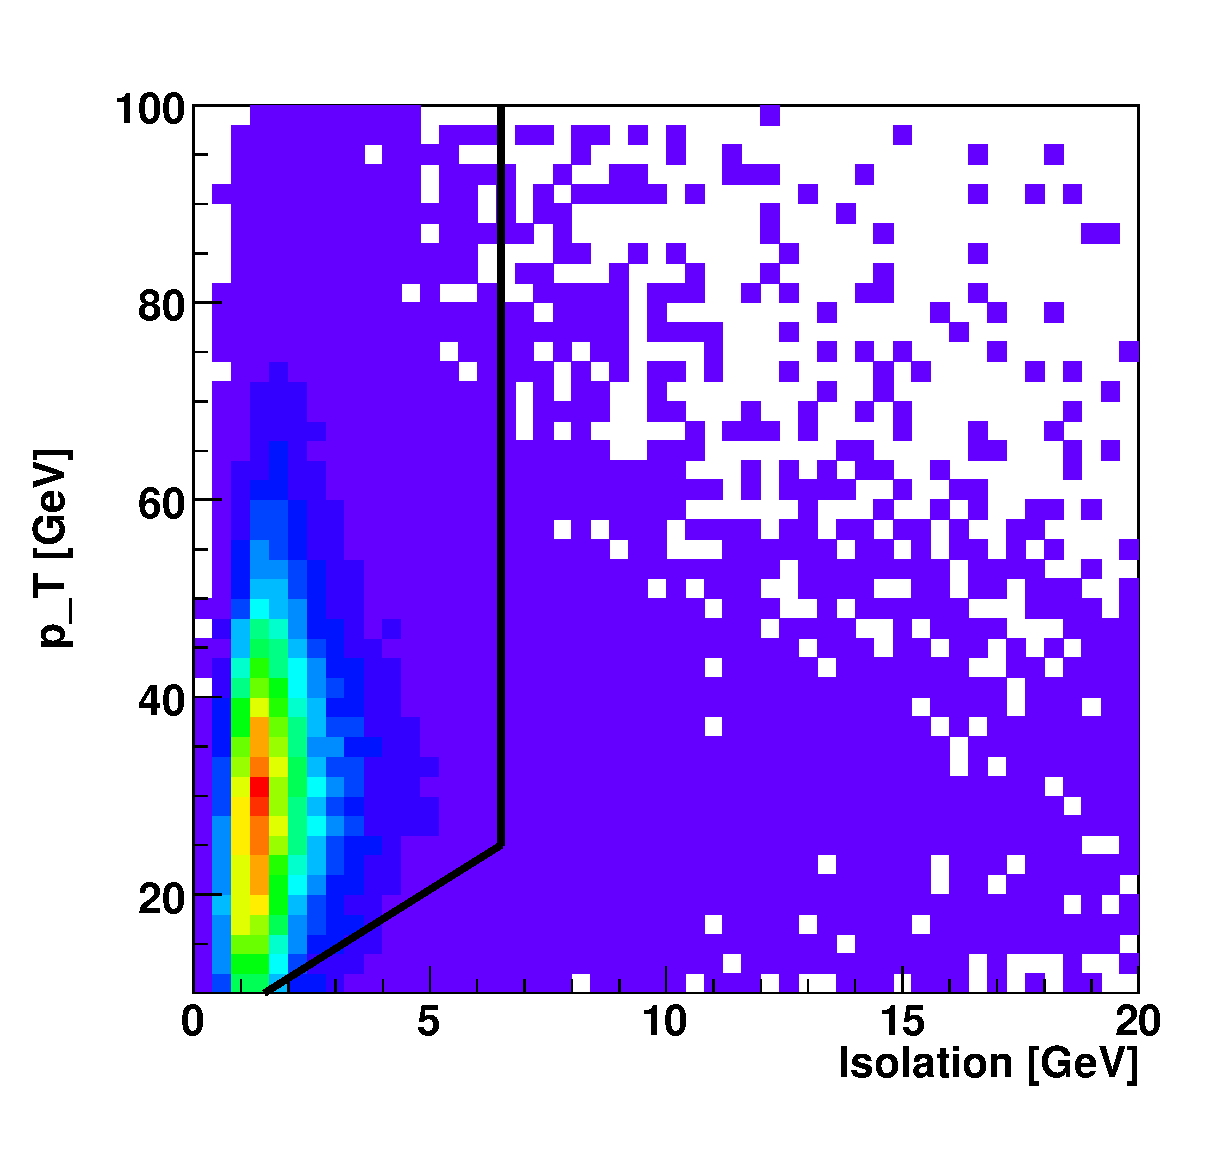
\includegraphics[width=0.49\textwidth]{plots/pt_iso_el_h150ww.eps}} 
    \subfigure[]{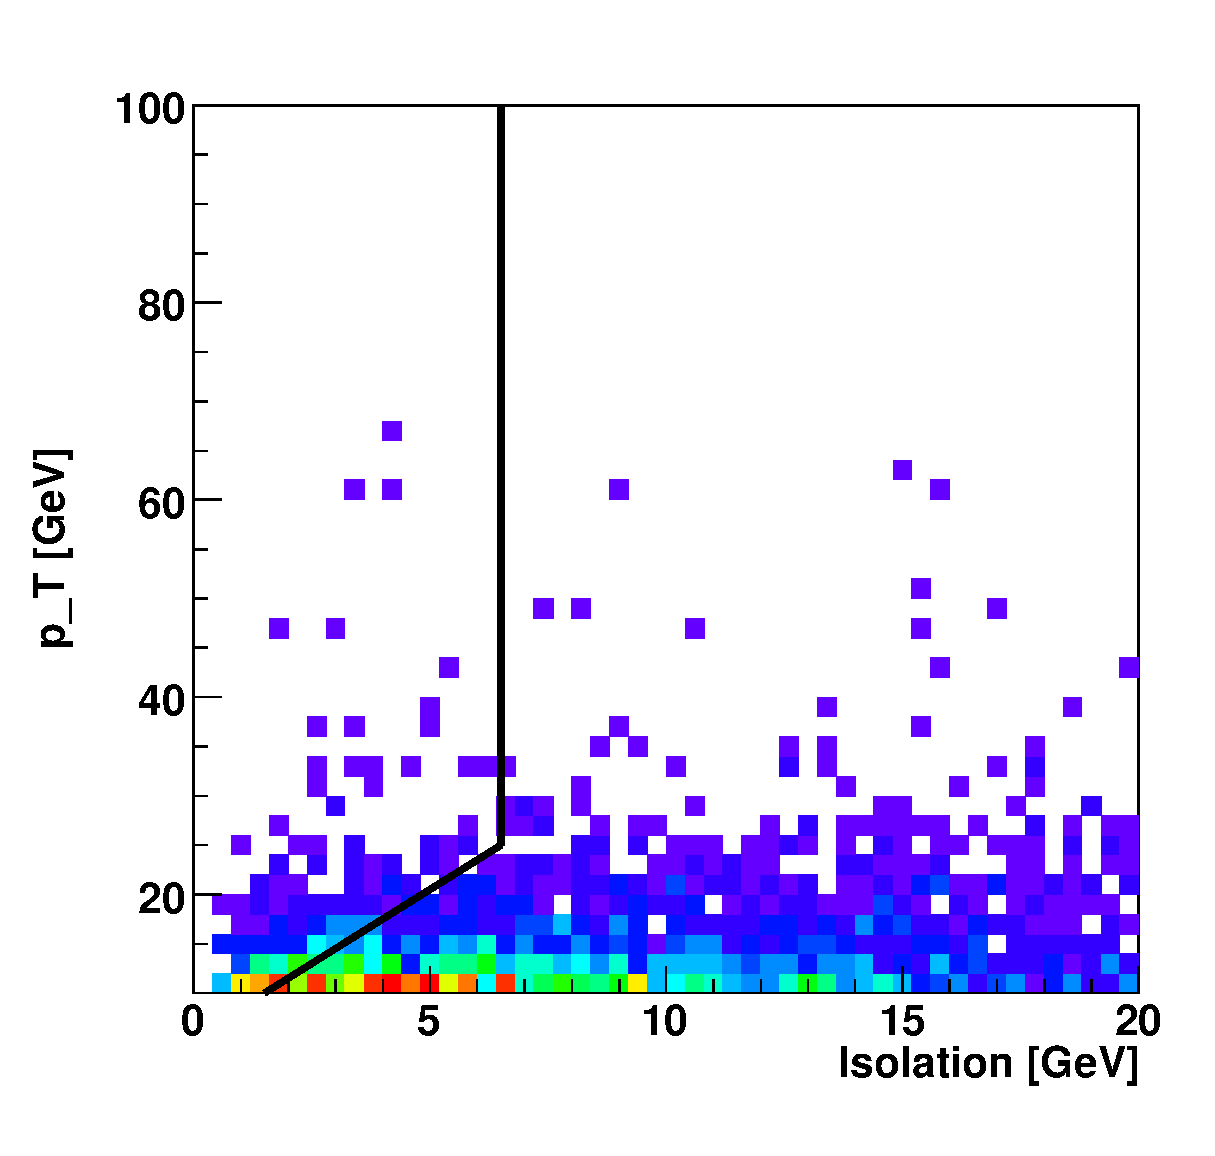
\includegraphics[width=0.49\textwidth]{plots/pt_iso_el_qcd.eps}}
    
    \caption{The two dimensional $p_T$ versus isolation distribution for electrons in (a) \HiggsToWW\ events with a Higgs boson mass of $150$~\GeVcc and (b) QCD events. The black line shows the isolation cut, where everything to the left of the boundary is accepted and everything to the right is rejected.}
    \label{fig:pt_iso_el_h150ww}
  \end{center}
\end{figure}


For the electron denominator we consider two definitions, one looser and one tighter, in order to study the difference in performance.

\begin{enumerate}
\item GsfTrack denominator (looser) : A GsfTrack is matched in direction to a supercluster. We loop over all reconstructed superclusters in the event and search for the GsfTrack whose $E/P$ is closest to one, with the requirement that the $\delta$R to the supercluster is less than 0.3. Any such match found is a denominator if they also satisfy the following requirements:
  \begin{itemize}
  \item $p_T > 10.0$~\GeVc , where the $p_T$ is computed using the energy measurement from the supercluster and the direction from the GsfTrack,
  \item trackIsolation (sumPt of tracks with $p_T > 1.0$~\GeVc~and within a $\Delta$R cone of 0.3) $< 10.0$~\GeVc,
  \item impact parameter cut: $d_{0} < 0.025$~cm, and
  \item conversion veto: a GsfTrack that matches one leg of a well identified conversion is rejected.
  \end{itemize}
 
\item Reco Denominator (tighter): A pixel seeded GSF electron candidate which satisfies the following requirements:
  \begin{itemize}
  \item $p_T > 10.0$~\GeVc, where the $p_T$ is computed using the energy measurement from the supercluster and the direction from the GsfTrack,
  \item trackIsolation (sumPt of tracks with $p_T > 1$~\GeVc~and within a $\Delta$R cone of 0.3) + Jurassic Ecal Isolation $< 10.0$~\GeV,
  \item impact parameter cut: $d_{0} < 0.025$~cm, and
  \item conversion veto: an electron GsfTrack that matches one leg of a well identified conversion is rejected.
  \end{itemize}
\end{enumerate}

\customSubsubsection{Muons}  
Numerator: A Global Muon passing the following cuts~ \cite{muonID}:
\begin{itemize}
\item $p_T > 10.0$~\GeVc,
\item complies with the TMOneStationLoose requirements, which ensures that the track segments measured in the muon chambers are consistent with those generated by a single charged particle,
\item complies with the TM2DCompatibilityLoose requirements, which ensures that the calorimeter energy deposition in the direction of the muon is consistent with a MIP,
\item isolation cut: $\frac{totalIso}{p_T - 10\GeVc} < 0.33$ if $p_T <= 25~\GeVc$, and $totalIso < 5.0~\GeVc$ if $p_T > 25\GeVc$, where $totalIso = trackIso + EcalIso + HcalIso$, and
\item impact parameter cut: $d_{0} < 0.025$~cm.
\end{itemize}

To illustrate the isolation cut, we show the two dimensional $p_T$ versus isolation distributions for a signal and a background sample in \FigureRef{fig:pt_iso_mu_h150ww}.

\begin{figure}[htb]
  \begin{center}
    \subfigure[]{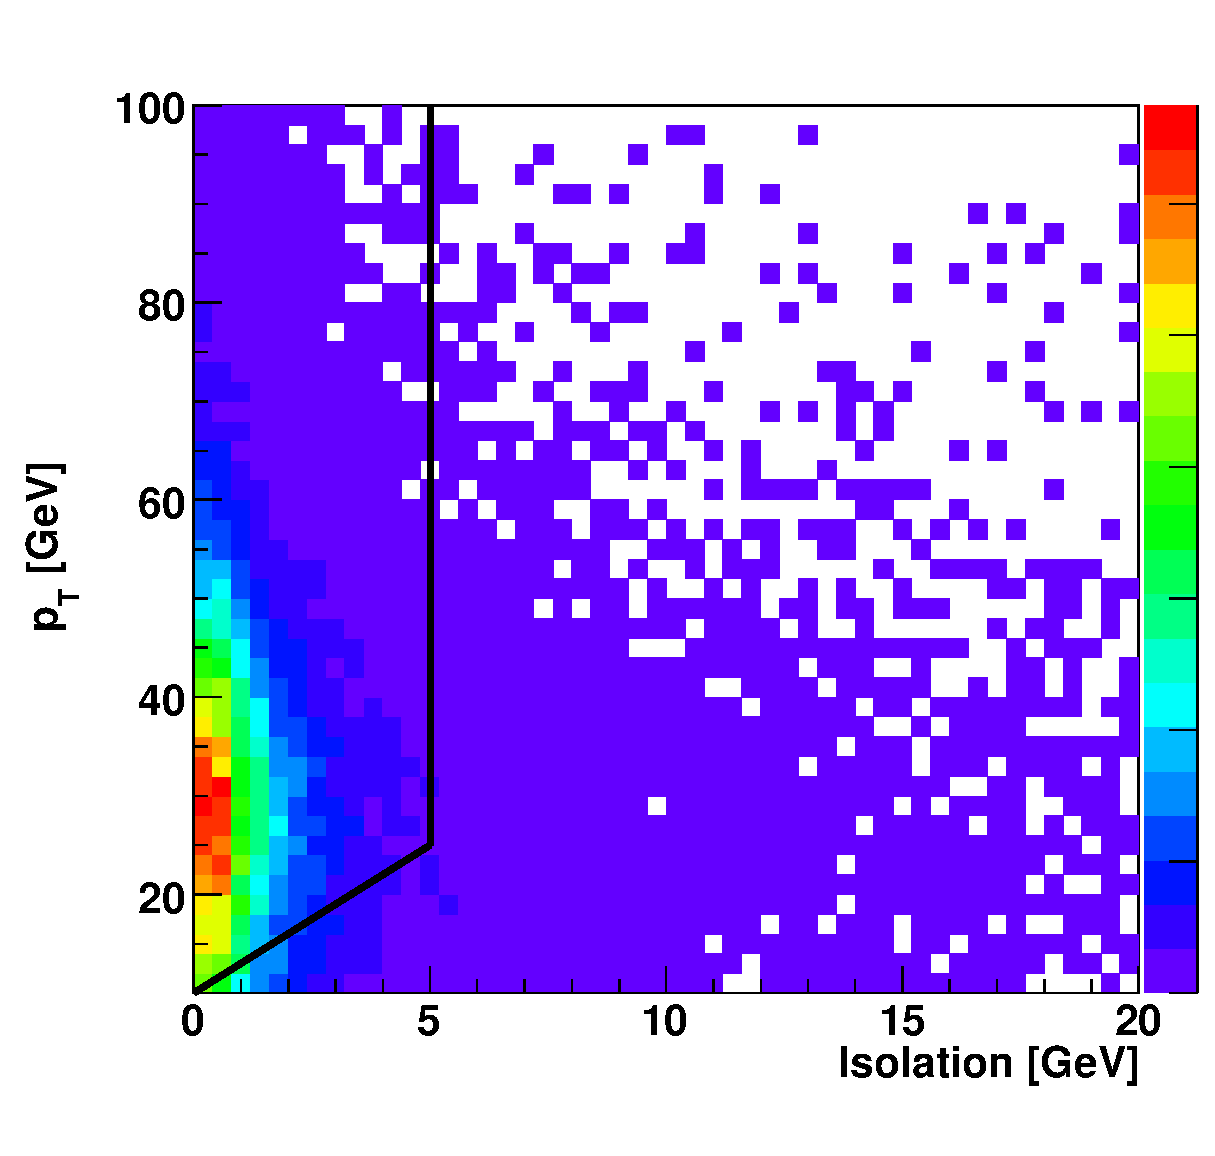
\includegraphics[width=0.49\textwidth]{plots/pt_iso_mu_h150ww.eps}} 
    \subfigure[]{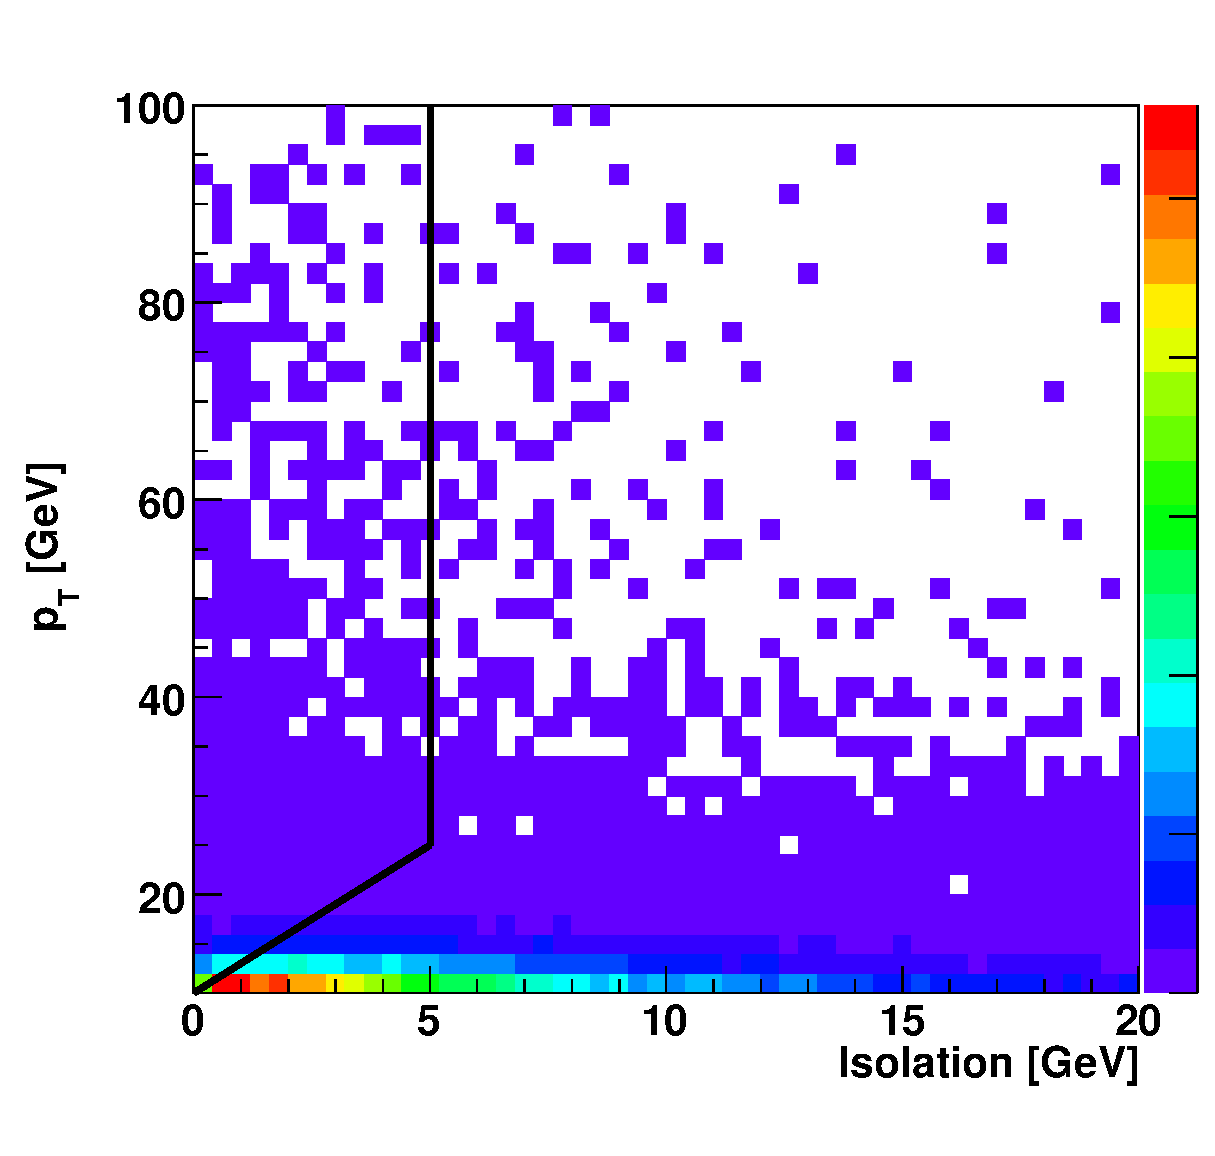
\includegraphics[width=0.49\textwidth]{plots/pt_iso_mu_qcd.eps}}
    
    \caption{The two dimensional $p_T$ versus isolation distribution for muons in (a) \HiggsToWW\ events with a Higgs boson mass of $150~\GeVcc$ and (b) QCD events. The black line shows the isolation cut, where everything to the left of the boundary is accepted and everything to the right is rejected.}
    \label{fig:pt_iso_mu_h150ww}
  \end{center}
\end{figure}

For the muon denominator we consider three definitions, in order to study the difference in performance. They are given in order of increasing tightness.

\begin{enumerate}
\item Isolated track denominator : Any track with track isolation less than $10.0$~\GeVc.
\item Tracker muon denominator : A tracker muon candidate. These are tracks which are matched to a hit in the muon chambers. The isolation requirement is as for the isolated track denominator.
\item Global muon denominator : A global muon candidate. These are muons that pass the global muon fit. The isolation requirement is as for the isolated track denominator.
\end{enumerate}


\customSubsection{Measurement of Fake Rate}
Two samples are proposed for the measurement of the fake rate in data. In the absence of data we use Monte Carlo samples to emulate what one expects the data sample to look like.

\customSubsubsection{Jet Triggered Sample}
\label{sec:jetTriggeredSample}
The first calibration sample are events triggered by jet triggers. Since the dominant high transverse momentum process at the LHC are QCD multijet events, the events which are triggered by the existence of a high energy jet are enhanced for multijet events. The treatment and effect of contamination from \WPM\ and \Z\ events will be discussed in Sections~\ref{sec:signalcontamination_electron} and \SectionRef{sec:signalcontamination_muon}.
.

For this sample we use the Fall08 Madgraph QCD and PhotonJets samples and require that they pass the HLT\_Jet50 trigger. We use version CMSSW\_2\_2\_10 of the software. For a list of triggers in the Summer08 and Fall08 samples see Ref.~\cite{HLTTable}. The samples used are as follows:
\begin{itemize}
\item /QCD100to250-madgraph/Fall08\_IDEAL\_V11\_redigi\_v1/GEN-SIM-RECO,
\item /QCD250to500-madgraph/Fall08\_IDEAL\_V11\_redigi\_v1/GEN-SIM-RECO,
\item /QCD500to1000-madgraph/Fall08\_IDEAL\_V11\_redigi\_v1/GEN-SIM-RECO,
\item /QCD1000toInf-madgraph/Fall08\_IDEAL\_V11\_redigi\_v1/GEN-SIM-RECO,
\item /PhotonJets40to100-madgraph/Fall08\_IDEAL\_V11\_redigi\_v2/GEN-SIM-RECO,
\item /PhotonJets100to200-madgraph/Fall08\_IDEAL\_V11\_redigi\_v2/GEN-SIM-RECO, and 
\item /PhotonJets200toInf-madgraph/Fall08\_IDEAL\_V11\_redigi\_v2/GEN-SIM-RECO.
\end{itemize}

In order to avoid a bias of the fake rate measurement due to particular requirements on the shower shape of a trigger jet, we remove any denominator and numerator event inside of a cone with $\Delta R < 0.3$ around the leading trigger jet, whose size is chosen equal to the cone size used for computing the lepton isolation. 

\customSubsubsection{Photon Triggered Sample}
\label{sec:photonTriggeredSample}
The second calibration sample are events triggered by a high energy photon trigger. These events are predominantly $\gamma$+Jets events. Depending on the strictness of the requirement on the reconstructed photon, QCD multijet events contribute to this sample as well, where the trigger photon is caused by a jet that has fakes the photon. The numerator distribution in this sample will also contain leptonically decaying \WPM\ and \Z\ events which pass the trigger either due to a real photon in the event or due to an electron that fakes a trigger photon. These contributions will be subtracted from the numerator and denominator using the Monte Carlo simulation prediction. This is one example of the second order corrections from Monte Carlo simulation that are required.

For the purpose of modelling the \WPlusJets\ background to two lepton final states, using the photon triggered sample to measure the fake rate is expected to perform better than using the jet triggered sample, due to the fact that the quark to gluon fraction of the jets in the $\gamma$+Jets process is closer to the quark to gluon fraction of jets produced in \WPlusJets\ events. 

For this sample we use the Summer08 Pythia PhotonJets samples and require they pass the HLT\_Photon15 trigger. We require one reconstructed photon which passes the following photon identification cuts and lies within a $\Delta$R cone of 0.3 around the trigger photon\cite{PhotonID}.

\begin{itemize}
\item $p_T > 20.0~\GeVc$,
\item Hadronic energy / Electromagnetic energy $< 0.03$,
\item Photon supercluster was not seeded by pixel hits,
\item Isolation:  track isolation  + hadronic calorimeter isolation $< 5.0$~\GeV, and
\item $R_9 > 0.8$
\end{itemize}

We remove any numerator and denominator event that lies inside of a cone of $\Delta R < 0.3$ around the trigger photon. In order to reduce contamination from QCD multijet events, we make the following cuts:

\begin{itemize}
\item $\Delta\phi$ between the trigger photon and the leading jet $> \pi - 0.2$ \cite{JetEnergyCalibrationWithPhotonJet}
\end{itemize}

The samples used are as follows:
\begin{itemize}
\item /QCD100to250-madgraph/Fall08\_IDEAL\_V11\_redigi\_v1/GEN-SIM-RECO,
\item /QCD250to500-madgraph/Fall08\_IDEAL\_V11\_redigi\_v1/GEN-SIM-RECO,
\item /QCD500to1000-madgraph/Fall08\_IDEAL\_V11\_redigi\_v1/GEN-SIM-RECO,
\item /QCD1000toInf-madgraph/Fall08\_IDEAL\_V11\_redigi\_v1/GEN-SIM-RECO,
\item /PhotonJets40to100-madgraph/Fall08\_IDEAL\_V11\_redigi\_v2/GEN-SIM-RECO,
\item /PhotonJets100to200-madgraph/Fall08\_IDEAL\_V11\_redigi\_v2/GEN-SIM-RECO, and 
\item /PhotonJets200toInf-madgraph/Fall08\_IDEAL\_V11\_redigi\_v2/GEN-SIM-RECO
\end{itemize}


\customSubsection{Application of Fake Rate}
After we have measured the fake rates we apply them in a particular data sample. For simplicity, we will only discuss the case where one lepton in the selected signal sample is a fake. In this case, one takes a sample where the number of well identified leptons is one less than the selected final state (the extrapolation sample). Then one promotes each denominator object to a numerator, one by one, and gives the event a weight equal to the fake rate for that denominator object. Performing this for the entire extrapolation sample gives the prediction for the background to the selected signal sample consisting of one fake lepton. 

Care must be taken to allow all denominator objects in the event to be promoted to a numerator. For example, if there are three denominators in an event ($d_1$, $d_2$, $d_3$) each with fake rates $f_1$, $f_2$, $f_3$, then the prediction must consist of three events: one event where only $d_1$ is a numerator with weight $f_1$, one event where only $d_2$ is a numerator with weight $f_2$, and one event where only $d_3$ is a numerator with weight $f_3$. Furthermore, if one is considering both electron and muon fakes simultaneously, one has to make sure that promoted numerators for electrons and muons do not overlap, ie. they do not come from the same underlying object. 

This method can also be applied to cases where one is interested in more than one fake lepton in the final state. To illustrate by example, if one is interested in predicting the background to the four lepton final state from Z + 2Jets, one takes a sample consisting of a well reconstructed Z boson plus two or more denominator objects. One then promotes two denominators to become numerators with each of their individual fake rates multiplied. If there are more than two denominators in the event, one has to account for all possible combinations. An example of the correct treatment of combinatorics is given in \AppendixRef{app:combinatorics}.

\customSubsubsection{Second order corrections to \epsilonFake}
There are two subtle details for which corrections to the fake rate are necessary. Since we explicitly reject events for which two leptons pass the full lepton identification criteria for the extrapolation sample, we do not count those lepton plus denominator events for which the denominator actually passed the full lepton identification. This contribution needs to be added to the prediction. The final background prediction is given by the following expression:

\begin{eqnarray}
  N^{\textrm{sig}}_{\textrm{two leptons}} & = & N^{\textrm{ext}}_{\textrm{l+d}} \times \epsilonFake \nonumber \\
  & = &  \left(\frac{N^{\textrm{ext}}_{\textrm{l + d fails lepton ID}}}{1-\epsilonFake}\right) \times \epsilonFake  \nonumber \\
  & = &  N^{\textrm{ext}}_{\textrm{l + d fails lepton ID}} \times \left(\frac{\epsilonFake}{1-\epsilonFake}\right)   \nonumber \\
\end{eqnarray}

where, the subscript $\textrm{sig}$ refers to the selected signal sample, $\textrm{ext}$ refers to the extrapolation sample where we have events with one less lepton than the selected final state plus any number of denominators, $\textrm{l}$ refers to the real lepton, $\textrm{f}$ refers to the fake object, and $\textrm{d}$ refers to the denominator object. $N^{ext}_{\textrm{l + d fails lepton ID}}$ is the number measured in the extrapolation sample, and $N^{ext}_{\textrm{l+d}}$ is the total number of lepton plus denominator events regardless of whether the denominator passed or failed lepton identification. The relation $N^{ext}_{\textrm{l + d fails lepton ID}} = (1-\epsilonFake) \times N^{ext}_{\textrm{l+d}}$ is used.

There is a further correction due to the fact that in the signal region there are events for which the real lepton failed to fire the trigger while the fake lepton fired the trigger. These events are generally not included in the extrapolation sample since the probability that only the denominator object fires the trigger is small. A small correction factor must be applied.

The correction is obtained by using the Monte Carlo simulation to obtain the ratio of events for which the real lepton fired the trigger to the events for which the real lepton did not fire the trigger. 
%% \begin{eqnarray}
%% \frac{N^{\textrm{sig}}_{\textrm{l fails HLT \& f fires HLT}}}{N^{\textrm{sig}}_{\textrm{HLT fired}}} & = &  \frac{N^{\textrm{MC\ sig}}_{\textrm{l fails HLT \& f fires HLT}}}{N^{\textrm{MC\ sig}}_{\textrm{HLT fired}}} \nonumber \\
%% \end{eqnarray}
Another implicit assumption is made:
\begin{eqnarray}
N^{\textrm{ext}}_{\textrm{HLT fired}} = N^{\textrm{ext}}_{\textrm{l fires HLT}} + N^{\textrm{ext}}_{\textrm{l fails HLT \& d fires HLT}} & \approx & N^{\textrm{ext}}_{\textrm{l fires HLT}} \nonumber \\
\end{eqnarray}
This assumption is true if \epsilonFake~ is small because then the probability that the real lepton fails the HLT and the denominator passes the HLT is small.

With those assumptions, the prediction for the selected signal sample is given as follows:

\begin{eqnarray}
  N^{\textrm{sig}}_{\textrm{HLT fired}} & = & N^{\textrm{sig}}_{\textrm{l fires HLT}} + N^{\textrm{sig}}_{\textrm{l fails HLT \& f fires HLT}} \nonumber \\
  & \approx &  N^{\textrm{ext}}_{\textrm{HLT fired}} \frac{\epsilonFake}{1-\epsilonFake} +  N^{\textrm{ext}}_{\textrm{HLT fired}} \frac{N^{\textrm{MC\ sig}}_{\textrm{l fails HLT \& f fires HLT}}}{N^{MC\ sig}_{\textrm{HLT fired}}} \frac{\epsilonFake}{1-\epsilonFake} \nonumber \\
  & = &  N^{\textrm{ext}}_{\textrm{HLT fired}} \left(1+R_{MC}\right) \frac{\epsilonFake}{1-\epsilonFake} \nonumber \\
\end{eqnarray}

where $R_{\textrm{MC}} = N^{\textrm{MC}}_{\textrm{l fails HLT \& fake passes HLT}} / N^{\textrm{MC}}_{\textrm{at least one of l or fake passes HLT}}$, and \epsilonFake~ is the fake rate measured in the orthogonal fake enhanced sample. The above correction is adequate only for sufficiently loose denominator definitions. For denominator definitions that are very close to the numerator definition, the correction is not needed (see \AppendixRef{app:triggerCorrection}).

These corrections are typically on the order of $10\%$ of the measured values of \epsilonFake. Therefore, the inaccuracy of the assumptions are not expected to yield large uncertainties on the prediction. Even if the Monte Carlo simulation estimates this correction wrongly by $50\%$, it would only yield an uncertainty of $5\%$ on the final prediction.

\customSection{Results Using Monte Carlo Simulation}
We present results of the fake rate measurement in Monte Carlo simulation. The measured fake rate is used to predict the fake lepton background to the two lepton final state, and compared with the Monte Carlo simulation prediction for the \WPlusJets\ process. All results shown assume an integrated luminosity of $200\ipb$. Finally we discuss studies of systematic uncertainties of this approach. 


\customSubsection{Electron Fake Rates from Monte Carlo}
\label{sec:electronfakerates}
Using the methods described above, we measure the fake rate for both electron denominator definitions parameterized in bins of $p_T$ and $\eta$. A few one-dimensional $\eta$ and $p_T$ slices of the fake rates, as well as the full two dimensional fake rate table are given in \AppendixRef{app:electronfakerates}. The electron fake rate generally rises versus $p_T$ in the low $p_T$ region, and is generally larger at large $\eta$ and lower in the central region of the detector. This is due to increased conversion probability due to more material and worse detector performance in the endcap.

For ease of display, in this section we show one-dimensional projections of the fake rate. The comparison of the electron fake rates computed in the different samples are shown in \FigureRef{fig:electronFakeRate_GsfTrack} for the GsfTrack denominator and in \FigureRef{fig:electronFakeRate_Reco} for the Reco denominator. There is a fairly good agreement between the fake rates measured in the jet triggered sample, the photon triggered sample, and the \WPlusJets\ sample. This suggests that applying the fake rates on the \WPlusJets\ sample will yield reasonable predictions. 

\begin{figure}[htb]
  \begin{center}
    \subfigure[]{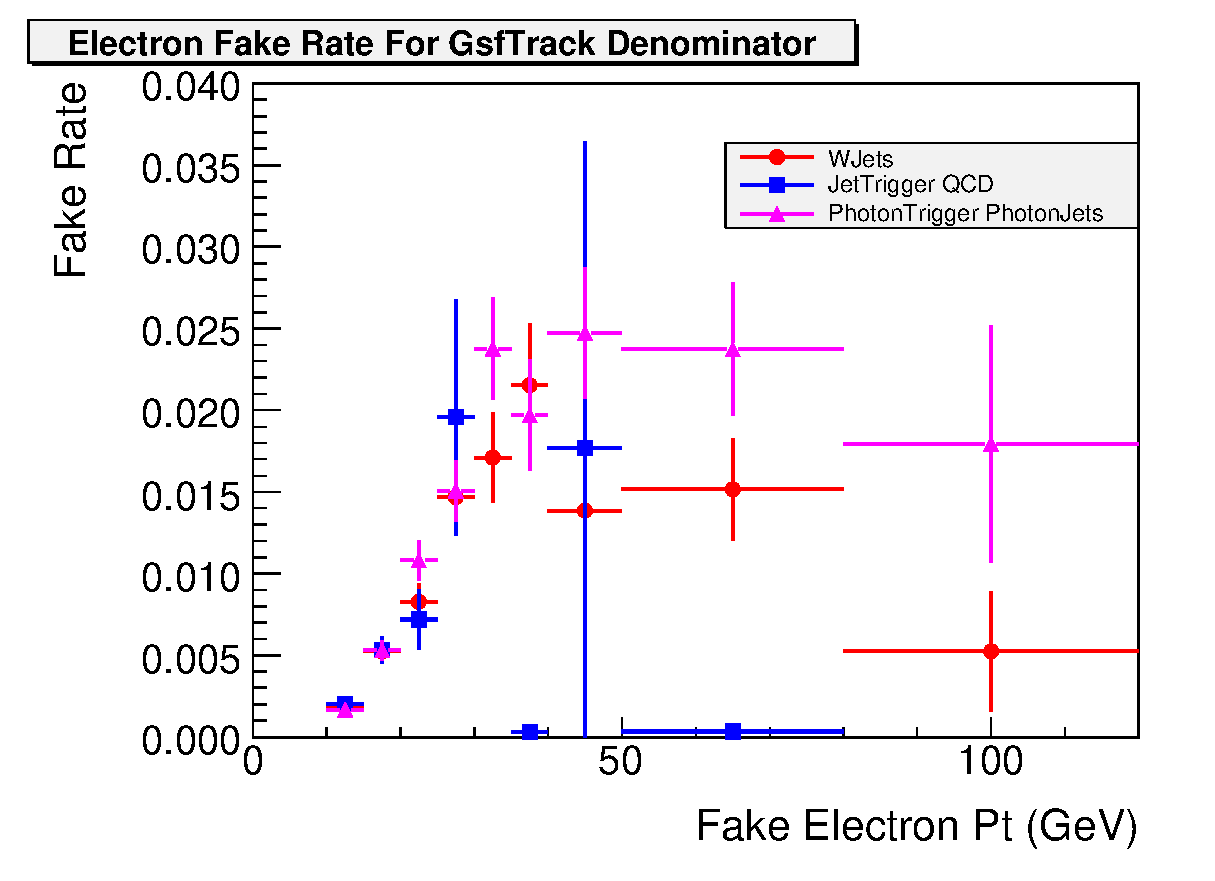
\includegraphics[width=0.49\textwidth]{plots/GsfTrackElectronFakeRatePt.eps}} 
    \subfigure[]{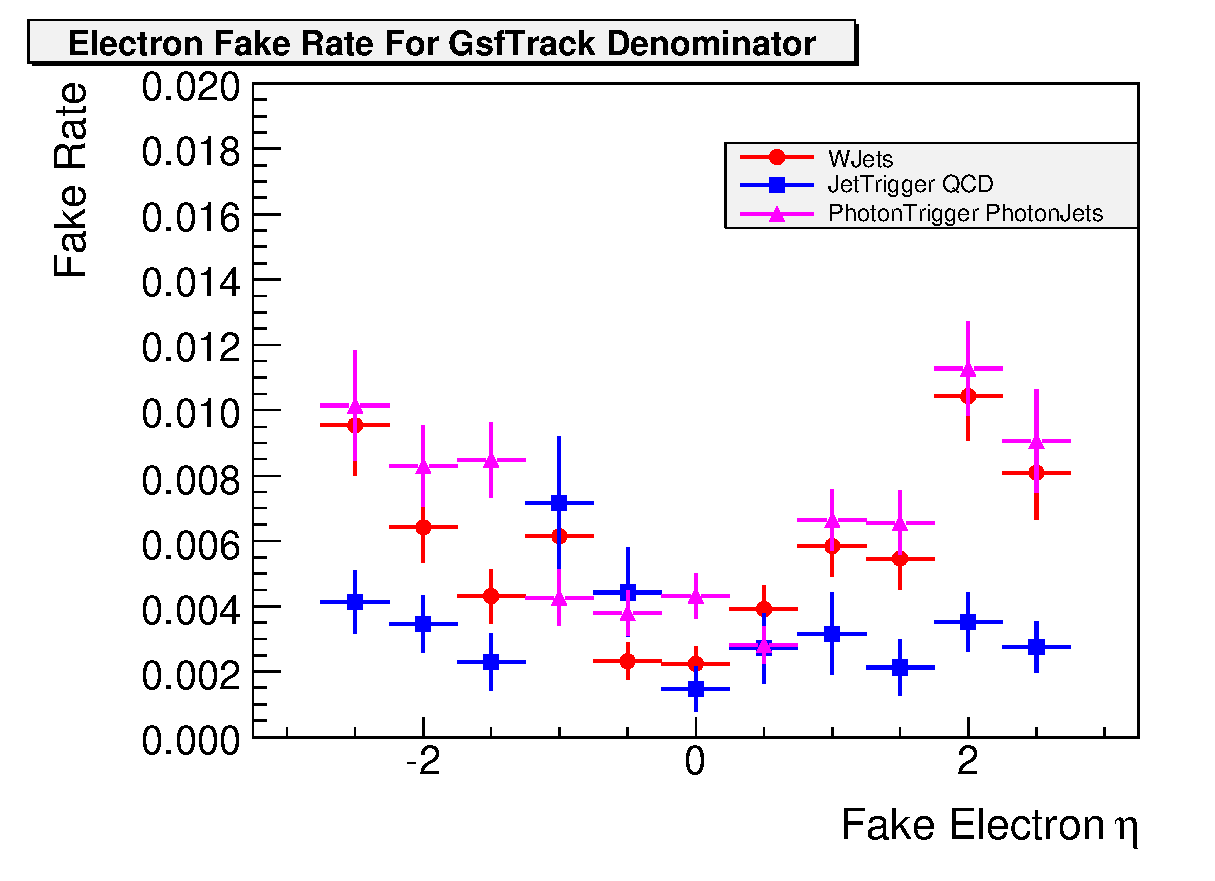
\includegraphics[width=0.49\textwidth]{plots/GsfTrackElectronFakeRateEta.eps}}
    
    \caption{The electron fake rate for the GsfTrack Denominator as a function of the fake electron $p_T$ in (a) and $\eta$ in (b). The points in red circles represent the \epsilonFake measurement using the W+Jets sample, the points in blue squares represent the \epsilonFake measurement using the jet triggered sample, and the points in magenta triangles represent the \epsilonFake measurement using the photon triggered sample.}
    \label{fig:electronFakeRate_GsfTrack}
  \end{center}
\end{figure}

\begin{figure}[htb]
  \begin{center}
    \subfigure[]{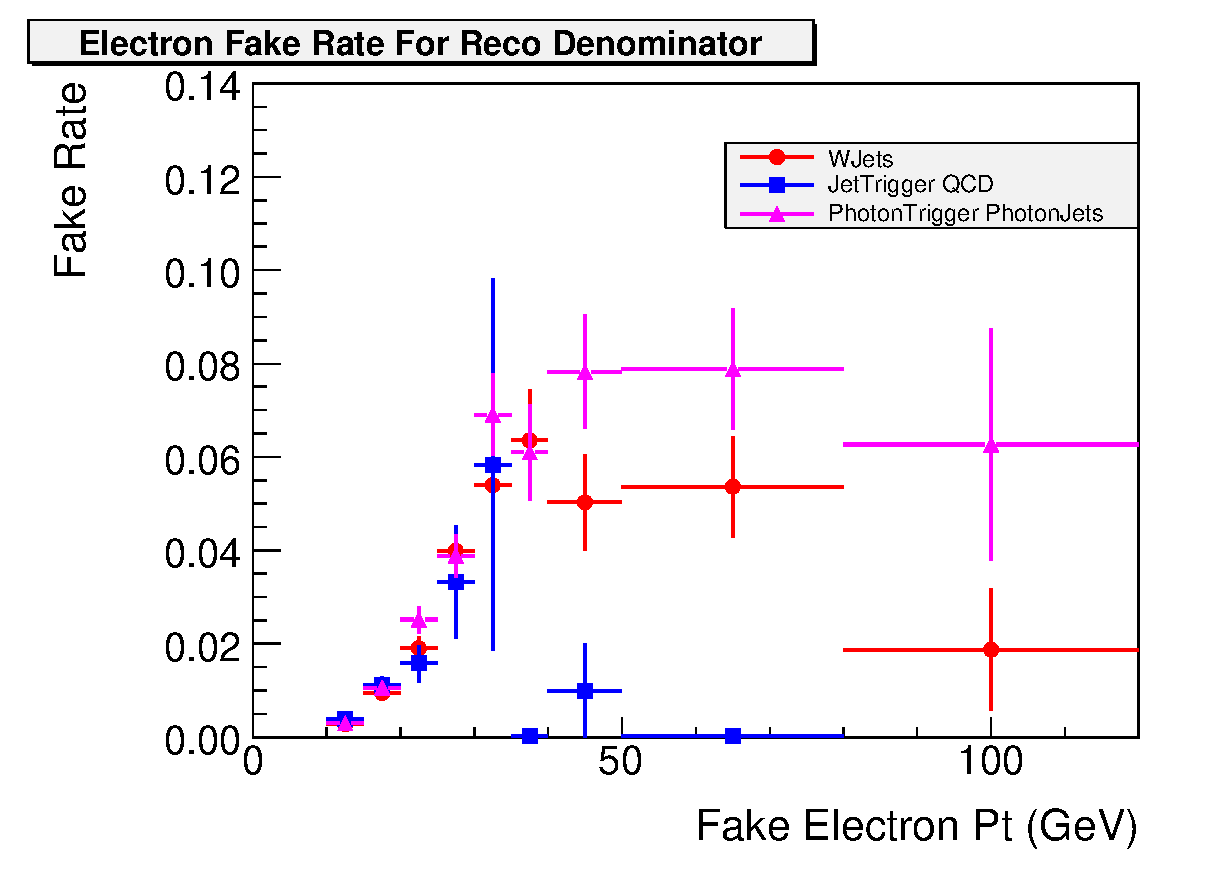
\includegraphics[width=0.49\textwidth]{plots/RecoElectronFakeRatePt.eps}} 
    \subfigure[]{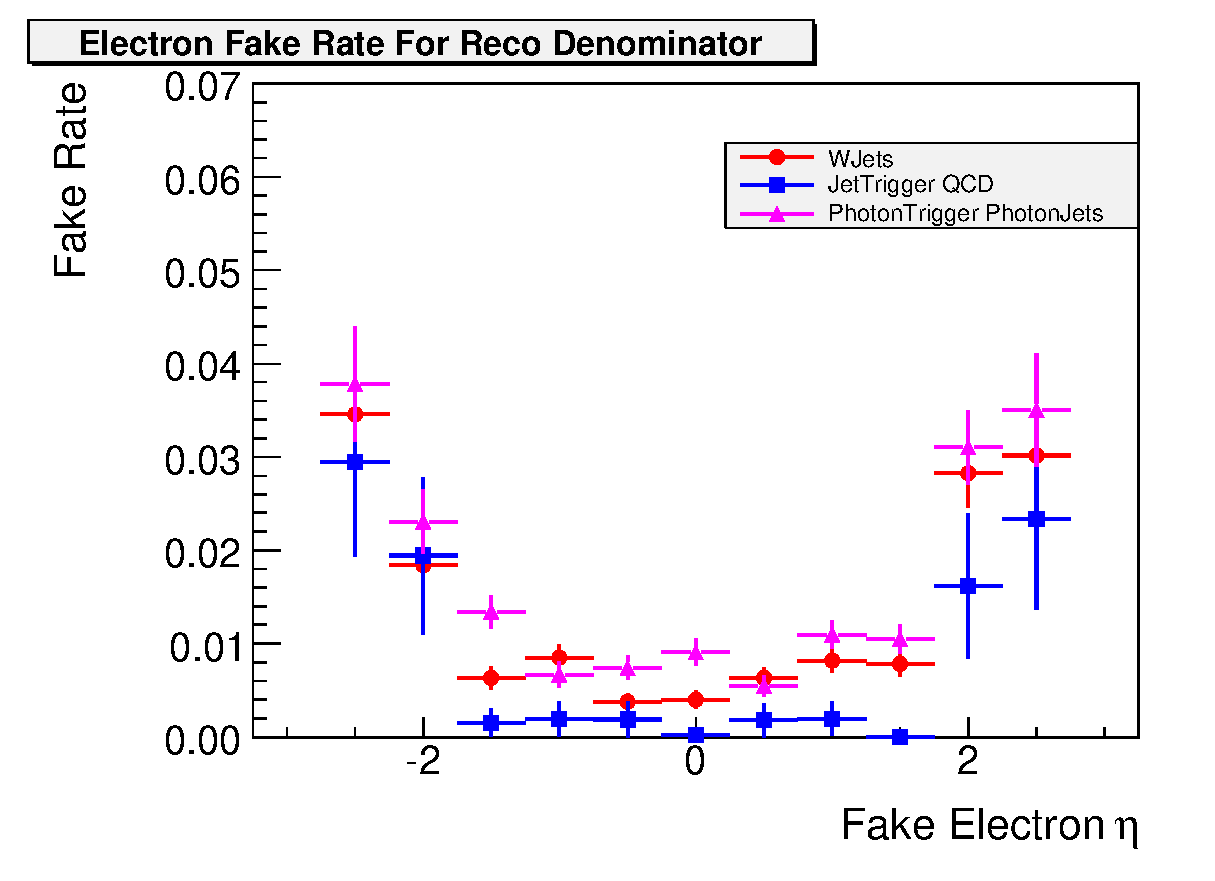
\includegraphics[width=0.49\textwidth]{plots/RecoElectronFakeRateEta.eps}}
    
    \caption{The electron fake rate for the Reco Denominator as a function of the fake electron $p_T$ in (a) and $\eta$ in (b). The color  scheme is as in \FigureRef{fig:electronFakeRate_GsfTrack}.}
    \label{fig:electronFakeRate_Reco}
  \end{center}
\end{figure}

\customSubsubsection{Signal Contamination in the Calibration Sample}
\label{sec:signalcontamination_electron}
In both the jet triggered sample and the photon triggered sample, there are contributions from real isolated leptons to the numerator and denominator distributions. These events include leptonically decaying \WPM\ and \Z\ events that fired the jet or photon triggers. The presence of these objects in the numerator and denominator distributions will bias the fake rate measurement towards larger fake rates because the efficiency for denominators to pass numerator cuts are larger for real leptons. One way to reduce this bias is to use the Monte Carlo simulation to predict the distributions and subtract them from the distributions obtained in data. 

\begin{figure}[htb]
  \begin{center}
    \subfigure[]{\includegraphics[width=0.49\textwidth]{plots/ElectronNumeratorPtStacked_JetTriggerSample_PythiaSeparate.eps}} 
    \subfigure[]{\includegraphics[width=0.49\textwidth]{plots/RecoElectronDenominatorPtStacked_JetTriggerSample_logY_PythiaSeparate.eps}}
    
    \caption{The $p_T$ distribution of the electron numerator (a) and Reco denominator (b) for the jet triggered sample (HLT\_Jet50), showing the contribution from all the relevent physics processes.}
    \label{fig:electronNumeratorDenominatorStacked_JetTriggeredSampleSeparate}
  \end{center}
\end{figure}


\begin{figure}[htb]
  \begin{center}
    \subfigure[]{\includegraphics[width=0.49\textwidth]{plots/ElectronNumeratorPtStacked_PhotonTriggerSample_PythiaSeparate.eps}} 
    \subfigure[]{\includegraphics[width=0.49\textwidth]{plots/RecoElectronDenominatorPtStacked_PhotonTriggerSample_logY_PythiaSeparate.eps}}
    
    \caption{The $p_T$ distribution of the electron numerator (a) and Reco denominator (b) for the photon triggered sample (HLT\_Photon15), showing the contribution from all the relevent physics processes.}
    \label{fig:electronNumeratorDenominatorStacked_PhotonTriggeredSampleSeparate}
  \end{center}
\end{figure}

In Figures~\ref{fig:electronNumeratorDenominatorStacked_JetTriggeredSampleSeparate} and \ref{fig:electronNumeratorDenominatorStacked_PhotonTriggeredSampleSeparate} we show the $p_T$ distributions for the numerator and the Reco denominator in the jet triggered sample and photon triggered sample, separated into the different physics processes. Due to the fact that the Fall08 Madgraph samples do not have full coverage in \ptHat~to show the correct signal to background ratio, these plots are made using the Pythia Summer08 samples:

\begin{itemize}
\item /QCDpt15/Summer08\_IDEAL\_V11\_redigi\_v3/GEN-SIM-RECO,
\item /QCDpt30/Summer08\_IDEAL\_V11\_redigi\_v1/GEN-SIM-RECO,
\item /QCDpt80/Summer08\_IDEAL\_V11\_redigi\_v1/GEN-SIM-RECO,
\item /QCDpt170/Summer08\_IDEAL\_V11\_redigi\_v1/GEN-SIM-RECO,
\item /PhotonJetPt15/Summer08\_IDEAL\_V12\_redigi\_v1/GEN-SIM-RECO,
\item /PhotonJetPt30/Summer08\_IDEAL\_V12\_redigi\_v1/GEN-SIM-RECO,
\item /PhotonJetPt80/Summer08\_IDEAL\_V12\_redigi\_v1/GEN-SIM-RECO, and
\item /PhotonJetPt170/Summer08\_IDEAL\_V12\_redigi\_v1/GEN-SIM-RECO.
\end{itemize}

One sees a non-negligible contribution from \WPM, \Z, and \TTBAR\ events. The unphysical spikes in various bins are due to large weight contributions from Monte Carlo samples with a limited number of events. For the fake rates presented above and used for the prediction, the contamination from \WPM, \Z, and \TTBAR\ events have not been included. The $\gamma$+Jets events were included because they are not expected to be well modelled by simulation and therefore are more difficult to subtract.

\customSubsection{Muon Fake Rates from Monte Carlo}
The muon fake rate is measured for all three denominator definitions parameterized in crude bins in $p_T$ and $\eta$. A few one-dimensional $\eta$ and $p_T$ slices of the fake rates , as well as the full two dimensional fake 
rate table are given in \AppendixRef{appendix:muonfakerates}. The muon fake rates show similar qualitative behaviour as the electron fake rates. 
 
\begin{figure}[htb]
  \begin{center}
    \subfigure[]{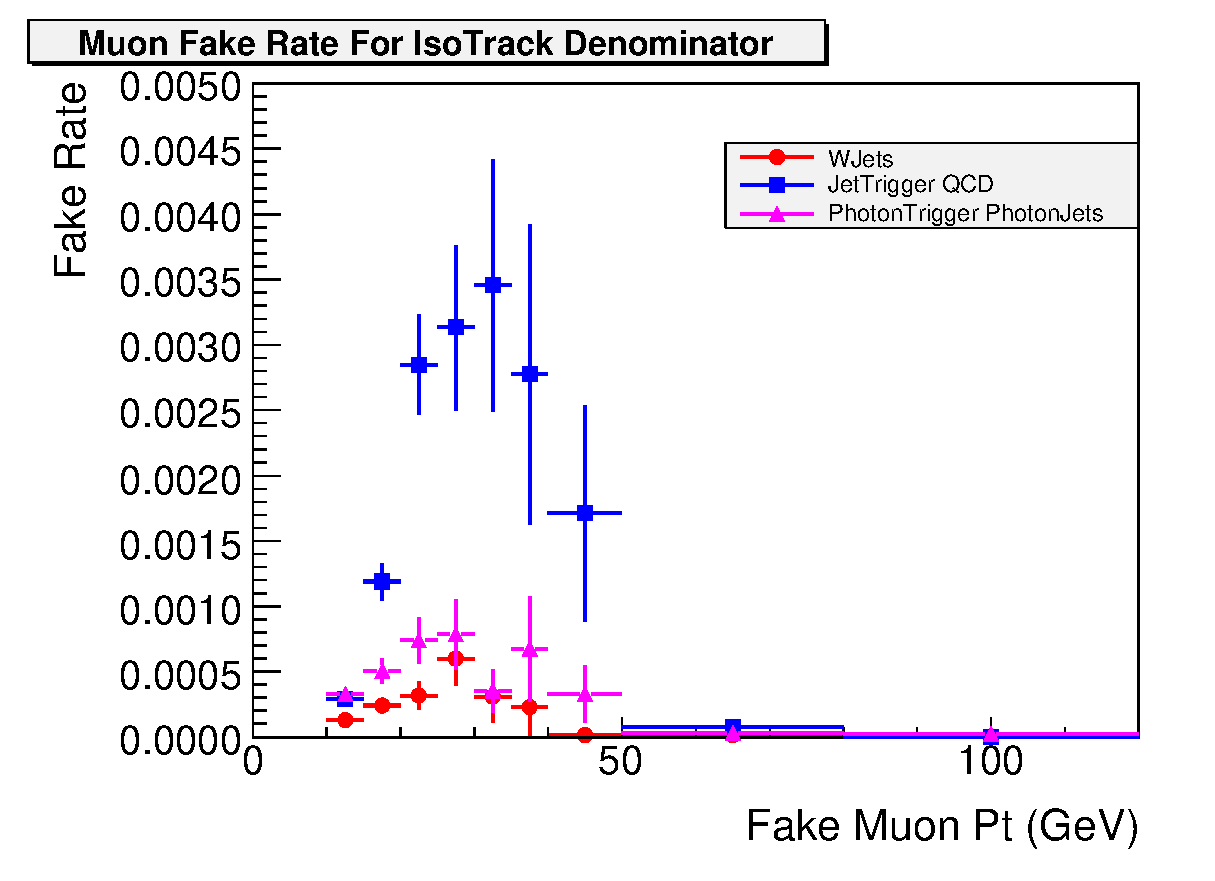
\includegraphics[width=0.49\textwidth]{plots/IsoTrackMuonFakeRatePt.eps}} 
    \subfigure[]{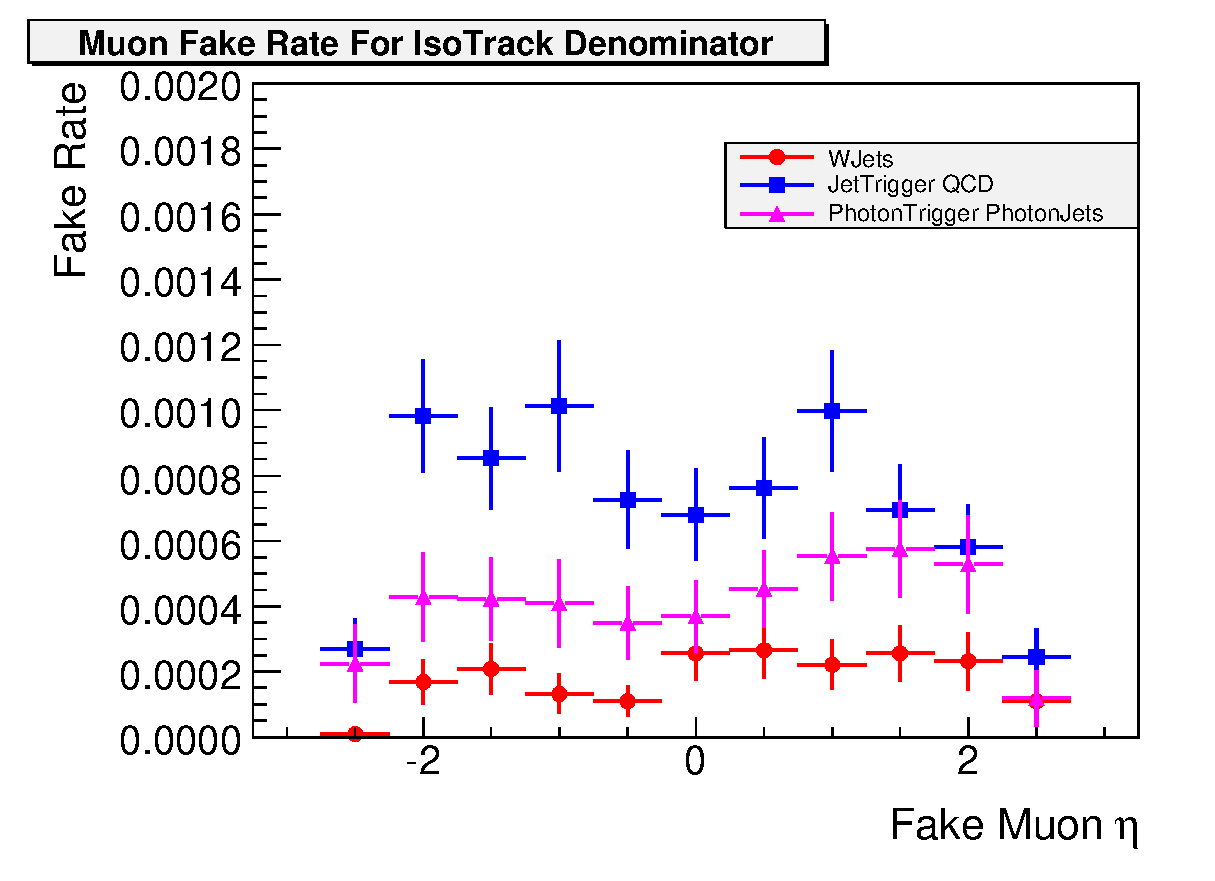
\includegraphics[width=0.49\textwidth]{plots/IsoTrackMuonFakeRateEta.eps}}
    
    \caption{The muon fake rate for the isolated track denominator as a function of the fake muon $p_T$ in (a) and $\eta$ in (b). The color  scheme is as in \FigureRef{fig:electronFakeRate_GsfTrack}.}
    \label{fig:muonFakeRate_IsoTrack}
  \end{center}
\end{figure}

\begin{figure}[htb]
  \begin{center}
    \subfigure[]{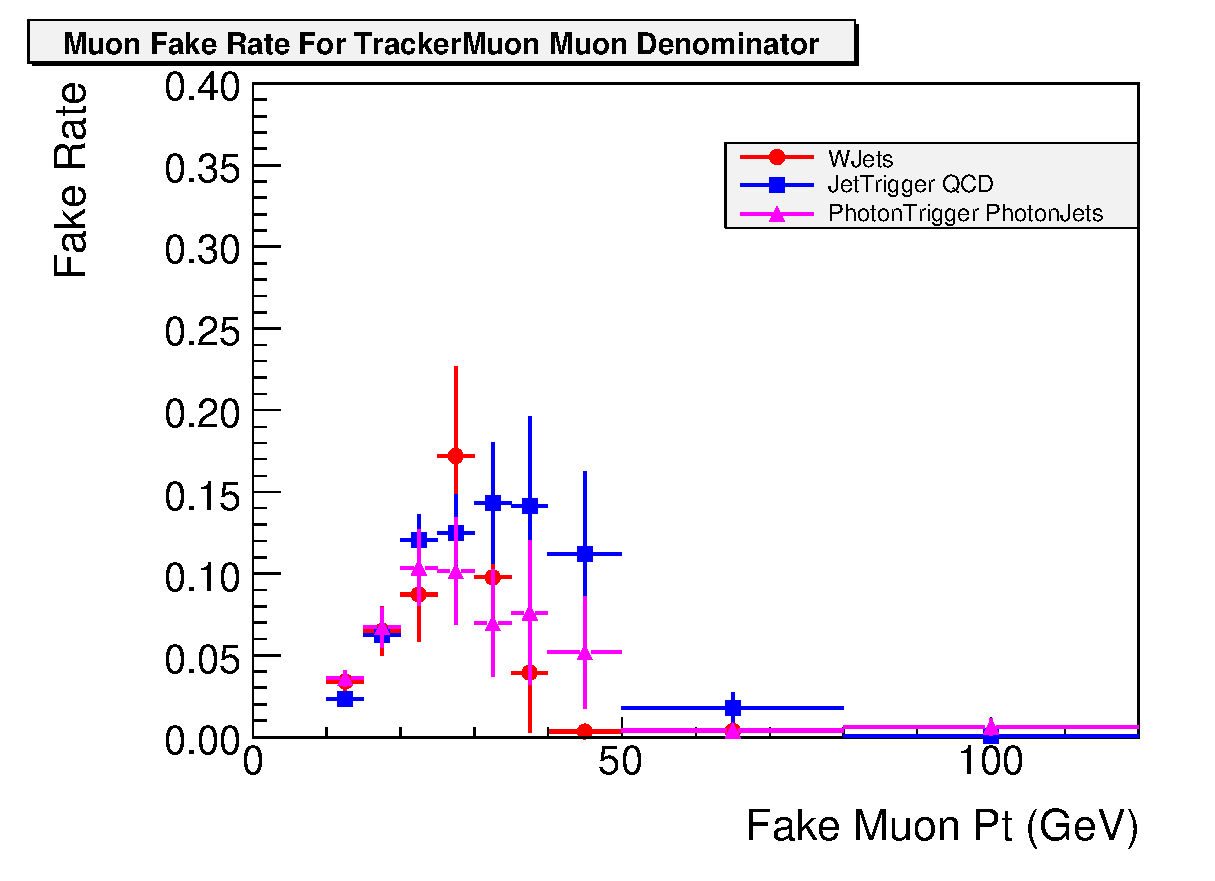
\includegraphics[width=0.49\textwidth]{plots/TrackerMuonFakeRatePt.eps}} 
    \subfigure[]{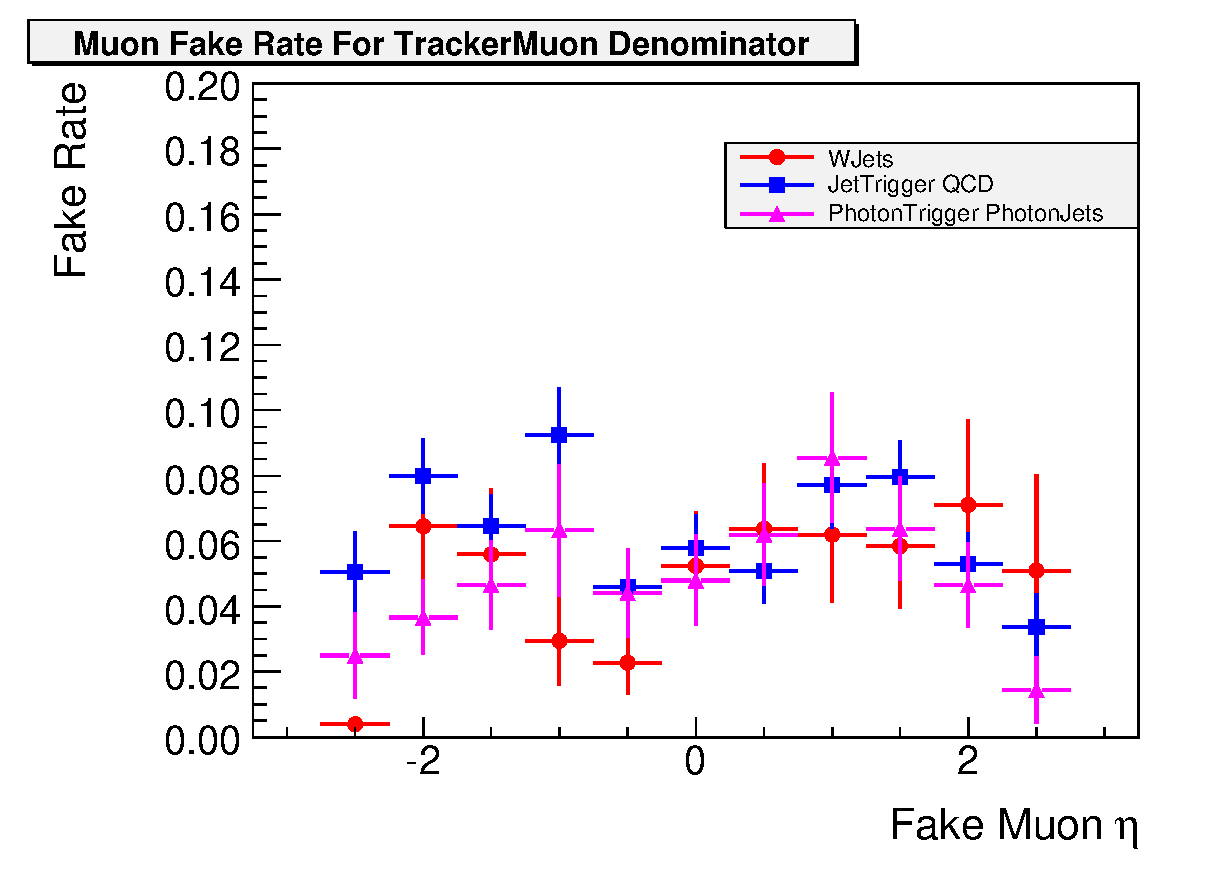
\includegraphics[width=0.49\textwidth]{plots/TrackerMuonFakeRateEta.eps}}
    
    \caption{The muon fake rate for the tracker muon denominator as a function of the fake muon $p_T$ in (a) and $\eta$ in (b). The color  scheme is as in \FigureRef{fig:electronFakeRate_GsfTrack}.}
    \label{fig:muonFakeRate_TrackerMuon}
  \end{center}
\end{figure}

\begin{figure}[htb]
  \begin{center}
    \subfigure[]{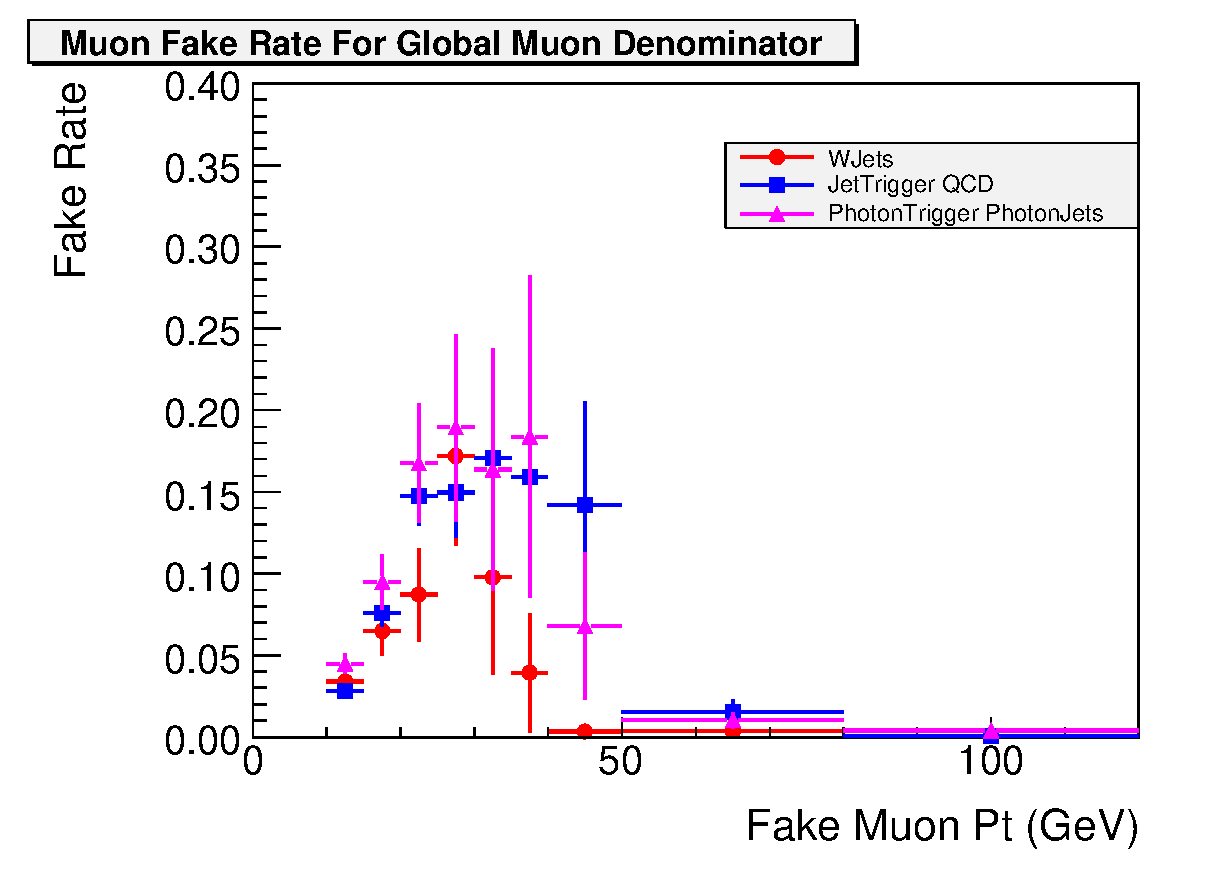
\includegraphics[width=0.49\textwidth]{plots/GlobalMuonFakeRatePt.eps}} 
    \subfigure[]{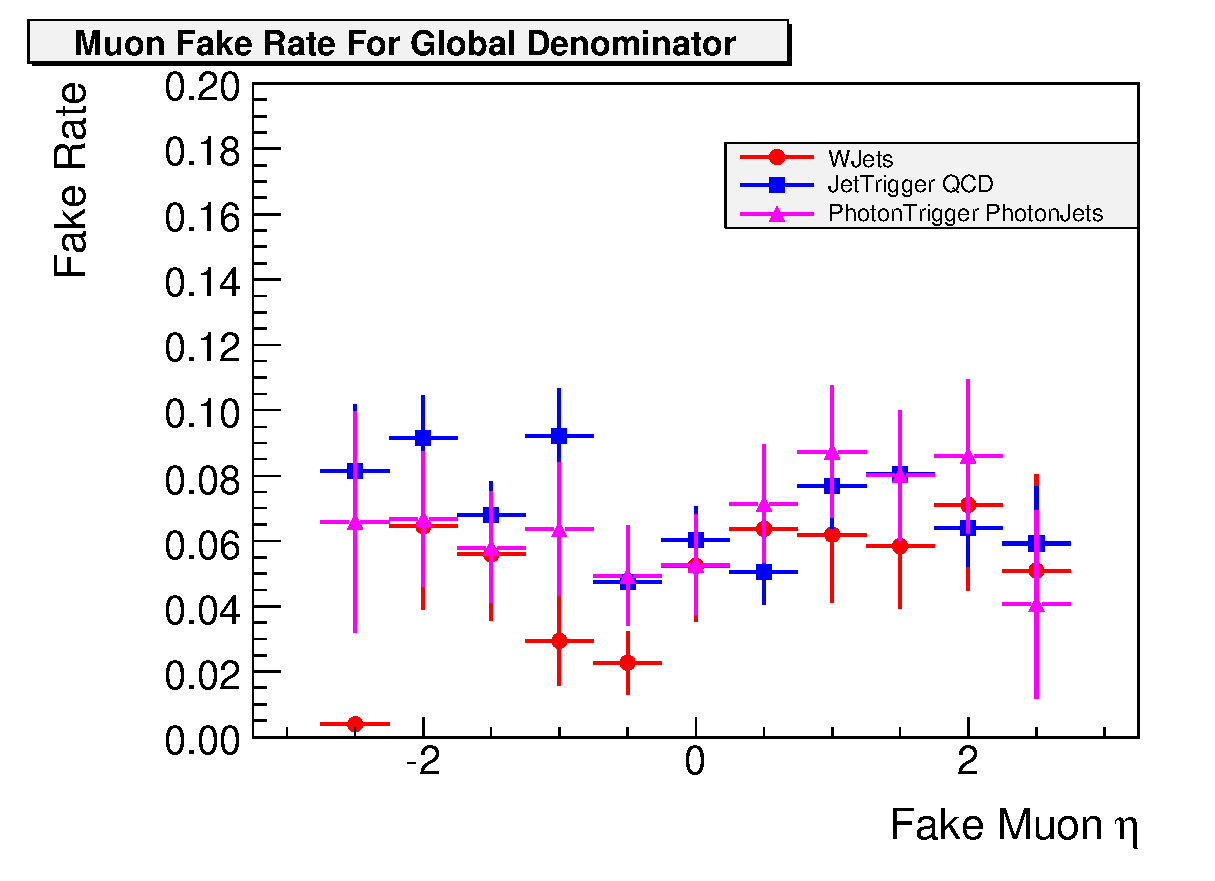
\includegraphics[width=0.49\textwidth]{plots/GlobalMuonFakeRateEta.eps}}
    
    \caption{The muon fake rate for the global muon denominator as a function of the fake muon $p_T$ in (a) and fake electron $\eta$ in (b). The color  scheme is as in \FigureRef{fig:electronFakeRate_GsfTrack}.}
    \label{fig:muonFakeRate_GlobalMuon}
  \end{center}
\end{figure}


For ease of display, we show one-dimensional projections of the fake rate. The comparison of the electron fake rates computed in the different calibration samples are shown in \FigureRef{fig:muonFakeRate_IsoTrack} for the isolated track denominator, in \FigureRef{fig:muonFakeRate_TrackerMuon} for the tracker muon denominator, and in \FigureRef{fig:muonFakeRate_GlobalMuon} for the global muon denominator. For the isolated track denominator we find that the fake rate computed from the JetTriggered QCD sample is significantly larger than the one computed from the \WPlusJets\ sample. This is almost entirely due to larger fraction of heavy flavor semileptonic decays in the QCD sample relative to the \WPlusJets\ sample. The fake rate from the photon triggered sample are in better agreement with the \WPlusJets\ fake rate. For the tracker muon denominator and the global muon denominator, we see a reasonable agreement for both calibration samples. In summary, we conclude that the tracker muon denominator is the most reasonable definition to use, because its performance is as good as the tighter global muon definition and it is expected to yield smaller statistical errors.

\customSubsubsection{Signal Contamination in the Calibration Sample}
\label{sec:signalcontamination_muon}

For the muon fake rate measurement, we also suffer from a real lepton contamination problem. In Figures~\ref{fig:muonNumeratorDenominatorStacked_JetTriggeredSampleSeparate} and \ref{fig:muonNumeratorDenominatorStacked_PhotonTriggeredSampleSeparate} we show the numerator and global muon denominator distributions for the jet triggered sample and photon triggered sample, separated into the different physics processes. Again there is a significant contamination from \WPM\ and \Z\ events, which needs to be subtracted. Similar to the plot for electrons there are several unphysical spikes due to large weight contributions.

\begin{figure}[htb]
  \begin{center}
    \subfigure[]{\includegraphics[width=0.49\textwidth]{plots/MuonNumeratorPtStacked_JetTriggerSample_PythiaSeparate.eps}} 
    \subfigure[]{\includegraphics[width=0.49\textwidth]{plots/GlobalMuonDenominatorPtStacked_JetTriggerSample_logY_PythiaSeparate.eps}}
    
    \caption{The $p_T$ distribution of the muon numerator (a) and global muon denominator (b) for the jet triggered sample, showing the contribution from all the relevent physics processes.}
    \label{fig:muonNumeratorDenominatorStacked_JetTriggeredSampleSeparate}
  \end{center}
\end{figure}


\begin{figure}[htb]
  \begin{center}
    \subfigure[]{\includegraphics[width=0.49\textwidth]{plots/MuonNumeratorPtStacked_PhotonTriggerSample_PythiaSeparate.eps}} 
    \subfigure[]{\includegraphics[width=0.49\textwidth]{plots/GlobalMuonDenominatorPtStacked_PhotonTriggerSample_logY_PythiaSeparate.eps}}
    
    \caption{The $p_T$ distribution of the muon numerator (a) and global muon denominator (b) for the photon triggered sample, showing the contribution from all the relevent physics processes.}
    \label{fig:muonNumeratorDenominatorStacked_PhotonTriggeredSampleSeparate}
  \end{center}
\end{figure}

\customSection{Detailed Fake Composition Studies In Simulation}
The method presented here is affected by a number of systematic effects mainly due to a limited knowledge of the sample composition. Since one extrapolates from the fake-enriched jet sample to the signal region, one implicitly makes the assumption that the fake rate and hence the composition is identical in both samples. This is probably not true. We discuss some effects that have been studied in Monte Carlo simulation which allows us to gain greater understanding on the differences in the fake composition of these two samples. The algorithm which determines the underlying fake process, described in \SectionRef{sec:categorization_algorithm}, has been used for this study.

\clearpage

\customSubsection{Fake Electron Studies}
\customSubsubsection{Fake Electron Categories}

We begin by studying the composition of electron fakes in simulation. \FigureRef{fig:ElectronNumerator_FakeCategory} shows the fraction of fake electron numerators in each of the categories. For the \WPlusJets\ sample, we see that the process involving charge exchange of a charged pion or kaon accounts for about $40\%$ of the fake numerators; asymmetric conversions of a photon from the decay of a leading \pizero accounts for about $30\%$; semileptonic decay of heavy flavor hadrons account for about $10\%$; and the remaining are mainly accounted for by isolated photons. The sample dependance is already clear in this plot where one sees that the importance of the \pizero category is greater in the \WPlusJets\ sample than in the QCD sample, while the importance of semileptonic decay of heavy flavor hadrons is reduced. The main reason for the enhancement of the heavy flavor category in the jet triggered sample is that there is a larger heavy flavor fraction relative to the \WPlusJets\ sample. The fake composition shown in this plot is sensitive to changes in the numerator cuts that one applies. For example the \pizero conversion category is greatly enhanced if the conversion veto cut is removed or loosened.


\begin{figure}[htb]
\begin{center}
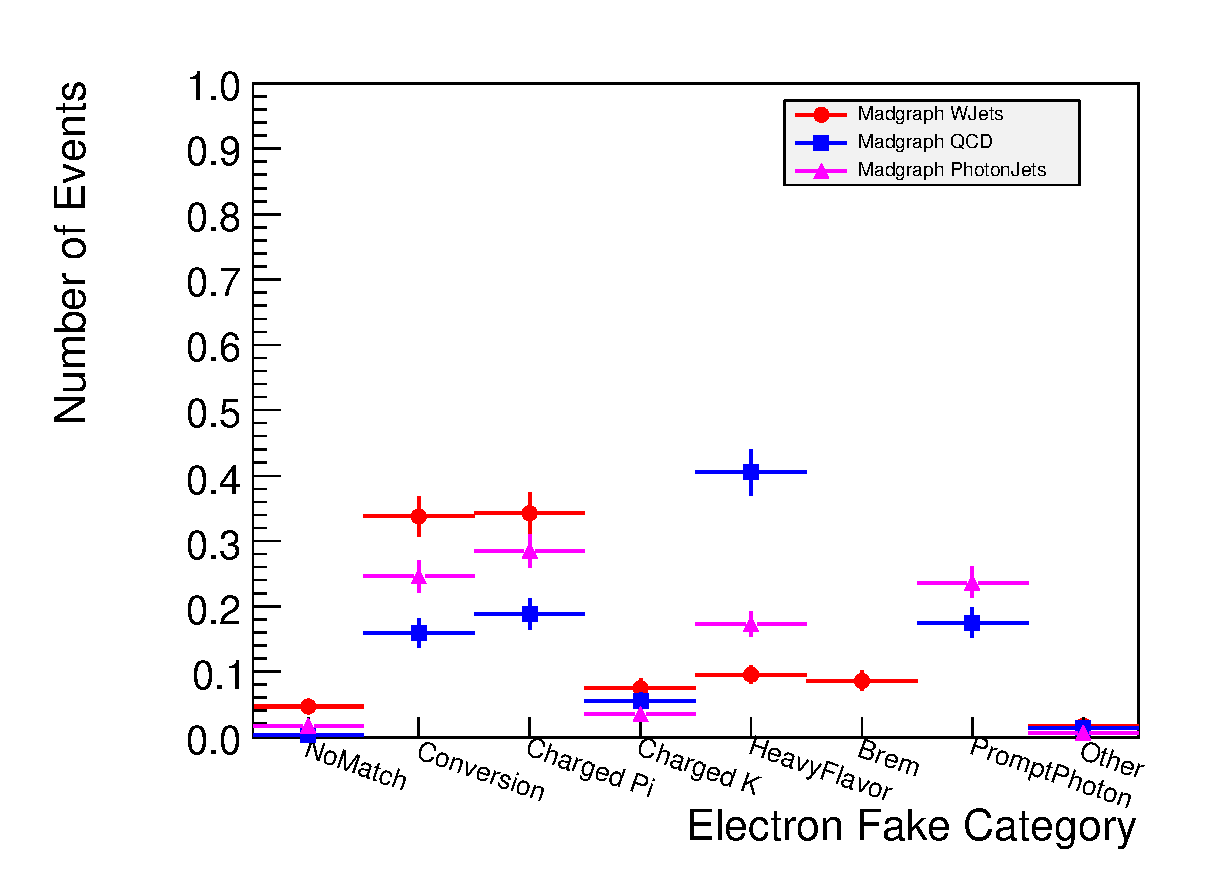
\includegraphics[width=0.49\textwidth]{plots/ElectronNumeratorFakeCategory_Madgraph_WJetsVsQCD.eps}
   \caption{Fraction of fake electron numerators in each category. The W+Jets sample is plotted in red, the QCD sample is plotted in blue, and the Photon+Jets sample is plotted in magenta.}
   \label{fig:ElectronNumerator_FakeCategory}
\end{center}
\end{figure}

\begin{figure}[htb]
\begin{center}
    \subfigure[]{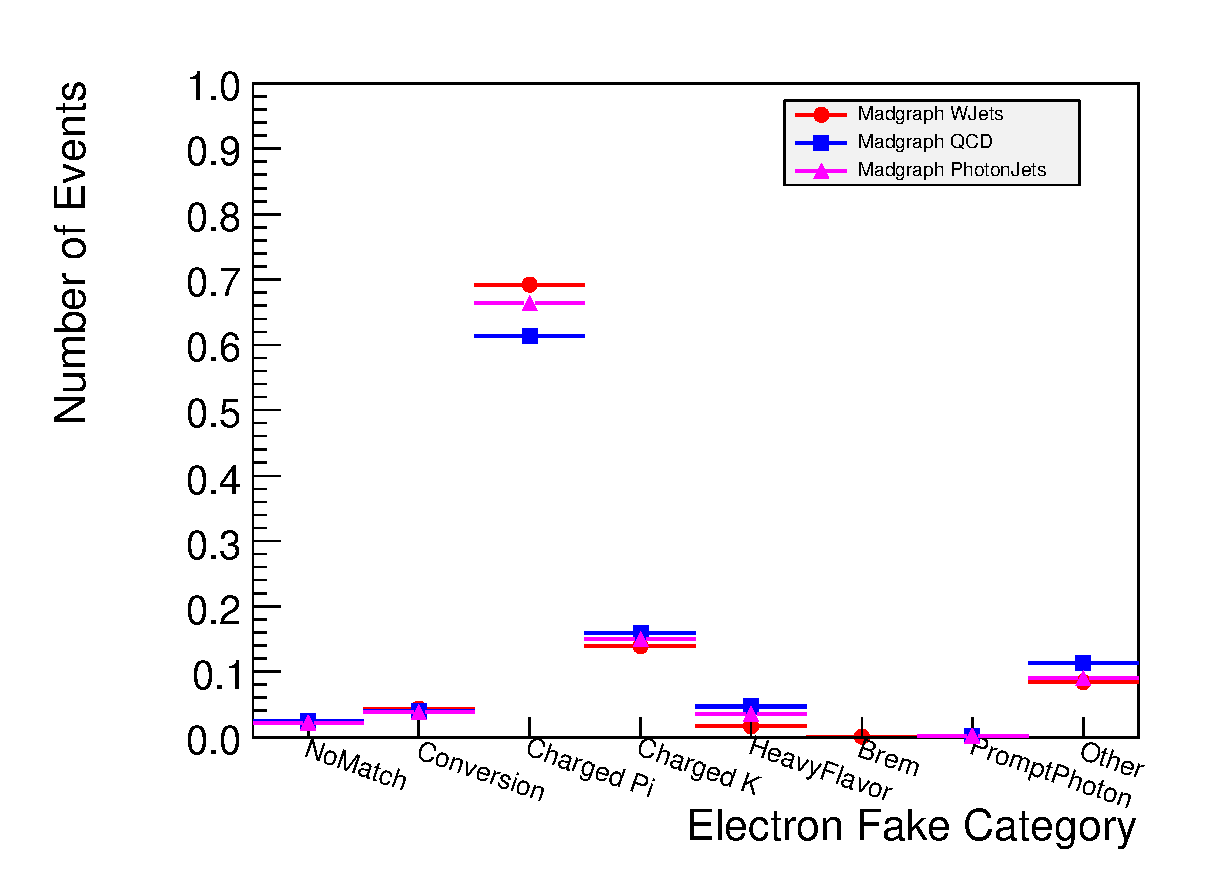
\includegraphics[width=0.49\textwidth]{plots/GsfTrackElectronDenominatorFakeCategory_Madgraph_WJetsVsQCD.eps}}
    \subfigure[]{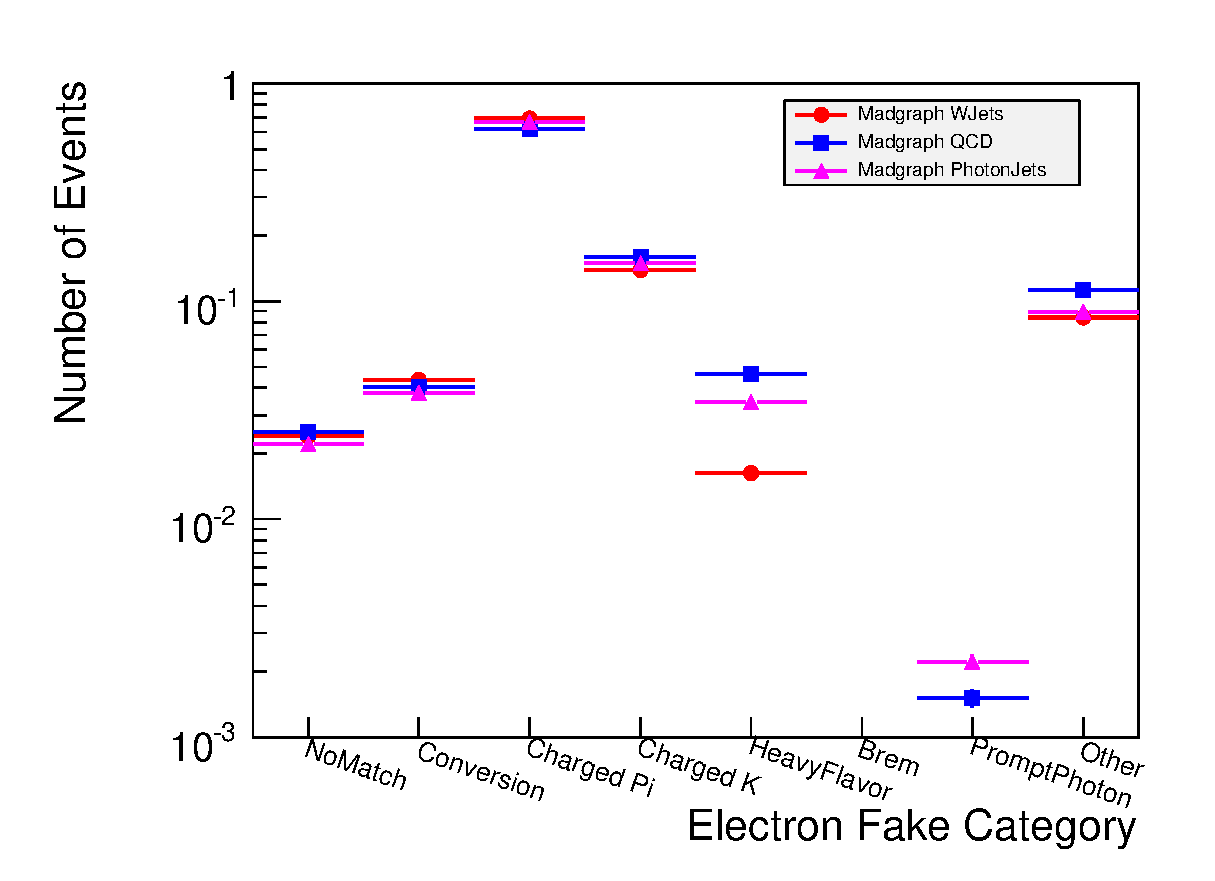
\includegraphics[width=0.49\textwidth]{plots/GsfTrackElectronDenominatorFakeCategory_Madgraph_WJetsVsQCD_logY.eps}}    
   \caption{The fraction of fake electron GsfTrack denominators in each category. The plot is shown in linear scale in (a) and log scale in (b). The color scheme is as in \FigureRef{fig:ElectronNumerator_FakeCategory}.}
   \label{fig:ElectronGsfTrackDenominatorFakeCategory}
\end{center}
\end{figure}

In Figures~\ref{fig:ElectronGsfTrackDenominatorFakeCategory} and~\ref{fig:ElectronRecoDenominatorFakeCategory}, we show the same plot for GsfTrack and Reco electron denominators, respectively. Here we see considerably different behaviour. The majority of denominators (about $70\%$) come from the charged pion category, while the conversion and heavy flavor categories are much reduced. In addition the ``Other'' category gives a marginally significant contribution, which are mainly due to a leading proton; these are almost entirely removed by the numerator cuts. Furthermore the difference between the \WPlusJets\ and QCD sample is also reduced, but general trends still remain: fraction of heavy flavor is larger in QCD and the fraction of charged pions is larger in \WPlusJets. These qualitative features are generally true for both GsfTrack and Reco denominators. 


\begin{figure}[htb]
\begin{center}
    \subfigure[]{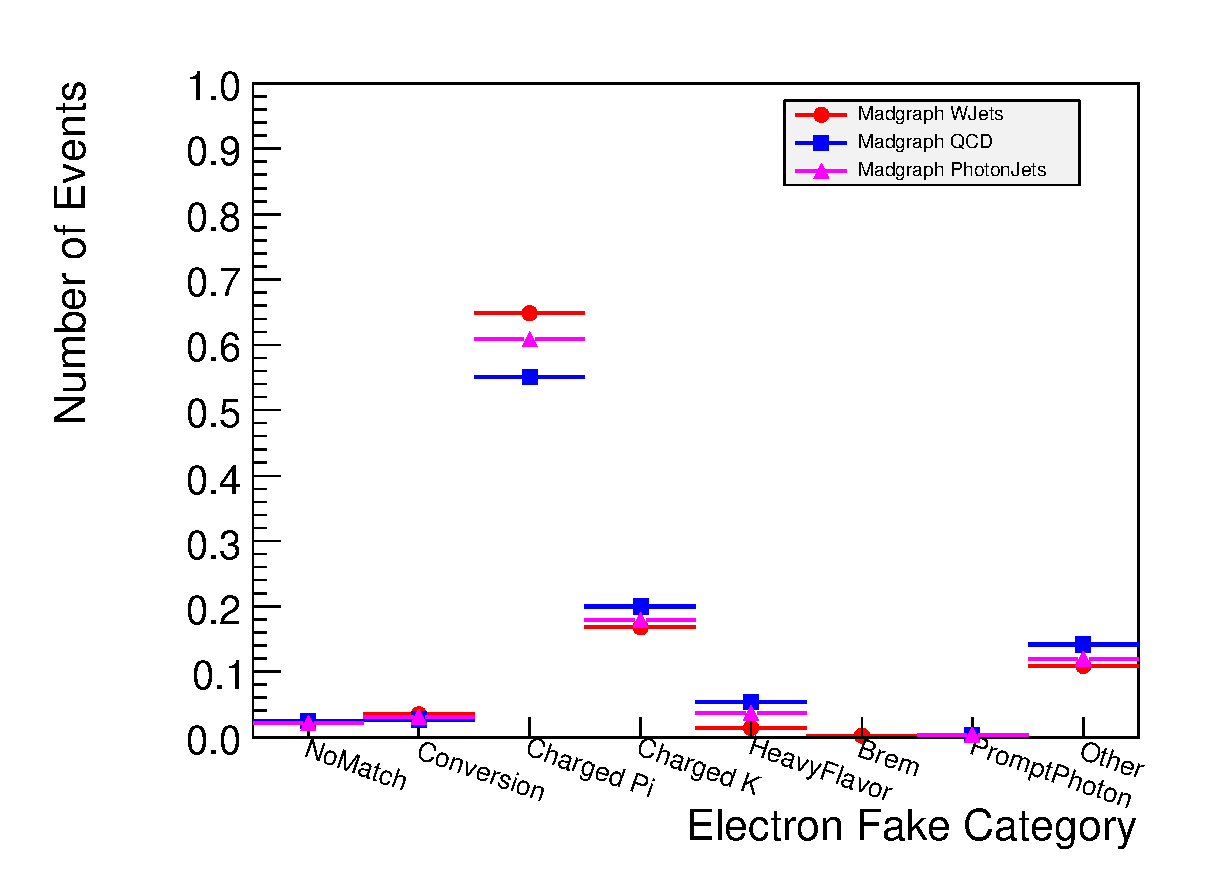
\includegraphics[width=0.49\textwidth]{plots/RecoElectronDenominatorFakeCategory_Madgraph_WJetsVsQCD.eps}}
    \subfigure[]{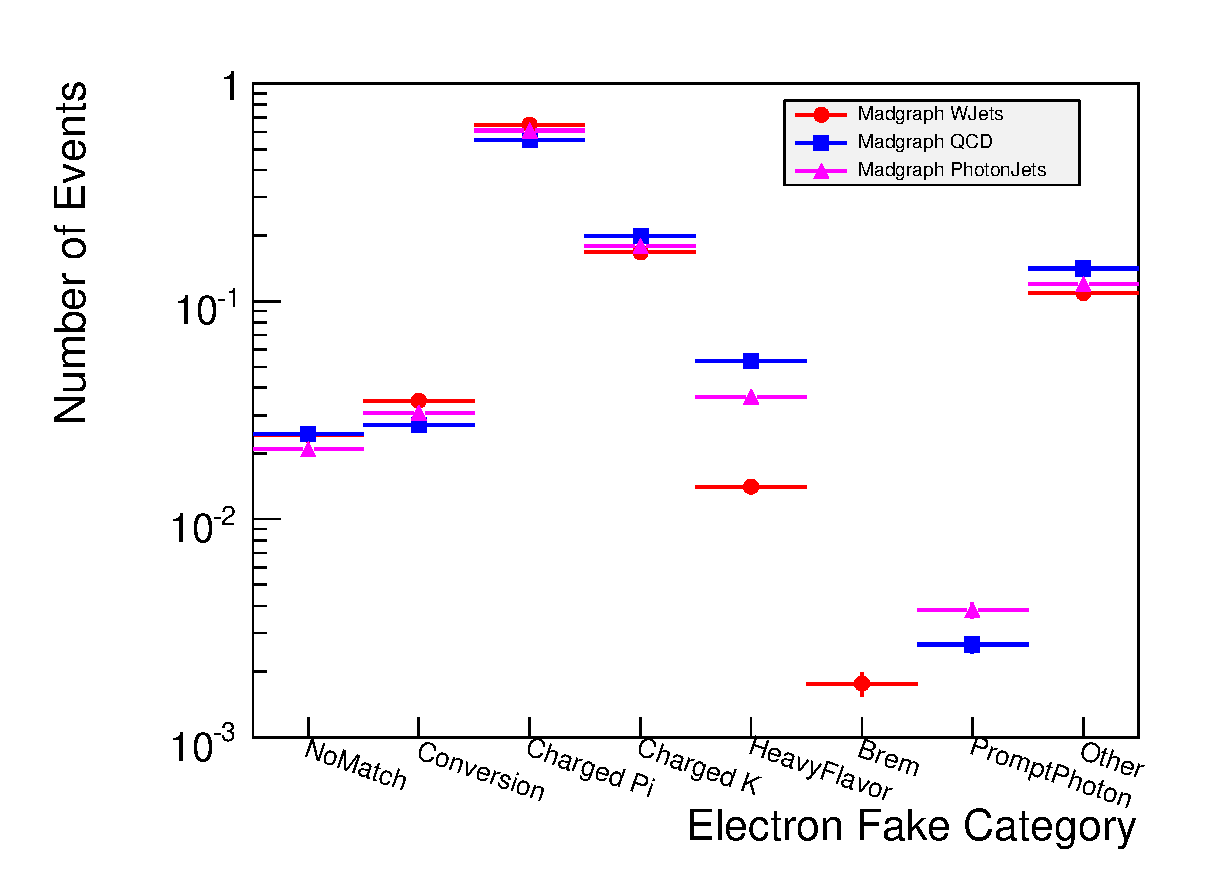
\includegraphics[width=0.49\textwidth]{plots/RecoElectronDenominatorFakeCategory_Madgraph_WJetsVsQCD_logY.eps}}    
   \caption{The fraction of fake electron Reco denominators in each category. The plot is shown in linear scale in (a) and log scale in (b). The color scheme is as in \FigureRef{fig:ElectronNumerator_FakeCategory}.}
   \label{fig:ElectronRecoDenominatorFakeCategory}
\end{center}
\end{figure}

In \FigureRef{fig:ElectronFakeRate_FakeCategory} we show the average fake rate for the two denominator definitions as a function of the electron fake category. The plot shows consistent fake rates between the \WPlusJets\ sample and the QCD sample when one separates into the various categories. For the Reco denominator, the fake rate for semi leptonic decay of heavy flavor hadrons and \pizero conversions are around $10\%$; the fake rate for charged pions and kaons are around $0.5\%$; the fake rate for isolated photons are roughly $50\%$.

\begin{figure}[htb]
\begin{center}
    \subfigure[]{\includegraphics[width=0.49\textwidth]{plots/GsfTrackElectronFakeRate_FakeCategory_Madgraph.eps}}
    \subfigure[]{\includegraphics[width=0.49\textwidth]{plots/RecoElectronFakeRate_FakeCategory_Madgraph.eps}}    
   \caption{The overall electron fake rate as a function of the electron fake category for GsfTrack denominators (a) and Reco denominators (b). The color scheme is as in \FigureRef{fig:ElectronNumerator_FakeCategory}.}
   \label{fig:ElectronFakeRate_FakeCategory}
\end{center}
\end{figure}

\customSubsubsection{Fake Electron Jet Flavor}
Another way to study the underlying fake mechanism is to study the flavor content of the jets which fake electrons. For a given fake numerator or denominator, we match to the nearest generator level jet, obtained by clustering generator level particles (GenJet), with $\Delta R < 0.5$ and then find its flavor. \FigureRef{fig:ElectronNumerator_JetFlavor} shows the jet flavor composition of the fake electron numerators in the \WPlusJets\ and QCD sample. We see that generally the QCD sample has a greater fraction of fakes from b quarks while the \WPlusJets\ sample has a greater fraction from light quarks. In the \WPlusJets\ sample there are are a significant fraction of events which have no GenJet nearby indicating that the fake was likely due to an isolated photon. In \FigureRef{fig:ElectronDenominator_JetFlavor} we show the same distribution for the denominators. The trend described for the numerator is seen for denominators as well. In addition we see that the contribution of gluons is much larger in the QCD sample than in the \WPlusJets\ sample. 

\begin{figure}[htb]
\begin{center}
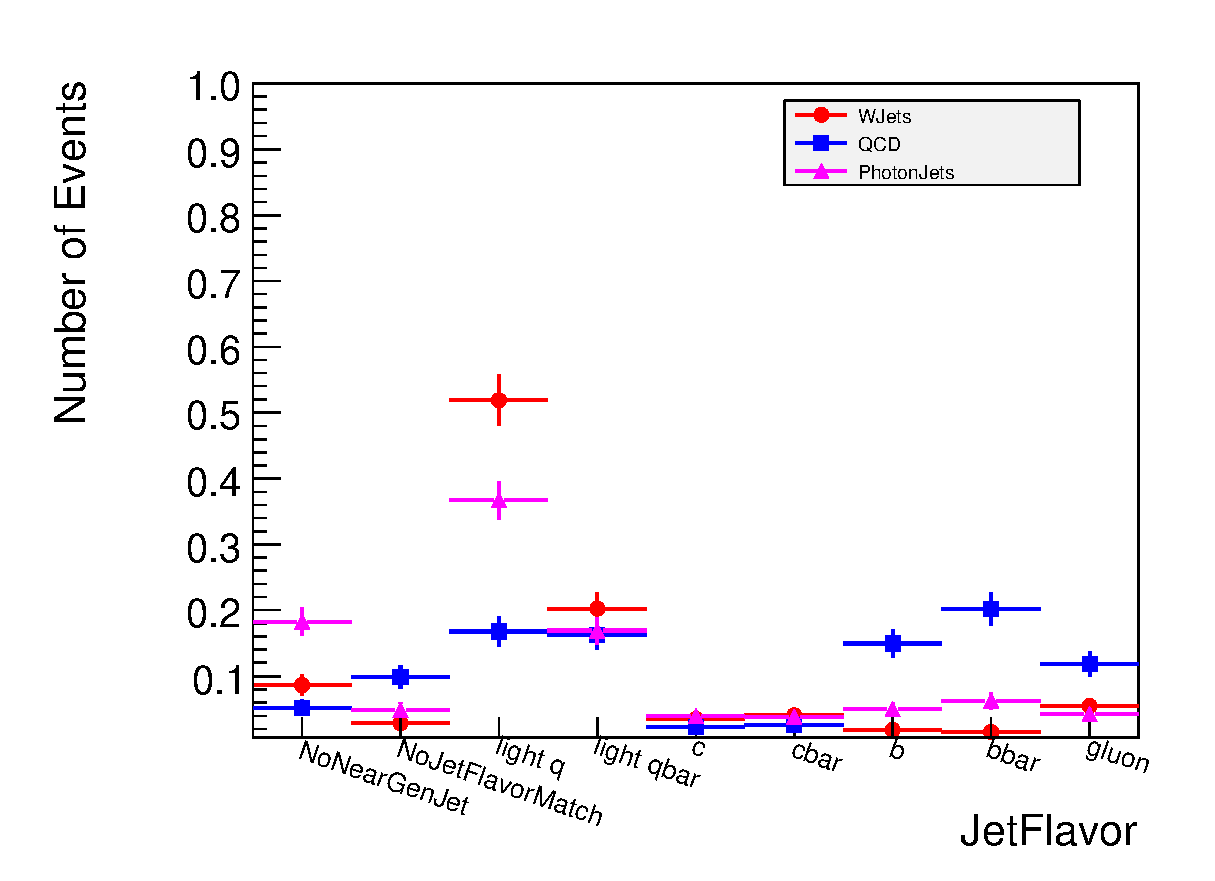
\includegraphics[width=0.49\textwidth]{plots/ElectronNumeratorJetFlavor_Madgraph_WJetsVsQCD.eps}
   \caption{Fraction of fake electron numerators matched to the shown GenJet flavor. The color scheme is as in \FigureRef{fig:ElectronNumerator_FakeCategory}. }
   \label{fig:ElectronNumerator_JetFlavor}
\end{center}
\end{figure}

In \FigureRef{fig:ElectronFakeRate_JetFlavor} we show the fake rate as a function of the matched GenJet flavor. The fake rates for gluons are roughly a factor of 2 smaller than the fake rates for quark jets. In addition the fake rate for b quarks are around 5 to 10 times larger than the fake rate for light quarks. Since gluons account for a larger fraction of the denominator in the QCD sample, one expects that the fake rate measured in a QCD enhanced sample is generally smaller than the fake rate measured in a sample of \WPlusJets\ events. The uncertainty in the difference of the gluon fraction in the two samples contribute yet another important unknown systematic effect.    

\begin{figure}[htb]
\begin{center}
    \subfigure[]{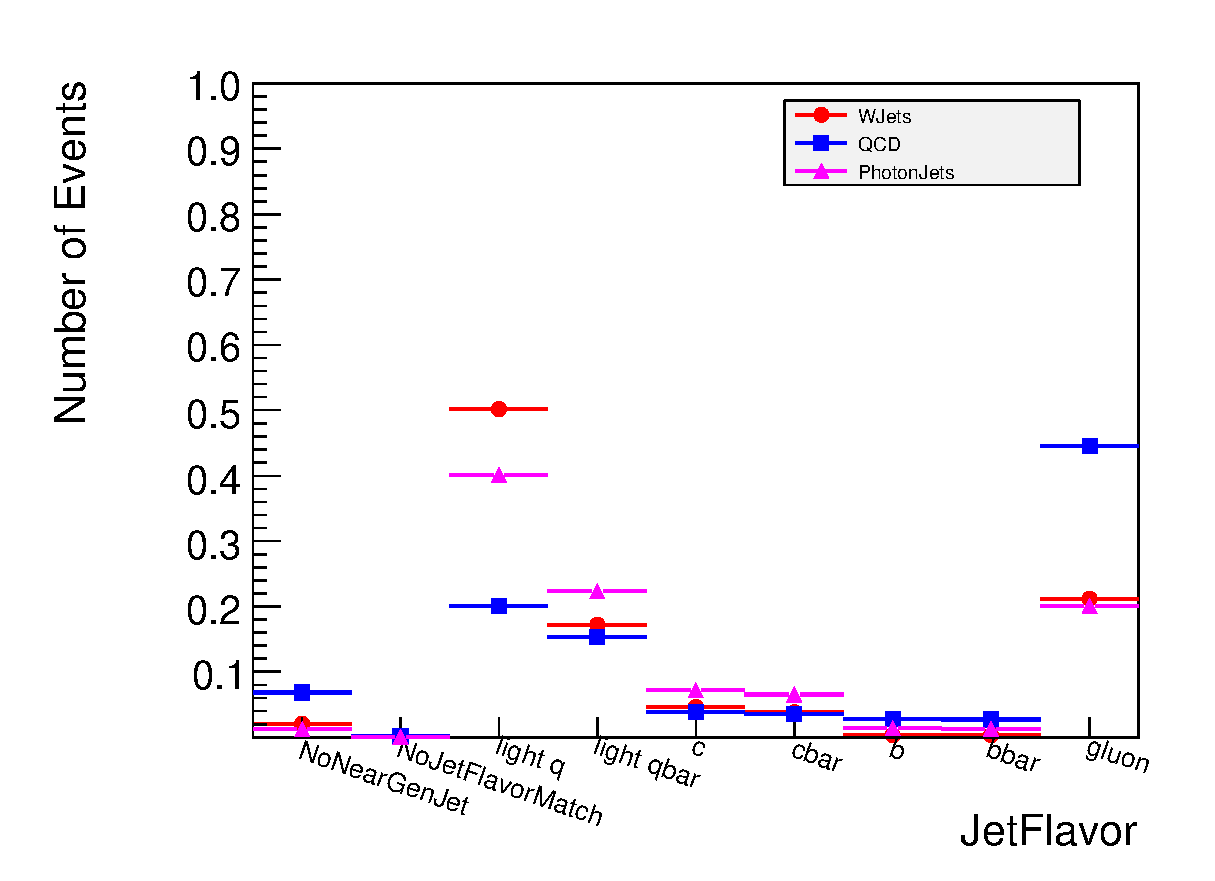
\includegraphics[width=0.49\textwidth]{plots/GsfTrackElectronDenominatorJetFlavor_Madgraph_WJetsVsQCD.eps}}    
    \subfigure[]{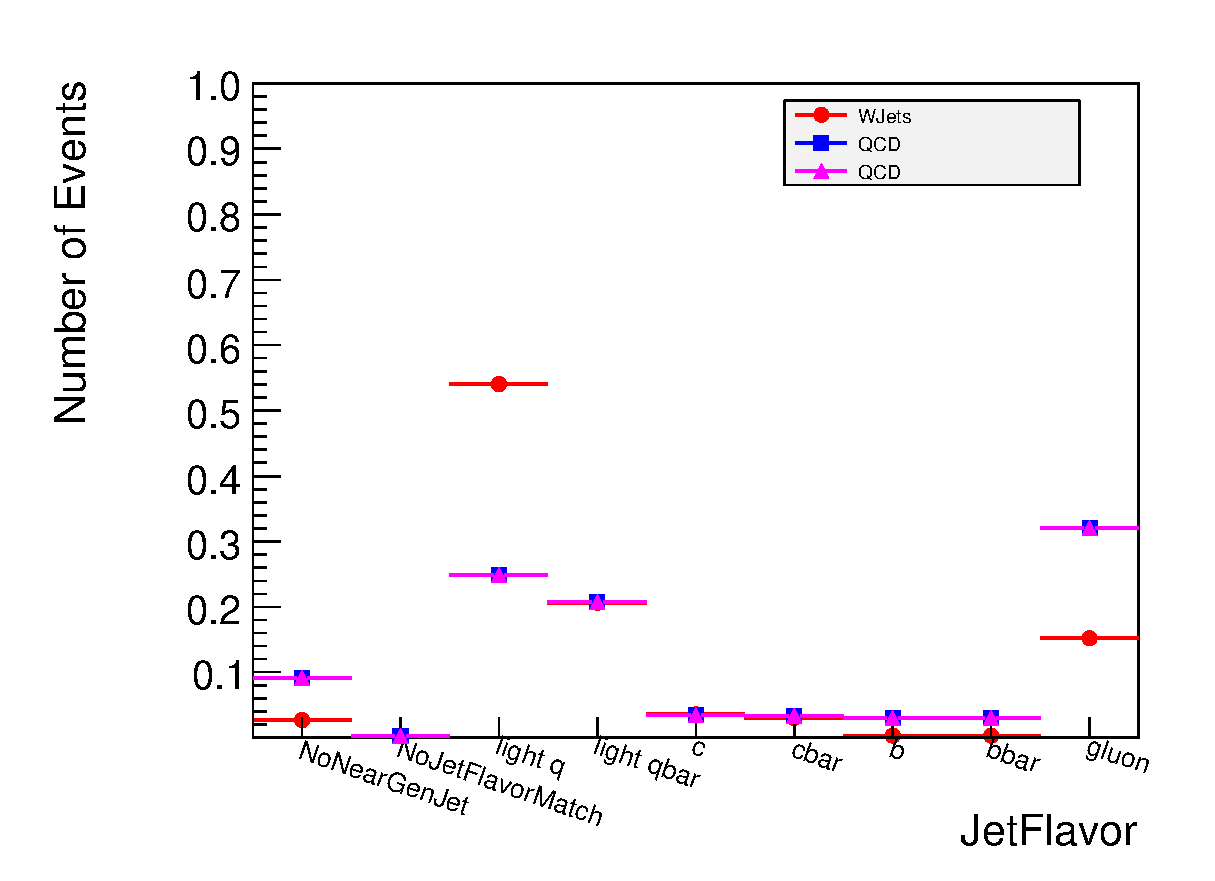
\includegraphics[width=0.49\textwidth]{plots/RecoElectronDenominatorJetFlavor_Madgraph_WJetsVsQCD.eps}}
   \caption{Fraction of fake electron GsfTrack denominators (a) and Reco denominators (b) matched to the shown GenJet flavor. The color scheme is as in \FigureRef{fig:ElectronNumerator_FakeCategory}.}
   \label{fig:ElectronDenominator_JetFlavor}
\end{center}
\end{figure}

\begin{figure}[htb]
\begin{center}
    \subfigure[]{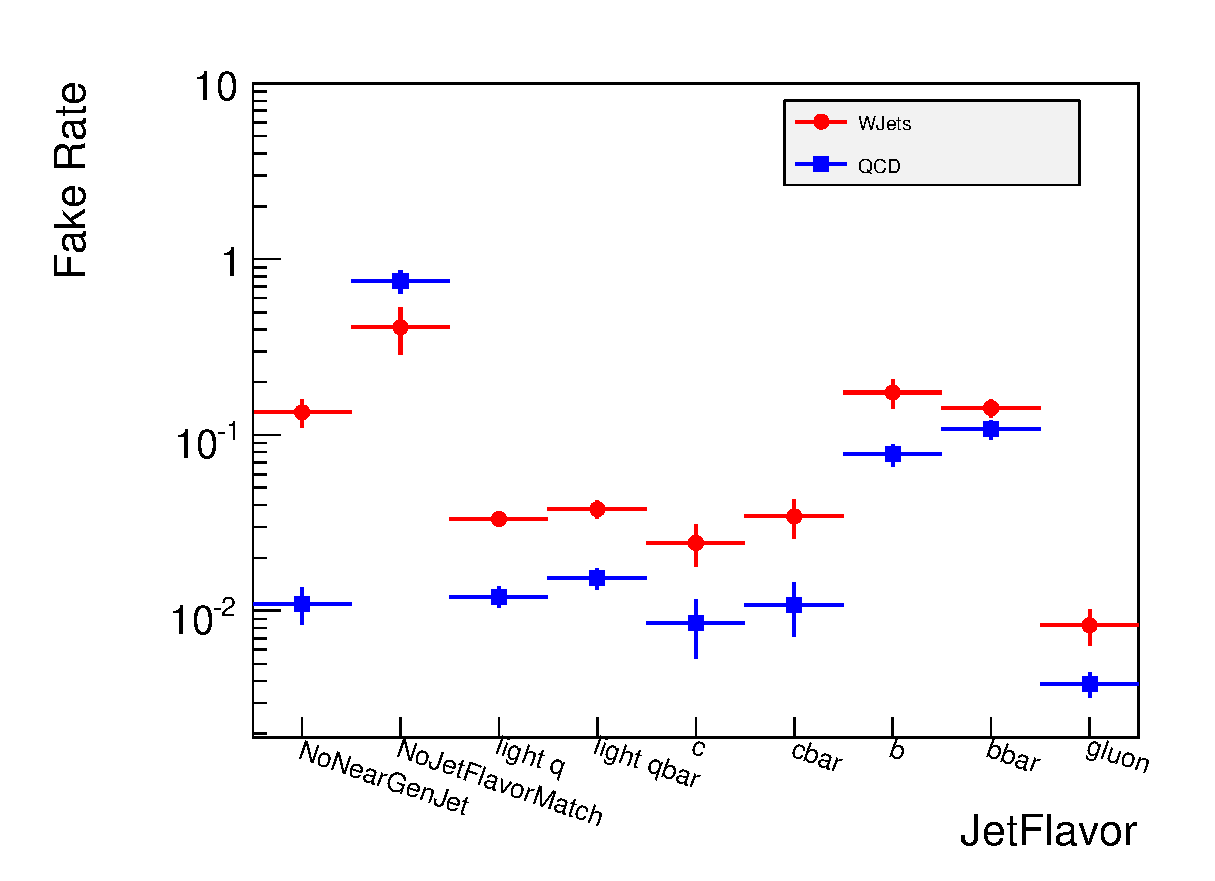
\includegraphics[width=0.49\textwidth]{plots/GsfTrackElectronFakeRateJetFlavor_Madgraph_WJetsVsQCD.eps}}    
    \subfigure[]{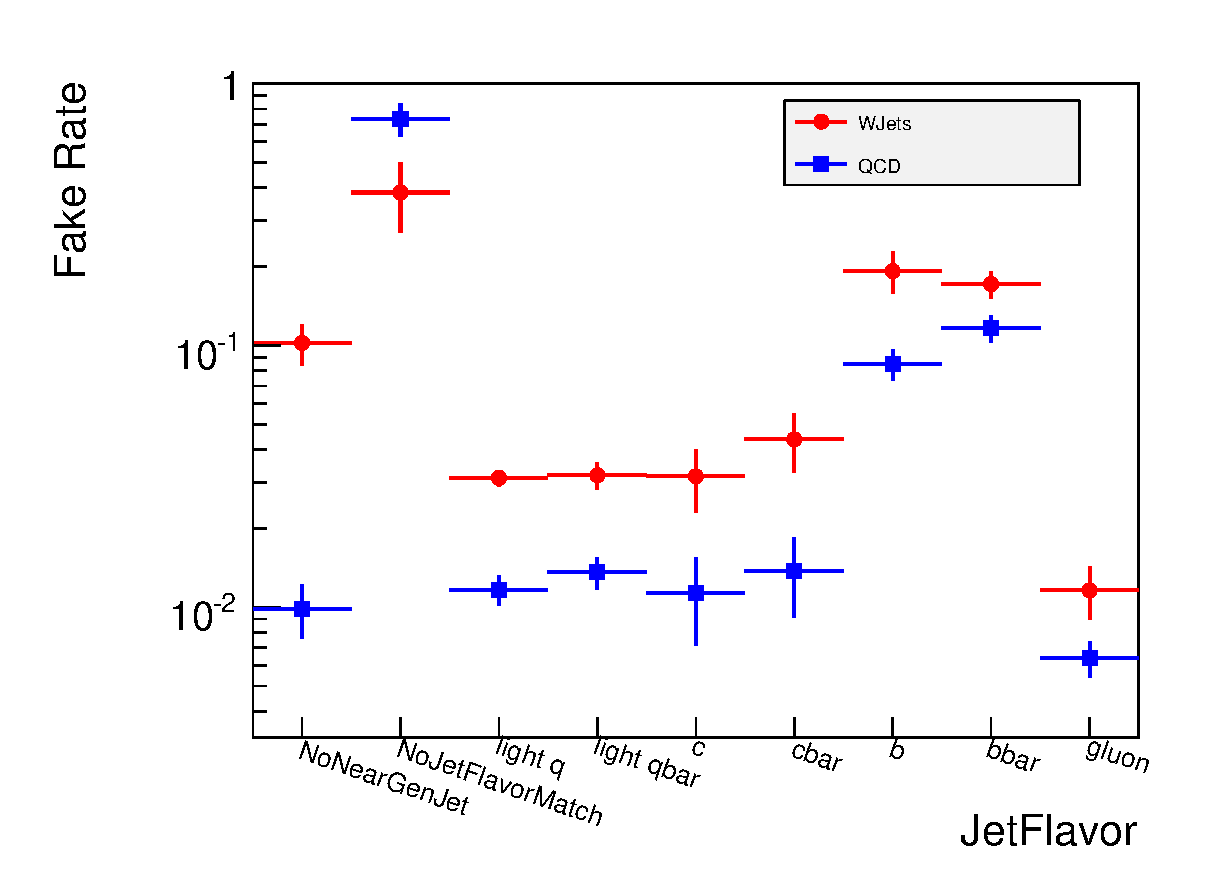
\includegraphics[width=0.49\textwidth]{plots/RecoElectronFakeRateJetFlavor_Madgraph_WJetsVsQCD.eps}}
   \caption{The overall electron fake rate as a function of the matched GenJet Flavor for GsfTrack denominators (a) and Reco denominators (b). The color scheme is as in \FigureRef{fig:ElectronNumerator_FakeCategory}.}
   \label{fig:ElectronFakeRate_JetFlavor}
\end{center}
\end{figure}


\customSubsubsection{Contamination of Isolated Photons}
One very important feature from Figures~\ref{fig:ElectronNumerator_FakeCategory},~\ref{fig:ElectronGsfTrackDenominatorFakeCategory}, and~\ref{fig:ElectronRecoDenominatorFakeCategory} are the fraction of numerators and denominators coming from hard bremstrahlung off of the lepton from \WPM\ decay in tracker material in the \WPlusJets\ sample, and those coming from an isolated prompt photon in the jet-triggered sample. In this Monte Carlo study we find that these two fractions are actually surprisingly similar. This is likely simply a coincidence since they come from entirely different processes altogether. Depending on how well the current simulation is modelling the real detector, we expect these numbers to be possibly different in data. The difference between these fractions will be an important unknown in the data sample. Unfortunately classification algorithms of this kind cannot be applied in data. However doing these types of studies in simulation will give us better understanding of this effect. 


\customSubsubsection{Charged Pion Fakes Versus \pizero\ Conversion Fakes}
\label{sec:systematics_chargecorrelation}
From \FigureRef{fig:ElectronFakeRate_FakeCategory}, we observe that the fake rate for charged pion fakes is much smaller than the fake rate for \pizero\ conversion fakes. Essentially this tells us that the probability for a charged pion to undergo charge exchange is much smaller than the probability for \pizero\ to decay asymmetrically followed by an asymmetric conversion. However due to the fact that the denominator samples have a much larger fraction of charged pion fakes, the relative importance for the numerator becomes similar. However, the fraction of charged pions and \pizero\ conversion fakes is not necessarily expected to be the same in the calibration and extrapolation sample. Figures~\ref{fig:ElectronGsfTrackDenominatorFakeCategory} and \ref{fig:ElectronRecoDenominatorFakeCategory} give an idea of the difference we expect to see in the relative importance of these two categories in the Monte Carlo simulation for the calibration sample (jet-triggered sample or photon-triggered sample) and the extrapolation sample (\WPlusJets\ sample). 

%Furthermore, there are differences in the fake rates for quark jets and gluon jets, even within these categories. The total fake rate for the \pizero\ conversion category as a function of the underlying jet flavor. The fake rates for quark jets are significantly larger than those for gluon jets. A similar effect is seen in FigNN where we have made the same plot but for the charged pion category. This difference is essentially due to the fact the probability for a quark to fragment to a leading pion carrying almost all the energy of the quark is greater than this probability for a gluon. 

In the two lepton final state, this difference is expected to have a significant effect on the charge correlation between the real lepton from a \WPM\ decay and the fake lepton. This charge correlation is essentially from the charge correlation between the \WPM\ and a quark in events where a \WPM\ was produced in association with a quark. In order for a jet to be able to fake an isolated electron, it almost always has to fragment into a leading hadron carrying almost all the energy of the original parton. In this case, the charge of the original quark is largely preserved in the charge of this leading hadron. In the case of the charged pion and charged kaon fakes, the track that is reconstructed as an electron track carries the charge of the leading pion or kaon and the charge correlation with the \WPM\ is preserved. In the case of a leading \pizero, the \pizero will decay to two photons which then undergoes conversion in the tracker material. Since the conversion is random with respect to the charge of the leading leg, the charge correlation is essentially removed for this category of fakes. This is further affected by the contamination of isolated photons in the extrapolation sample. As a result, the correctness of the charge correlation between the two leptons in our prediction depends critically on the fraction of fakes coming from conversions versus the fraction of fakes coming from the other processes. Since the calibration sample contains a minimal amount of fakes due to isolated photons, we do not expect this feature to be modelled particularly well with this method. 

This effect is particularly enhanced for the \WPlusGamma\ process since the photon to electron fake rate is much larger than the rate for jets to fake electrons.  Since we clearly cannot reliably predict the charge correlation for \WPlusGamma\ events using the jet-triggered sample or the photon-triggered sample, 
we choose to remove this background from this method.

\customSubsection{Fake Muon Studies}
\customSubsubsection{Fake Muon Categories}
First, we study the composition of muon fakes in simulation. \FigureRef{fig:MuonNumerator_FakeCategory} shows the fraction of fake muon numerators in each of the categories. There is a large difference between the fake process composition in the \WPlusJets\ sample and the jet triggered or photon triggered sample. For the jet triggered and photon triggered sample, almost all numerators are due to semi-leptonic decays of \B\ or \D\ hadrons. For the \WPlusJets\ sample, however, it is much more evenly divided with heavy flavor accounting for about $50\%$, decays in flight accounting for about $30\%$, and punchthrough accounting for the remaining $20\%$. 

\begin{figure}[htb]
\begin{center}
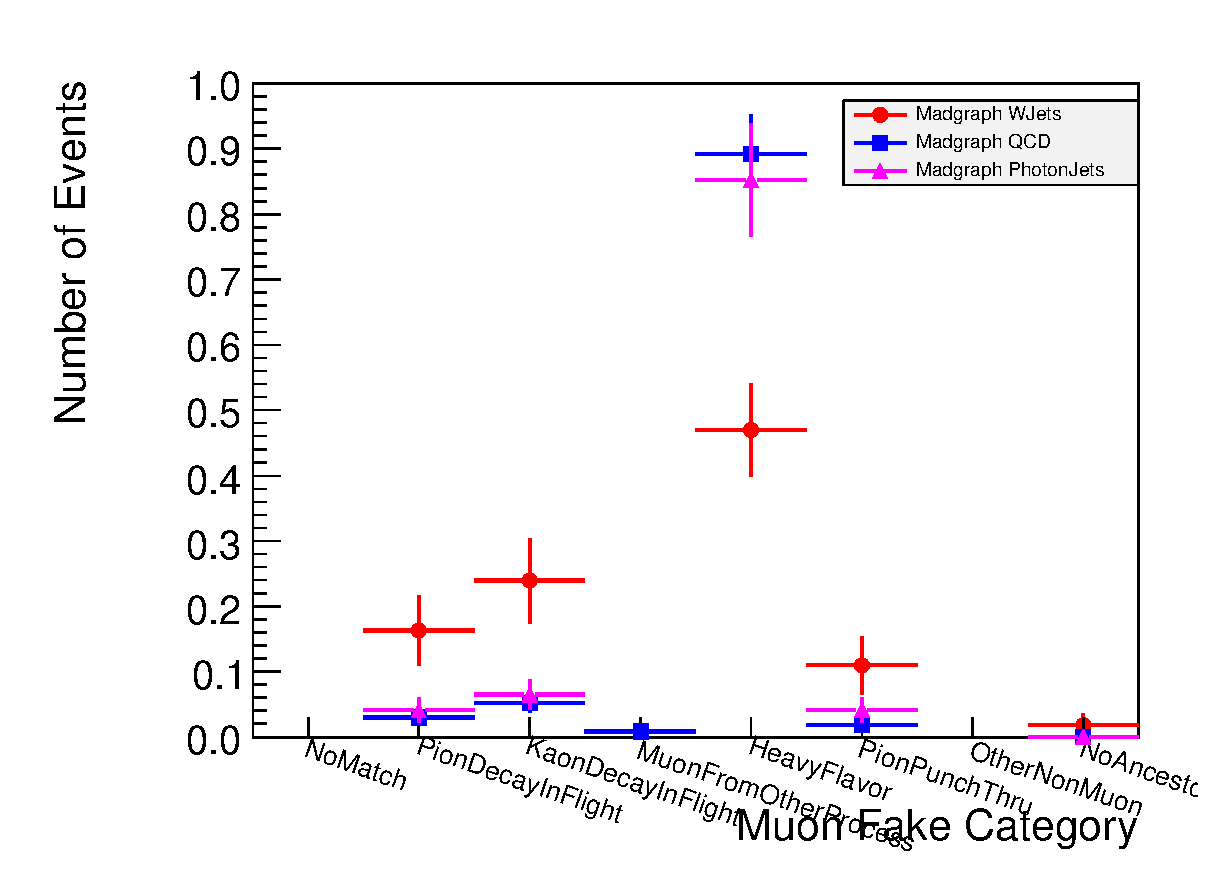
\includegraphics[width=0.49\textwidth]{plots/MuonNumeratorFakeCategory_Madgraph_WJetsVsQCD.eps}
   \caption{Fraction of fake muon numerators in each category. The color scheme is as in \FigureRef{fig:ElectronNumerator_FakeCategory}.}
   \label{fig:MuonNumerator_FakeCategory}
\end{center}
\end{figure}


In Figures~\ref{fig:MuonIsoTrackDenominatorFakeCategory},~\ref{fig:TrackerMuonDenominatorFakeCategory}, and~\ref{fig:GlobalMuonDenominatorFakeCategory} we show the fake composition for the isolated track, tracker muon, and global muon denominators respectively. For the isolated track denominator, the dominant contribution are expectedly from charged pion tracks, since the only requirement is a loosely isolated track. For both the tracker muon and global muon denominators, the main contributions are from heavy flavor semileptonic decays and punchthrough. However there are significant differences in the relative importance of these two categories among the \WPlusJets, and the jet triggered and photon triggered samples. In the jet triggered and photon triggered samples, the semileptonic decays are dominant, accounting for 60\% of the tracker muon denominators and 80\% of the global muon denominators. For the \WPlusJets\ sample, the punchthrough process is relatively more important and accounts for nearly 50\% of the tracker muon denominators and 25\% of the global muon denominators. This difference is due to a greater occurrence of jets from a bottom quark in QCD events compared with the \WPlusJets\ events. 

\begin{figure}[htb]
\begin{center}
    \subfigure[]{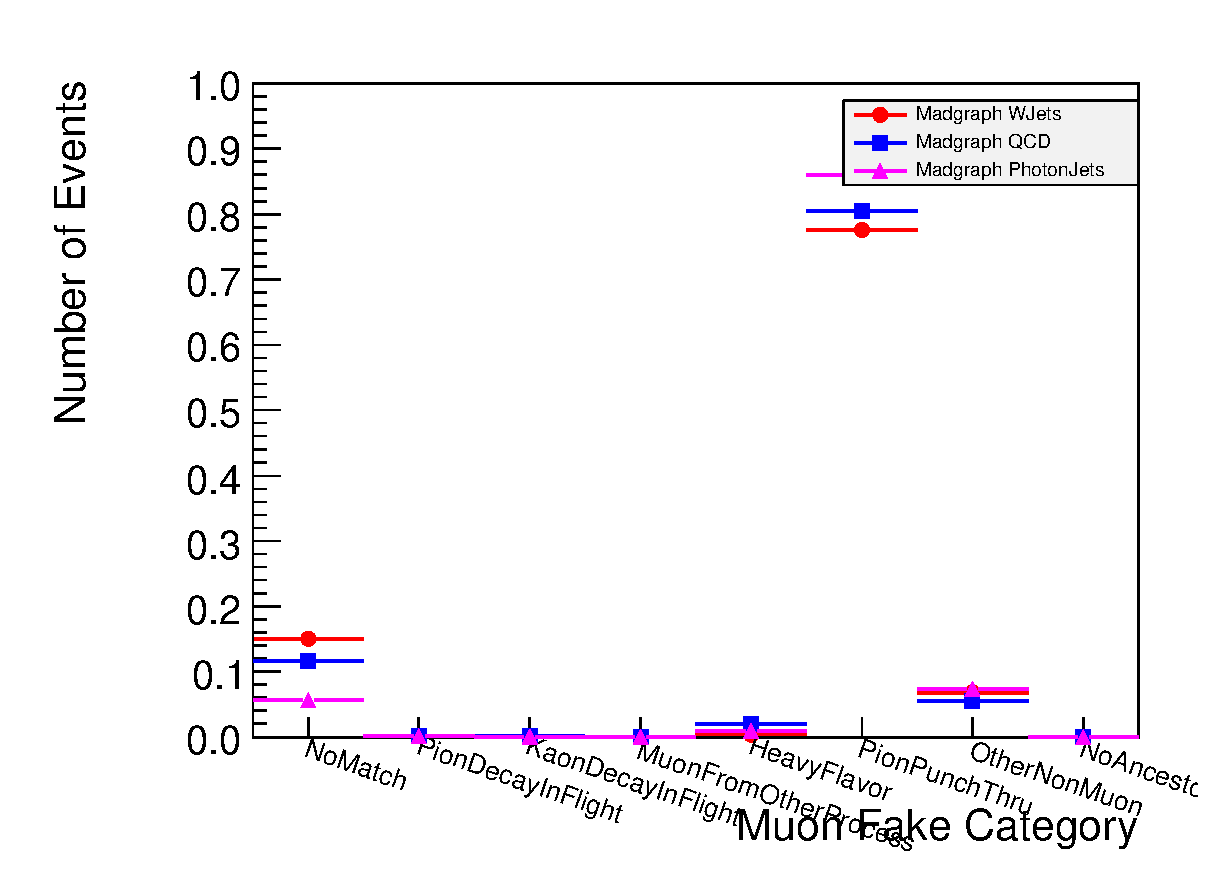
\includegraphics[width=0.49\textwidth]{plots/IsoTrackMuonDenominatorFakeCategory_Madgraph_WJetsVsQCD.eps}}
    \subfigure[]{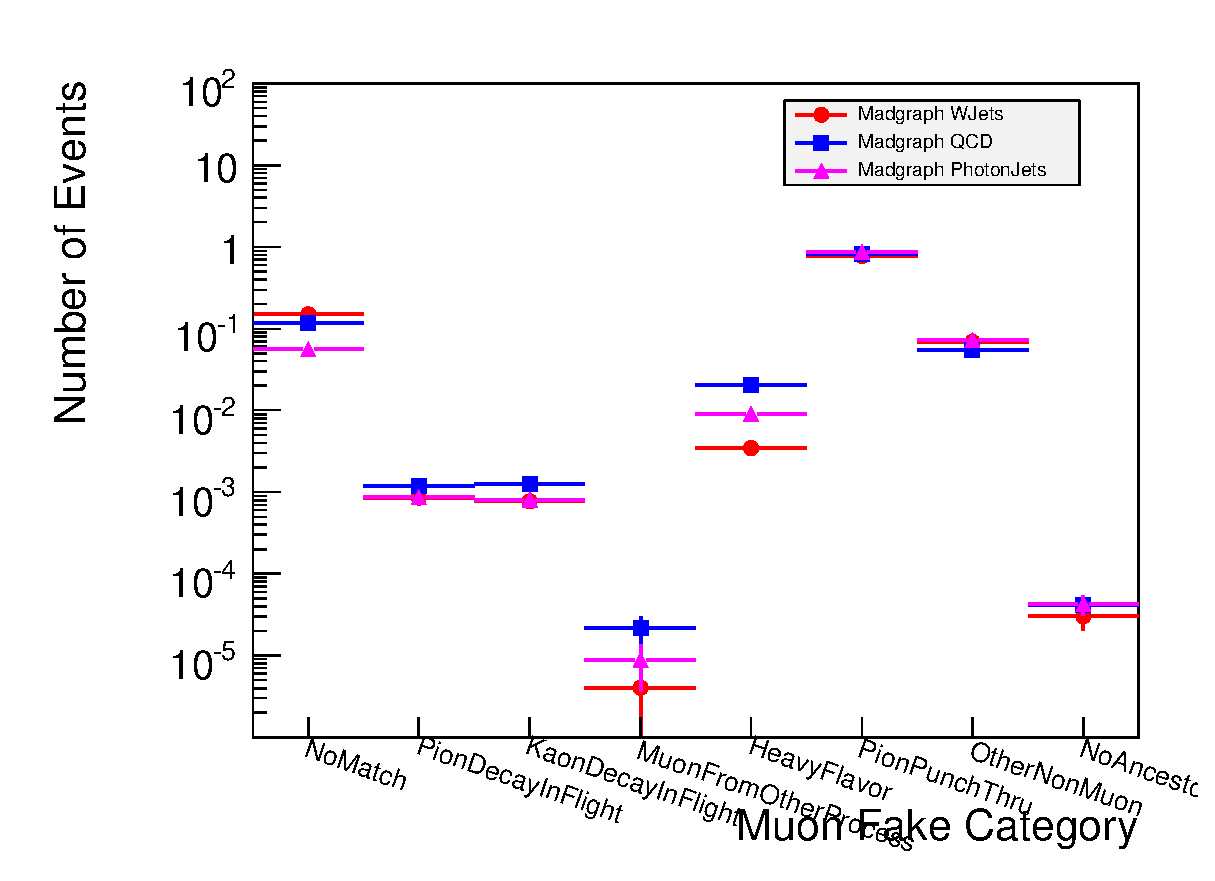
\includegraphics[width=0.49\textwidth]{plots/IsoTrackMuonDenominatorFakeCategory_Madgraph_WJetsVsQCD_logY.eps}}    
   \caption{The fraction of isolated track denominators in each category. The plot is shown in linear scale in (a) and log scale in (b). The color scheme is as in \FigureRef{fig:ElectronNumerator_FakeCategory}.}
   \label{fig:MuonIsoTrackDenominatorFakeCategory}
\end{center}
\end{figure}

\begin{figure}[htb]
\begin{center}
    \subfigure[]{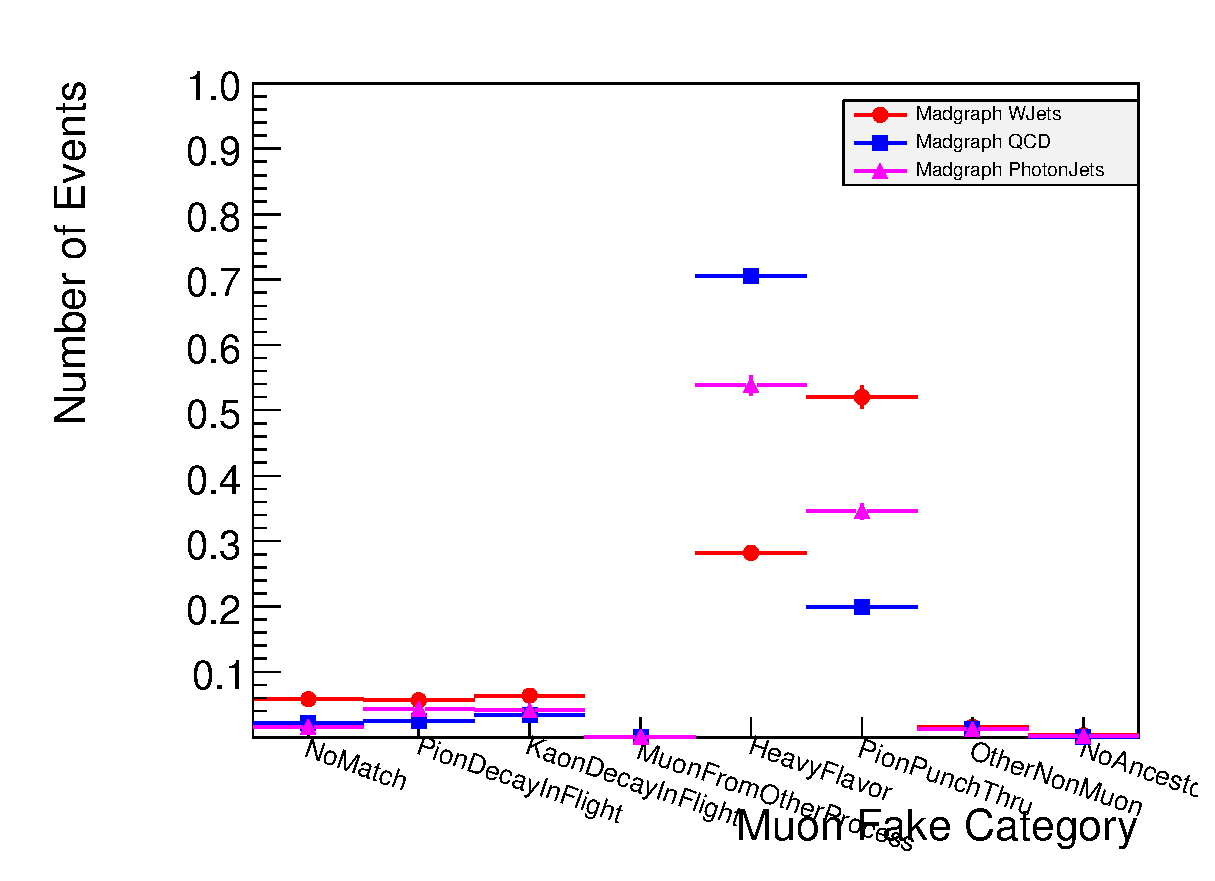
\includegraphics[width=0.49\textwidth]{plots/TrackerMuonDenominatorFakeCategory_Madgraph_WJetsVsQCD.eps}}
    \subfigure[]{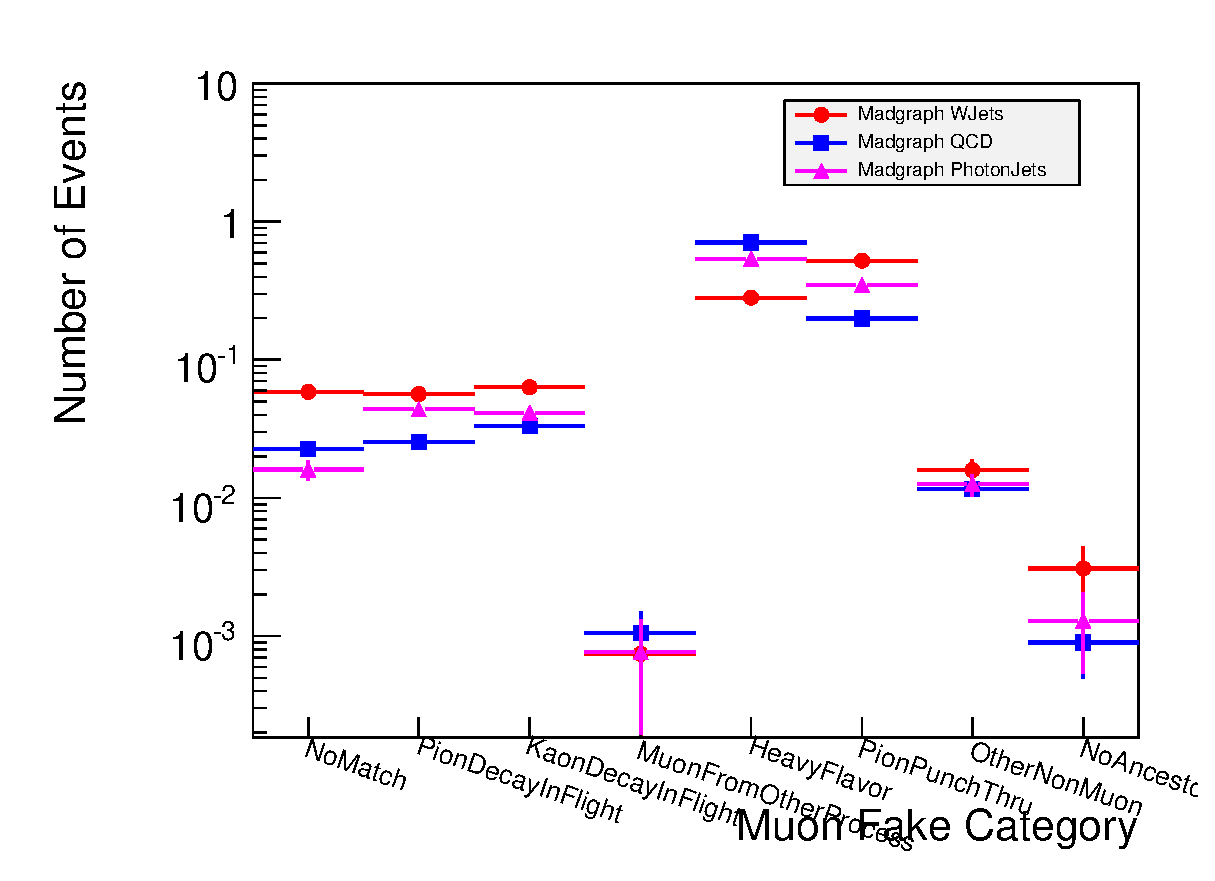
\includegraphics[width=0.49\textwidth]{plots/TrackerMuonDenominatorFakeCategory_Madgraph_WJetsVsQCD_logY.eps}}    
   \caption{The fraction of tracker muon denominators in each category. The plot is shown in linear scale in (a) and log scale in (b). The color scheme is as in \FigureRef{fig:ElectronNumerator_FakeCategory}.}
   \label{fig:TrackerMuonDenominatorFakeCategory}
\end{center}
\end{figure}

\begin{figure}[htb]
\begin{center}
    \subfigure[]{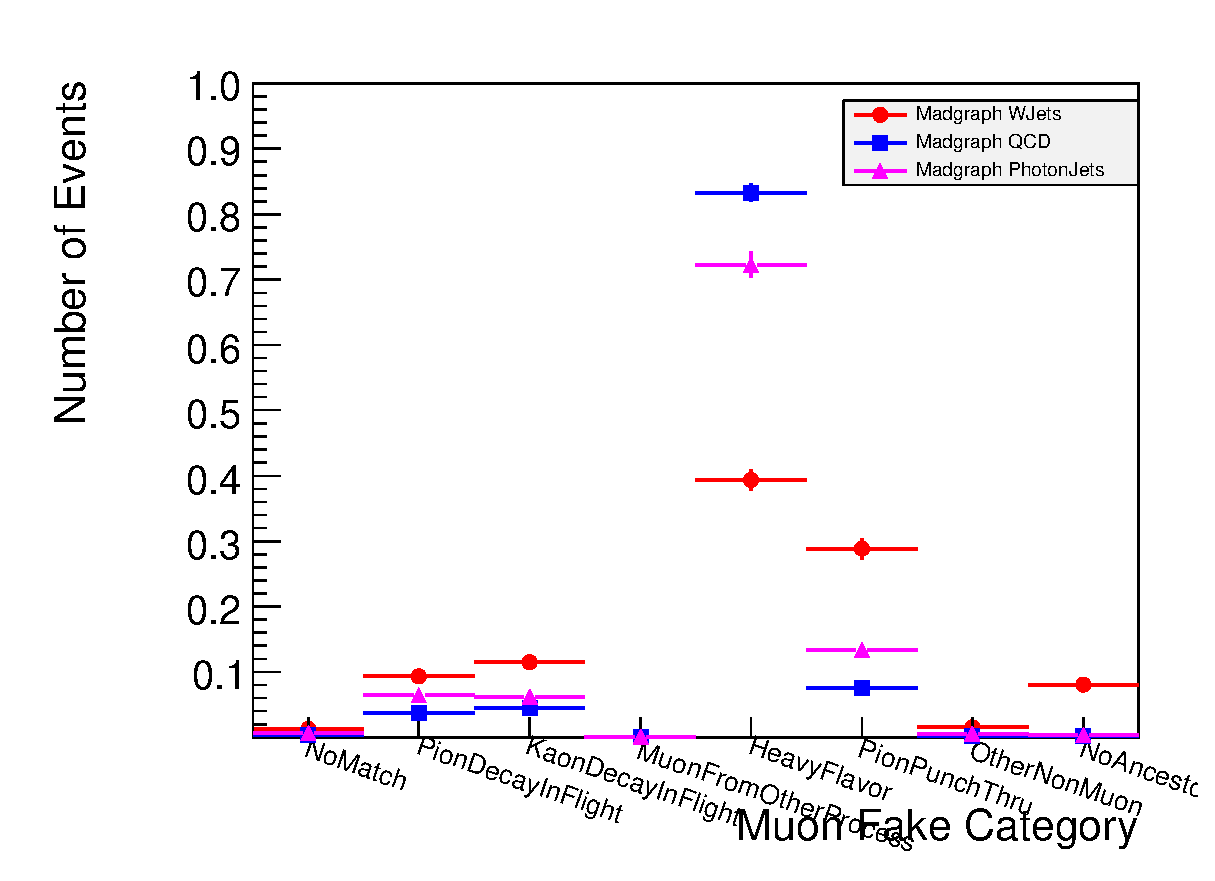
\includegraphics[width=0.49\textwidth]{plots/GlobalMuonDenominatorFakeCategory_Madgraph_WJetsVsQCD.eps}}
    \subfigure[]{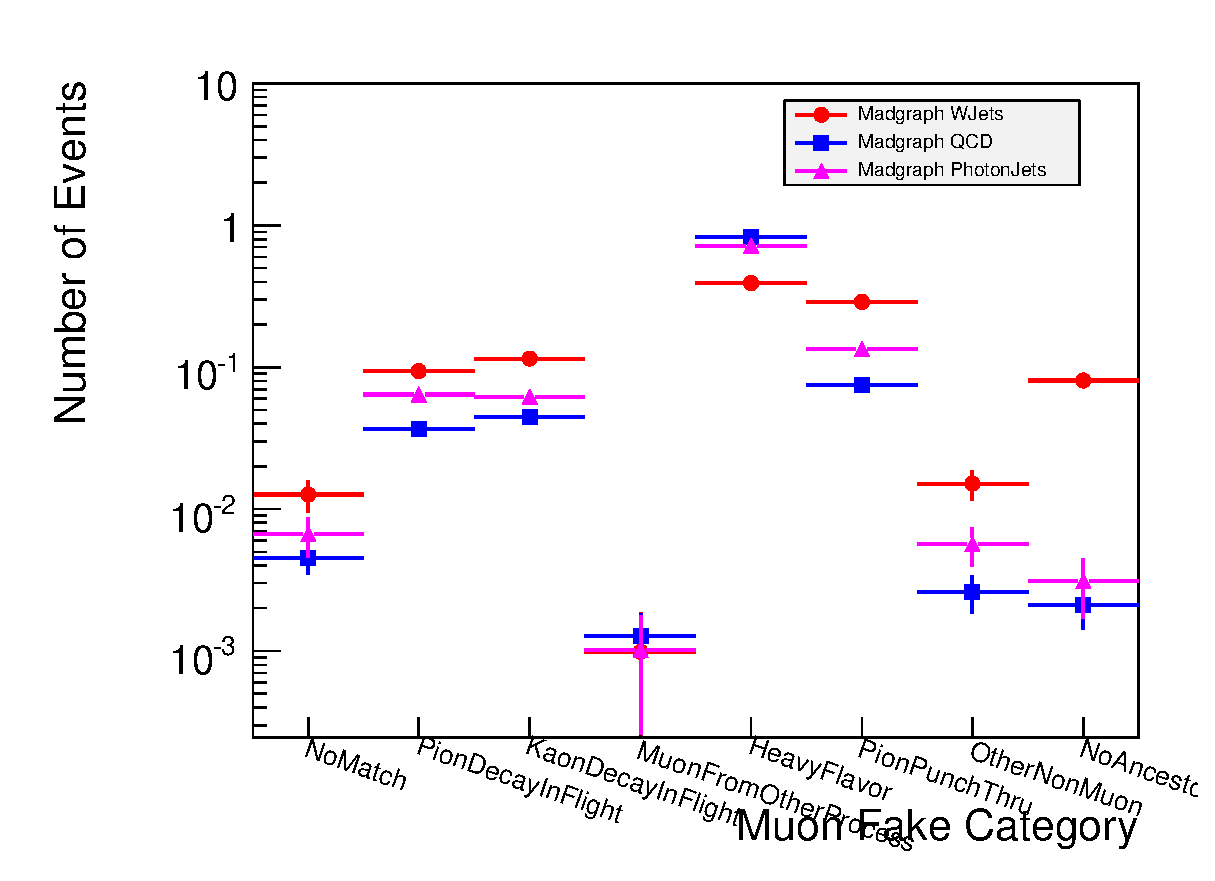
\includegraphics[width=0.49\textwidth]{plots/GlobalMuonDenominatorFakeCategory_Madgraph_WJetsVsQCD_logY.eps}}    
   \caption{The fraction of global muon denominators in each category. The plot is shown in linear scale in (a) and log scale in (b). The color scheme is as in \FigureRef{fig:ElectronNumerator_FakeCategory}.}
   \label{fig:GlobalMuonDenominatorFakeCategory}
\end{center}
\end{figure}

\clearpage

In Figures~\ref{fig:IsoTrackMuonFakeRate_FakeCategory},~\ref{fig:TrackerMuonFakeRate_FakeCategory}, and~\ref{fig:GlobalMuonFakeRate_FakeCategory}, we show the total fake rate as a function of the fake process. The behaviour is almost identical for the tracker muon and global muon denominators; the fake rates for semileptonic decays and decays in flight of pions and kaons are roughly $10\%$, while for punchthrough it is $1\%$ for the global muon denominator and $0.3\%$ for the tracker muon denominator. Fake rates for the isolated track denominator are significantly lower; for semileptonic decays and decays in flight, it is around a few percent, while for punchthrough it is on the order of $10^{-5}$.

\begin{figure}[htb]
\begin{center}    
    \subfigure[]{\includegraphics[width=0.49\textwidth]{plots/IsoTrackMuonFakeRate_FakeCategory_logY_Madgraph.eps}}    
   \caption{The overall muon fake rate using the isolated track denominator definition as a function of the fake category shown in log scale. The color scheme is as in \FigureRef{fig:ElectronNumerator_FakeCategory}.}
   \label{fig:IsoTrackMuonFakeRate_FakeCategory}
\end{center}
\end{figure}

\begin{figure}[htb]
\begin{center}
    \subfigure[]{\includegraphics[width=0.49\textwidth]{plots/TrackerMuonFakeRate_FakeCategory_logY_Madgraph.eps}}    
   \caption{The overall muon fake rate using the tracker muon denominator definition as a function of the fake category shown in linear scale (a) and log scale (b). The color scheme is as in \FigureRef{fig:ElectronNumerator_FakeCategory}.}
   \label{fig:TrackerMuonFakeRate_FakeCategory}
\end{center}
\end{figure}

\begin{figure}[htb]
\begin{center}
    \subfigure[]{\includegraphics[width=0.49\textwidth]{plots/GlobalMuonFakeRate_FakeCategory_logY_Madgraph.eps}}    
   \caption{The overall muon fake rate using the global muon denominator definition as a function of the fake category shown in linear scale (a) and log scale (b). The color scheme is as in \FigureRef{fig:ElectronNumerator_FakeCategory}.}
   \label{fig:GlobalMuonFakeRate_FakeCategory}
\end{center}
\end{figure}

The fact that the fake rates for semileptonic decays and decays in flight are roughly equal is encouraging, since it means that differences in the sample composition with respect to these two categories are not particularly important for the fake rate measurement. Control of the systematic uncertainties on muon fakes is essentially reduced to understanding the fraction of punchthrough in the different samples. This ensures that an understanding of muon fakes is made significantly easier compared to electrons, where multiple processes contribute significantly.


\customSubsubsection{Fake Muon Jet Flavor}
Finally, we study the jet flavor composition of fake muons. The fraction of fake muons matched to particular jet flavors is shown in \FigureRef{fig:MuonNumerator_JetFlavor}. For the jet triggered and photon triggered samples, the heavy flavor jets (bottom and charm) dominate the composition accounting for nearly $90\%$ of fake muons. For the \WPlusJets\ sample, there is a significant contribution due to light quarks accounting for roughly one quarter of fake muons in that sample. 

\begin{figure}[htb]
\begin{center}
  \subfigure[]{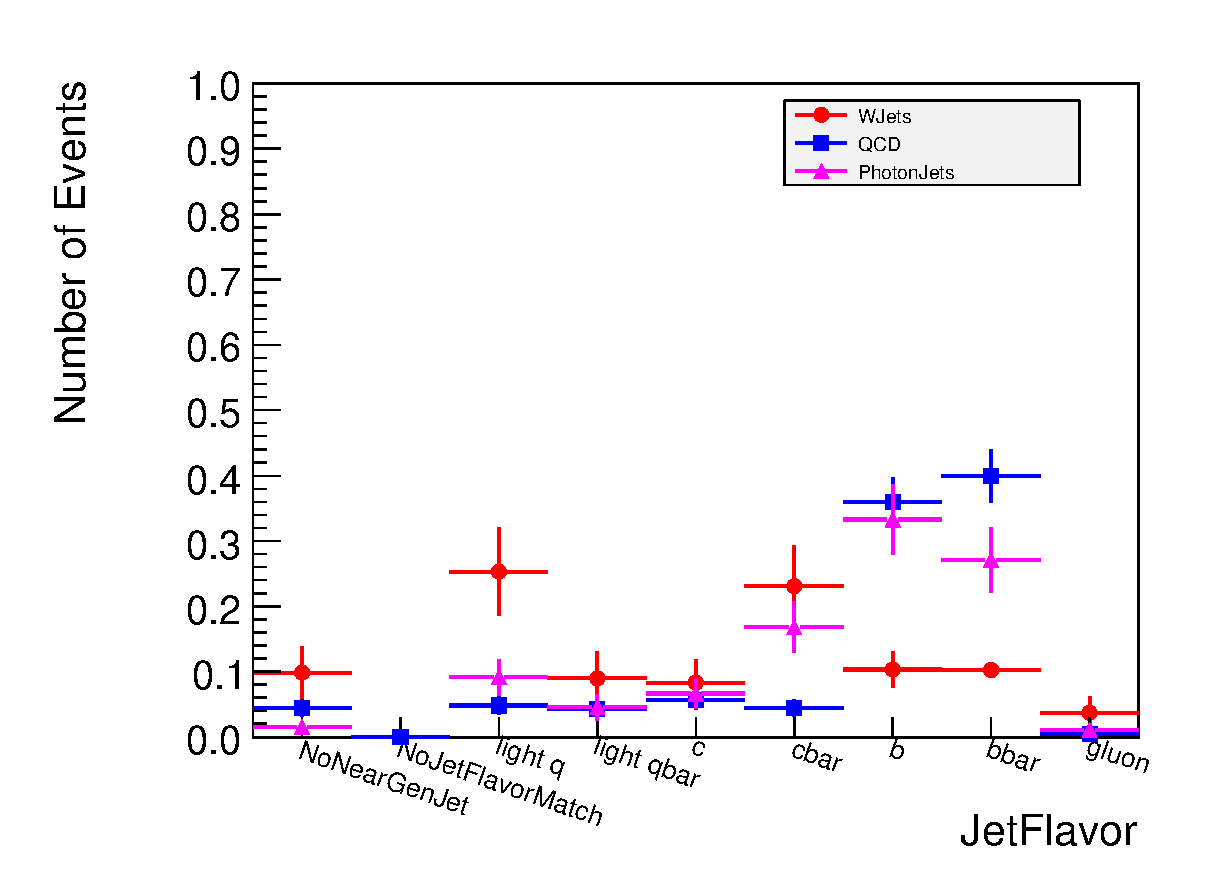
\includegraphics[width=0.49\textwidth]{plots/MuonNumeratorJetFlavor_Madgraph_WJetsVsQCD.eps}}    
   \caption{Fraction of muon numerators matched to the shown GenJet flavor. The color scheme is as in \FigureRef{fig:ElectronNumerator_FakeCategory}.}
   \label{fig:MuonNumerator_JetFlavor}
\end{center}
\end{figure}


Figures~\ref{fig:IsoTrackMuonDenominator_JetFlavor},~\ref{fig:TrackerMuonDenominator_JetFlavor}, and~\ref{fig:GlobalMuonDenominator_JetFlavor} show the jet flavor composition of the isolated track, tracker muon, and global muon denominators respectively. For the isolated track denominator composition, the main feature to note is that the \WPlusJets\ sample has a greater contribution from light quarks relative to gluons than the jet triggered sample. The jet flavor composition for the tracker muon and global muon denominators are similar. For the jet triggered sample and photon triggered sample, there is a much larger contribution due b quarks compared to the \WPlusJets\ sample. This is due to the difference in the production mechanism: \Wb\ production is suppressed versus \Wc\ production due to the fact that the top quark parton luminosity inside the proton is much less than that of the strange quark, while there is no analogous effect for multijet production. 

\begin{figure}[htb]
\begin{center}
  \subfigure[]{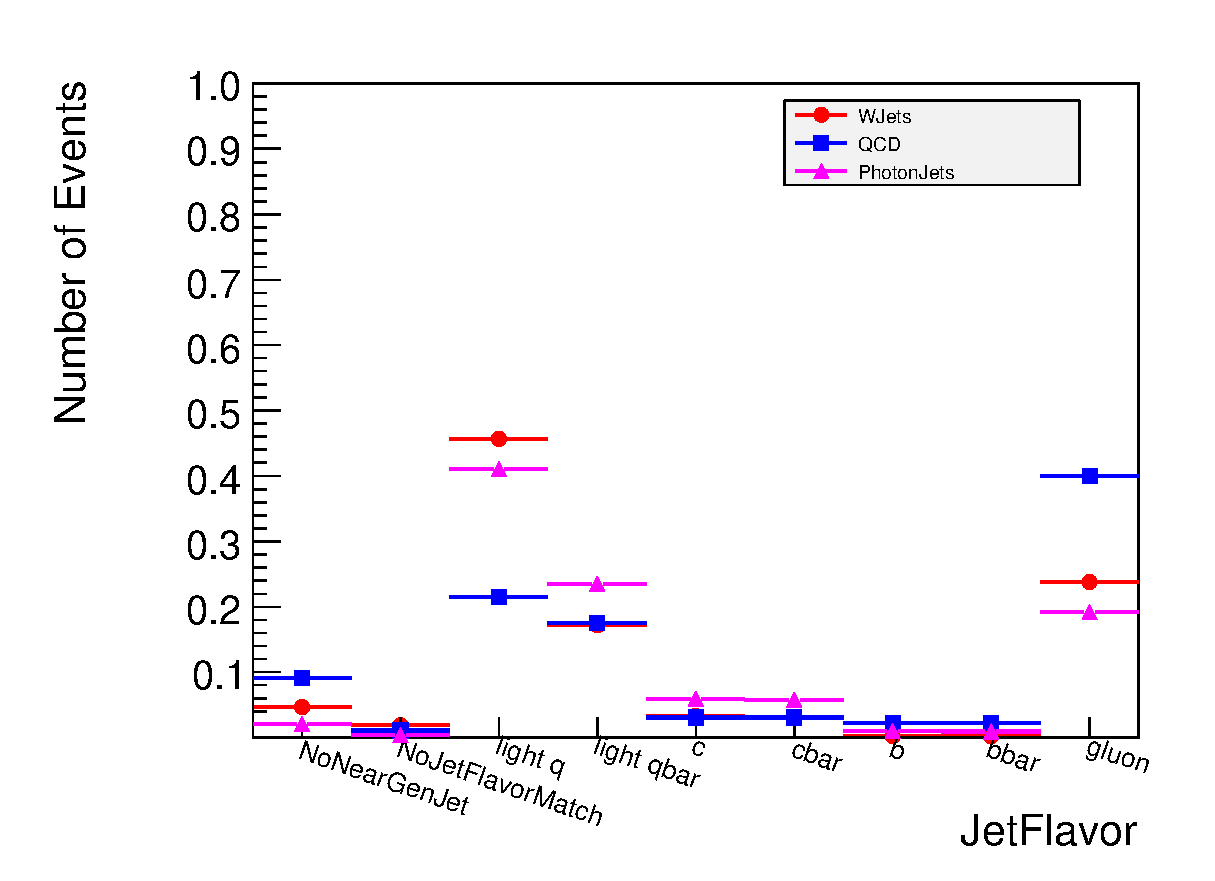
\includegraphics[width=0.49\textwidth]{plots/IsoTrackMuonDenominatorJetFlavor_Madgraph_WJetsVsQCD.eps}}    

   \caption{Fraction of fake muon isolated track denominators matched to the shown GenJet flavor. The color scheme is as in \FigureRef{fig:ElectronNumerator_FakeCategory}.}
   \label{fig:IsoTrackMuonDenominator_JetFlavor}
\end{center}
\end{figure}

\begin{figure}[htb]
\begin{center}
    \subfigure[]{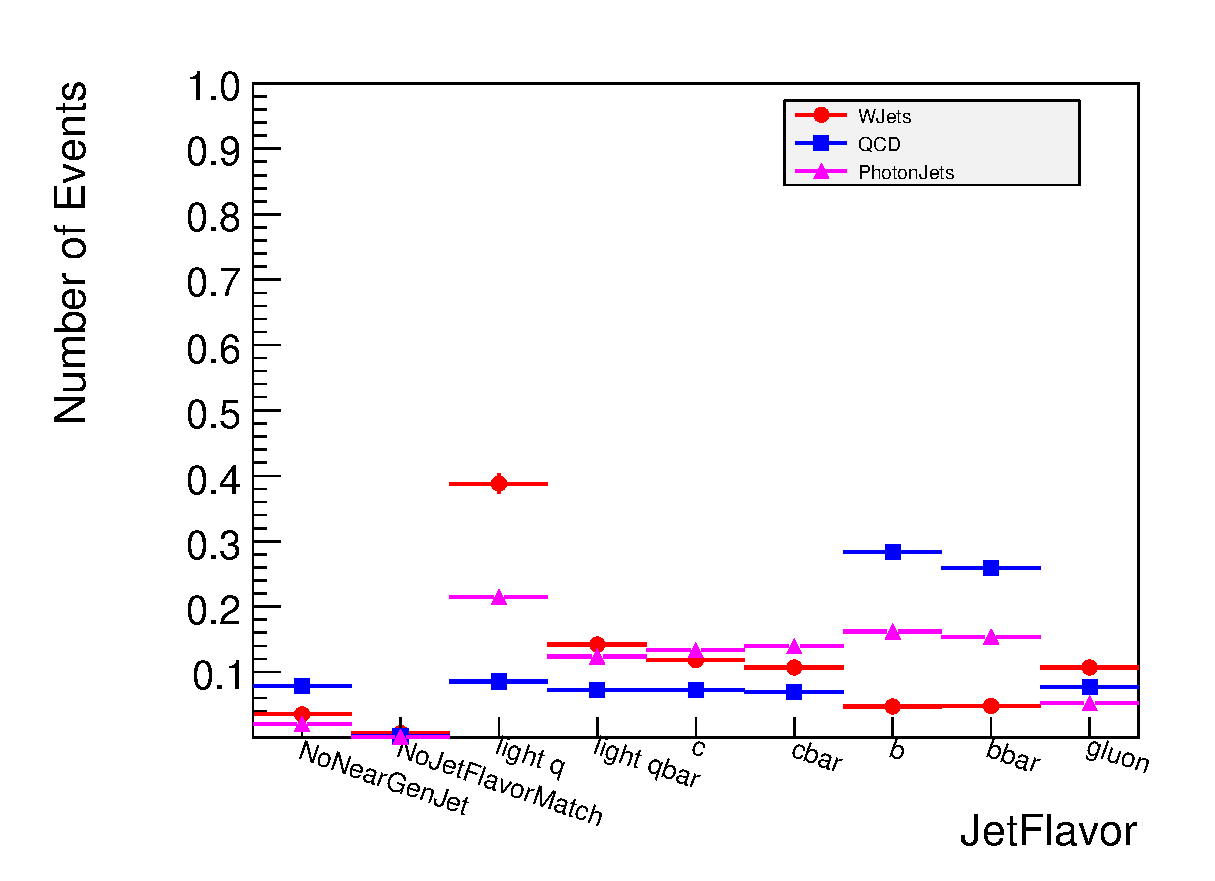
\includegraphics[width=0.49\textwidth]{plots/TrackerMuonDenominatorJetFlavor_Madgraph_WJetsVsQCD.eps}}
    \caption{Fraction of fake tracker muon denominators matched to the shown GenJet flavor. The color scheme is as in \FigureRef{fig:ElectronNumerator_FakeCategory}.}
   \label{fig:TrackerMuonDenominator_JetFlavor}
\end{center}
\end{figure}

\begin{figure}[htb]
\begin{center}
    \subfigure[]{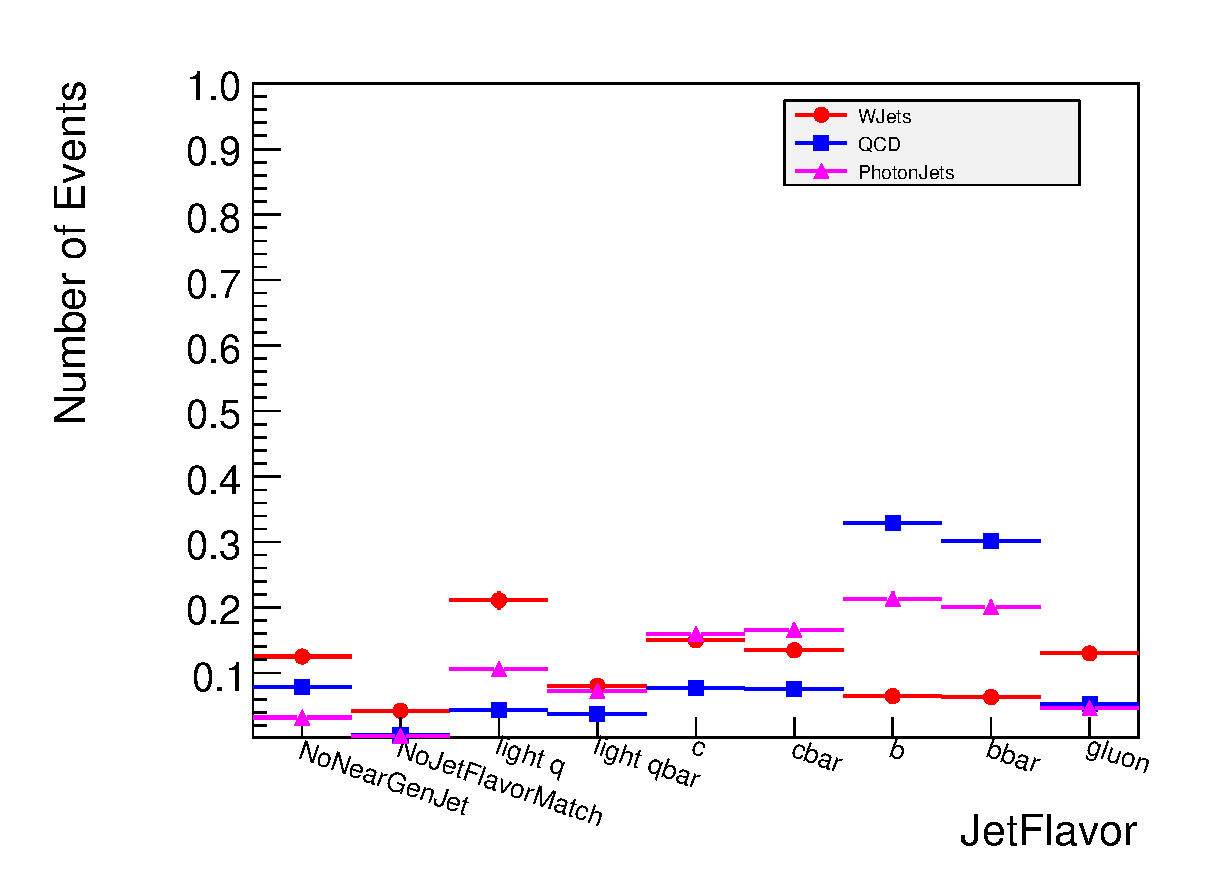
\includegraphics[width=0.49\textwidth]{plots/GlobalMuonDenominatorJetFlavor_Madgraph_WJetsVsQCD.eps}}
   \caption{Fraction of fake global muon denominators matched to the shown GenJet flavor. The color scheme is as in \FigureRef{fig:ElectronNumerator_FakeCategory}.}
   \label{fig:GlobalMuonDenominator_JetFlavor}
\end{center}
\end{figure}

The fake rates as a function of the matched jet flavor are shown in Figures~\ref{fig:IsoTrackMuonFakeRate_JetFlavor},~\ref{fig:TrackerMuonFakeRate_JetFlavor}, and~\ref{fig:GlobalMuonFakeRate_JetFlavor} for isolated track, tracker muon, and global muon denominators respectively. We see a clear difference in the fake rate for denominators matched to quarks versus denominators matched to gluons. The fake rate for gluon matched denominators is roughly one order of magnitude lower. 

\begin{figure}[htb]
\begin{center}
    \subfigure[]{\includegraphics[width=0.49\textwidth]{plots/IsoTrackMuonFakeRateJetFlavor_Madgraph_WJetsVsQCD.eps}}        
    \subfigure[]{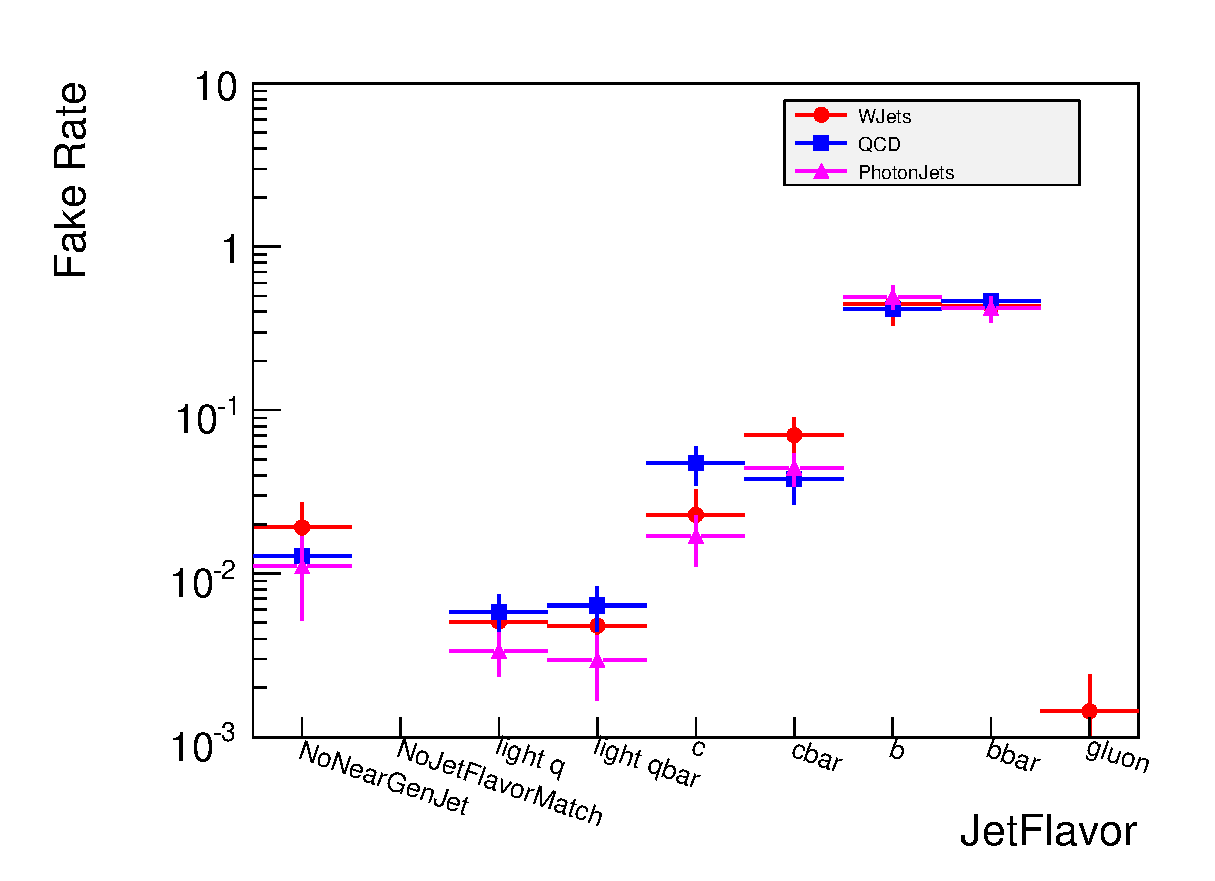
\includegraphics[width=0.49\textwidth]{plots/IsoTrackMuonFakeRateJetFlavor_Madgraph_WJetsVsQCD_logY.eps}}        
   \caption{The overall muon fake rate as a function of the matched GenJet Flavor for isolated track denominators shown in log scale. The color scheme is as in \FigureRef{fig:ElectronNumerator_FakeCategory}.}
   \label{fig:IsoTrackMuonFakeRate_JetFlavor}
\end{center}
\end{figure}

\clearpage

\begin{figure}[htb]
\begin{center}
    \subfigure[]{\includegraphics[width=0.49\textwidth]{plots/TrackerMuonFakeRateJetFlavor_Madgraph_WJetsVsQCD.eps}}    
    \subfigure[]{\includegraphics[width=0.49\textwidth]{plots/TrackerMuonFakeRateJetFlavor_Madgraph_WJetsVsQCD_logY.eps}}    
   \caption{The overall muon fake rate as a function of the matched GenJet Flavor for tracker muon denominators. The color scheme is as in \FigureRef{fig:ElectronNumerator_FakeCategory}.}
   \label{fig:TrackerMuonFakeRate_JetFlavor}
\end{center}
\end{figure}


\begin{figure}[htb]
\begin{center}
    \subfigure[]{\includegraphics[width=0.49\textwidth]{plots/GlobalMuonFakeRateJetFlavor_Madgraph_WJetsVsQCD.eps}}    
    \subfigure[]{\includegraphics[width=0.49\textwidth]{plots/GlobalMuonFakeRateJetFlavor_Madgraph_WJetsVsQCD_logY.eps}}    
   \caption{The overall muon fake rate as a function of the matched GenJet Flavor for global muon denominators. The color scheme is as in \FigureRef{fig:ElectronNumerator_FakeCategory}.}
   \label{fig:GlobalMuonFakeRate_JetFlavor}
\end{center}
\end{figure}

\customSection{Predictions for the Two Lepton Final State}
\begin{minipage}{\textwidth}
Using the fake rates shown above, we apply these two dimensional fake rates on the Fall08 Madgraph \WPlusJets\ Monte Carlo. More specifically, we use the following datasets:
\begin{itemize}
\item /WJets-madgraph/Summer08\_IDEAL\_V11\_redigi\_v1/GEN-SIM-RECO 
\item /VQQ-madgraph/Summer08\_IDEAL\_V11\_redigi\_v2/GEN-SIM-RECO 
\item /ZJets-madgraph/Summer08\_IDEAL\_V11\_redigi\_v1/GEN-SIM-RECO
\item /WW/Summer08\_IDEAL\_V11\_redigi\_v1/GEN-SIM-RECO
\item /TTJets-madgraph/Fall08\_IDEAL\_V11\_redigi\_v10/GEN-SIM-RECO
\end{itemize}

requiring, that the events contain one and only one lepton, plus any number of denominator objects.
\end{minipage}

In order to remove overlaps for the \W\ and \Z\ samples, we use the FlavorHistory tool \cite{FlavorHistory} to accept only matrix element \Wbb\ and \Wcc\ events where the b and bbar are sufficiently separated in $\Delta R$ ($\Delta R > 0.5$), and parton shower Wbb and Wcc events in the case where the \bottom and \bbar are close together ($\Delta R < 0.5$).

With this sample composition we compare the prediction of the two lepton final state from the fake rate method with the prediction made by the Monte Carlo simulation (subtracting those cases where both leptons are real). The $p_T$ and $\eta$ distributions of the fake electron and fake muon are shown in Figures~\ref{fig:fakeElectronPtEta} and \ref{fig:fakeMuonPtEta} respectively. The agreement is reasonably good. These plots are made after requiring two leptons with $p_T > 10.0$~GeV in the event.


\begin{figure}[htb]
  \begin{center}
    \subfigure[]{\includegraphics[width=0.49\textwidth]{plots/FakeElectronPt.eps}}
    \subfigure[]{\includegraphics[width=0.49\textwidth]{plots/FakeElectronEta.eps}}    
    \caption{The Pt (a) and Eta (b) distribution prediction for Fake Electrons in the two lepton final state, using the Fake Rate computed using the Reco denominator. The color  scheme is as in \FigureRef{fig:electronFakeRate_GsfTrack}.}
    \label{fig:fakeElectronPtEta}
  \end{center}
\end{figure}

\begin{figure}[htb]
  \begin{center}
    \subfigure[]{\includegraphics[width=0.49\textwidth]{plots/FakeMuonPt.eps}}
    \subfigure[]{\includegraphics[width=0.49\textwidth]{plots/FakeMuonEta.eps}}    
    \caption{The Pt (a) and Eta (b) distribution prediction for Fake Muons in the two lepton final state, using the tracker muon denominator. The color  scheme is as in \FigureRef{fig:electronFakeRate_GsfTrack}.}
    \label{fig:fakeMuonPtEta}
  \end{center}
\end{figure}


\customSubsection{\WPlusJets\ versus \WPlusGamma}
One subtlety that exists for the two lepton final state is that the background due to fake electrons are composed of both \WPlusJets\ events and \WPlusGamma\ events. The \WPlusGamma\ contribution introduces problems for predicting the charge correlation between the real lepton and the fake lepton. This effect will be discussed in greater detail in \SectionRef{sec:systematics_chargecorrelation}. To avoid this problem, we will use the fake rate method only for the background from \WPlusJets, while the \WPlusGamma\ background will be estimated using other methods.

However since these events will populate the extrapolation sample, one needs to properly remove them from the prediction. One possible method is to use the Monte Carlo simulation to predict the contribution from \WPlusGamma\ events to the extrapolation sample and subtract 
this contribution using negatively weighted events. For the current study we have removed events in the above samples which correspond to production of a photon 
with $p_T$ greater than $10~\GeVc$ at event generation level.

\customSubsection{Results}

In \FigureRef{fig:dileptonCharge}, we plot the distribution of the charge of the two leptons distinguishing the real lepton and the fake lepton, which shows reasonable agreement. This distribution is highly sensitive to the relative importance of the conversion fake category versus the charged hadron categories. The consequences of this effect are discussed further in \SectionRef{sec:systematics_chargecorrelation}.

\begin{figure}[htb]
\begin{center}
\includegraphics[width=0.49\textwidth]{plots/DileptonCharge.eps}
   \caption{The charge of the real lepton - fake lepton system. The four bins correspond to the case where both have positive charge (++), the real lepton has positive charge and the fake lepton has negative charge (+-), the real lepton has negative charge and the fake lepton has positive charge (-+) and both have negative charge (--). The color  scheme is as in \FigureRef{fig:electronFakeRate_GsfTrack}.}
   \label{fig:dileptonCharge}
\end{center}
\end{figure}

\begin{minipage}{\textwidth}
For the \WW\ and \HiggsToWW\ analyses, one is interested in the opposite sign events, while the same sign events are used as a control sample to validate the fake prediction. A few preselection cuts are made at this point:

\begin{itemize}
\item the leading lepton has $p_T > 20.0$~GeV,
\item the second lepton has $p_T > 10.0$~GeV,
\item there is no third lepton with $p_T > 10.0$~GeV, and
\item tThe two leptons with largest $p_T$ have opposite charge.
\end{itemize}
\end{minipage}

\begin{figure}[htb]
\begin{center}
    \subfigure[]{\includegraphics[width=0.49\textwidth]{plots/Lepton1Pt.eps}}
    \subfigure[]{\includegraphics[width=0.49\textwidth]{plots/Lepton2Pt.eps}}    
   \caption{The $p_T$ distribution for the leading lepton (a) and second lepton (b). The color  scheme is as in \FigureRef{fig:electronFakeRate_GsfTrack}.}
   \label{fig:leptonPt}
\end{center}
\end{figure}

\begin{figure}[htb]
\begin{center}
\includegraphics[width=0.85\textwidth]{plots/Met.eps}
   \caption{The missing transverse energy distribution. The color  scheme is as in \FigureRef{fig:electronFakeRate_GsfTrack}.}
   \label{fig:Met}
\end{center}
\end{figure}

\clearpage 

\FigureRef{fig:leptonPt} shows the $p_T$ distribution for the leading lepton and the second lepton in the opposite sign events, after the preselection. The comparison between the simulation and the prediction using the fake rate method is in reasonable agreement for both of these distributions. The missing transverse energy distribution is shown in \FigureRef{fig:Met}, and the difference in the $\phi$ coordinate between the two leptons and the invariant mass of the dilepton system are shown in \FigureRef{fig:deltaphi_dileptonMass}. All show reasonable agreement between the simulation and the predictions.


\begin{figure}[htb]
\begin{center}
    \subfigure[]{\includegraphics[width=0.49\textwidth]{plots/DeltaPhiLeptons.eps}}
    \subfigure[]{\includegraphics[width=0.49\textwidth]{plots/DileptonMass.eps}}    
   \caption{The distribution for the $\Delta\phi$ between the two leptons (a) and the invariant mass of the dilepton system (b) are shown. The color  scheme is as in \FigureRef{fig:electronFakeRate_GsfTrack}.}
   \label{fig:deltaphi_dileptonMass}
\end{center}
\end{figure}


\customSubsection{Contribution of non-\W\ Processes to the Prediction Sample}
There are a number of processes which contributes to the prediction sample in addition to \WPlusJets\ events. We show the contribution of each of the processes, in order to illustrate their relative importance. In \FigureRef{fig:leptonPtStacked_JetTriggerSample} we show the $p_T$ distribution of the first and second leptons from the prediction using the jet triggered sample. The prediction from the Monte Carlo simulation is overlayed for comparison. In \FigureRef{fig:leptonPtStacked_PhotonTriggerSample} we show the same distributions for the prediction using the photon triggered sample. One finds that the contribution from other processes, mainly Z+Jets, is relatively small.

\begin{figure}[htb]
  \begin{center}
    \subfigure[]{\includegraphics[width=0.49\textwidth]{plots/Lepton1Pt_Reco_TrackerMuon_Madgraph_Jet50.eps}}
    \subfigure[]{\includegraphics[width=0.49\textwidth]{plots/Lepton2Pt_Reco_TrackerMuon_Madgraph_Jet50.eps}}    
    \caption{The Pt of the first lepton (a) and the second lepton (b) separated by the underlying physics process, from the prediction using the jet triggered sample. The overlayed points show the prediction from the Monte Carlo simulation. }
    \label{fig:leptonPtStacked_JetTriggerSample}
  \end{center}
\end{figure}

\begin{figure}[htb]
  \begin{center}
    \subfigure[]{\includegraphics[width=0.49\textwidth]{plots/Lepton1Pt_Reco_TrackerMuon_Madgraph_Photon15.eps}}
    \subfigure[]{\includegraphics[width=0.49\textwidth]{plots/Lepton2Pt_Reco_TrackerMuon_Madgraph_Photon15.eps}}    
    \caption{The Pt of the first lepton (a) and the second lepton (b) separated by the underlying physics process, from the prediction using the photon triggered sample. The overlayed points show the prediction from the Monte Carlo simulation.}
    \label{fig:leptonPtStacked_PhotonTriggerSample}
  \end{center}
\end{figure}

One subtlety exists for processes containing two real leptons, in particular Z and \TTBAR. When one of the real leptons fails lepton identification cuts, that event will enter the extrapolation sample. It will receive a weight based on the fake rate functions and will be added to the fake background prediction. This is an incorrect addition to the background prediction, since such events is already accounted for by the Monte Carlo based background estimate. In data, we must subtract the Z and \TTBAR events for which one of the real leptons failed lepton identification from the extrapolation sample. The amount to be subtracted will be obtained from the Monte Carlo prediction. This subtraction has been done in the plots shown above.


\customSubsection{Estimation of Systematic Uncertainties}
The underlying issue that dominates systematic uncertainties in this method is the uncertainty on the sample composition of the calibration sample and the extrapolation sample. Since different fake processes have different values of \epsilonFake, the relative importance of each fake process is a large factor in determining the overall value of \epsilonFake~that one should apply to obtain an accurate prediction. We discuss a number of methods that can be studied in data to derive an estimate of the systematic uncertainty on the fake lepton background prediction, and present some simple results based on the Monte Carlo simulation.

Having identified the main processes responsible for electron and muon fakes, one can try to use particular cuts to enhance specific processes. One can then measure \epsilonFake~in these process enhanced samples in order to obtain some bounds on the true \epsilonFake~value in the extrapolation sample. To give an example, for muons one can require a b-tag on the trigger jet and measure \epsilonFake~in this heavy flavor enhanced sample. Another example is to measure \epsilonFake~in a sample enhanced in conversions by requiring that a conversion candidate is found with one leg matching to the denominator. A reasonable estimate of the systematic uncertainties can be derived after one has obtained reasonable bounds on the true \epsilonFake~value in the extrapolation sample. This method requires comprehensive study of all the fake processes, but gives greater confidence in our results.

Another method to derive or to constrain the systematic uncertainties is to apply the method for predicting the final state containing two same sign leptons. In this final state, assuming that there is no new physics populating this final state, one expects purely fake leptons. By comparing the prediction from various calibration samples with the data, one can obtain an estimate of the systematic uncertainties by looking for the largest deviation between the prediction and the data. This final state can also be used together with other methods to help constrain the systematic uncertainties more.

Finally, one can compare the fake lepton background prediction of this method with the prediction of a completely independant method. Differences in the predictions can give very rough bounds on the size of the systematic uncertainties. However, since different methods have intrinsically different underlying systematic issues, one must be careful not to make ill defined comparisons.

The method which we will present in this note is to compare the \epsilonFake~measurements in the different calibration samples and the extrapolation sample. One half of the largest difference between any two measurements will be taken as the systematic uncertainty on the \epsilonFake~measurement. The correctness of this estimate depends on the implicit assumption that the true \epsilonFake value of the extrapolation sample in data is within the difference of these measurements. Clearly this assumption requires justification, which is beyond the scope of this current study.  Another related method is to use the difference of the \epsilonFake~measurement in samples derived from different jet triggers. 

\begin{figure}[htb]
  \begin{center}
    \subfigure[]{\includegraphics[width=0.49\textwidth]{plots/RecoElectronFakeRatePt_WithSystematics.eps}}
    \subfigure[]{\includegraphics[width=0.49\textwidth]{plots/RecoElectronFakeRateEta_WithSystematics.eps}}    
    \caption{The measurement of \epsilonFake for electrons using the Reco denominator in the jet triggered sample with systematic uncertainties versus $p_T$ in (a) and $\eta$ in (b). Comparison to the measurement in the \WPlusJets\ simulation and the photon triggered sample is shown. The color  scheme is as in \FigureRef{fig:electronFakeRate_GsfTrack}.}
    \label{fig:electronFakeRate_WithSystematics}
  \end{center}
\end{figure}

\begin{figure}[htb]
  \begin{center}
    \subfigure[]{\includegraphics[width=0.49\textwidth]{plots/TrackerMuonFakeRatePt_WithSystematics.eps}}
    \subfigure[]{\includegraphics[width=0.49\textwidth]{plots/TrackerMuonFakeRateEta_WithSystematics.eps}}    
    \caption{The measurement of \epsilonFake for muons using the tracker muon denominator in the jet triggered sample with systematic uncertainties versus $p_T$ in (a) and $\eta$ in (b). Comparison to the measurement in the \WPlusJets\ simulation and the photon triggered sample is shown. The color  scheme is as in \FigureRef{fig:electronFakeRate_GsfTrack}.}
    \label{fig:muonFakeRate_WithSystematics}
  \end{center}
\end{figure}

In the current study, we present systematic uncertainties derived from the difference of measurements in the different samples as measured in Monte Carlo simulation. In Figures~\ref{fig:electronFakeRate_WithSystematics} and \ref{fig:muonFakeRate_WithSystematics} we show the one dimensional projections for the \epsilonFake value for electrons and muons measured in the jet triggered sample with the systematic uncertainties represented by the shaded region. These plots show that the procedure performed in Monte Carlo simulation gives systematic uncertainties of roughly 30\%.

In \FigureRef{fig:DeltaPhiDileptonMass_WithSystematics}, we show the distribution of the $\Delta\phi$ between the two leptons and the dilepton mass with systematic uncertainties propagated to the prediction. The uncertainties shown are computed by adding the statistical uncertainty, the systematic uncertainty as described above, and the Monte Carlo statistical uncertainty from the \epsilonFake~measurement all in quadrature. Finally, in \FigureRef{fig:HWWSelection_WithSystematics}, we show the number of events left in the fake lepton background processes after each cut in the \HiggsToWW\ analysis for a Higgs mass of 160GeV. The final prediction for the fake lepton backgrounds using this method in Monte Carlo are $0.4\pm0.2$ events in $200\ipb$. This prediction gives a rough idea to illustrate the performance of the method; the final prediction will be obtained using collision data.

\begin{figure}[htb]
  \begin{center}
    \subfigure[]{\includegraphics[width=0.49\textwidth]{plots/DeltaPhiLeptons_withSysError.eps}}
    \subfigure[]{\includegraphics[width=0.49\textwidth]{plots/DileptonMass_withSysError.eps}}    
    \caption{The distribution for the $\Delta\phi$ between the two leptons (a) and the invariant mass of the dilepton system (b) with systematic uncertainties. The shaded region represents the systematic uncertainties, centered on the prediction from the jet triggered sample measurement. The prediction from the Monte Carlo simulation and the photon triggered sample are shown for comparison. The color  scheme is as in \FigureRef{fig:electronFakeRate_GsfTrack}.}
    \label{fig:DeltaPhiDileptonMass_WithSystematics}
  \end{center}
\end{figure}

\begin{figure}[htb]
  \begin{center}
    \subfigure[]{\includegraphics[width=\textwidth]{plots/HWWSelection_withSysError_logY.eps}}
    \caption{The number of events remaining for fake lepton processes after each cut for the \HiggsToWW\ analysis. Systematic uncertainties on the prediction from the jet triggered sample are shown in the shaded region. The prediction from the Monte Carlo simulation and the photon triggered sample are shown for comparison. The exact definition of the cuts are given in \TableRef{tab:HWWCuts}. The color  scheme is as in \FigureRef{fig:electronFakeRate_GsfTrack}.}
    \label{fig:HWWSelection_WithSystematics}
  \end{center}
\end{figure}

\begin{table}[ht]
  \begin{center}
    \footnotesize  
    \begin{tabular}{|c|c|}\hline 
      Cut Label & Cut Definition \\ 
      \hline 
      PreSel & Lepton1 $p_T > 20.0$~GeV \& Lepton2 $p_T > 10.0$~GeV \& $\met > 30.0$~GeV \& $\mll > 12.0$~GeV \\ 
      CJVeto & No Jets with $|\eta| < 2.5$ \\ 
      MetCut & $\met > 50.0$~GeV \& $\met < 200.0$~GeV \\ 
      $\Delta\phi$Cut &  $\delphill < 45$~degrees \\ 
      MassCut & $\mll < 50.0$~GeV \\ 
      Pt1Cut & Lepton1 $p_T > 35.0$~GeV \& Lepton1 $p_T < 55.0$~GeV \\ 
      Pt2Cut & Lepton2 $p_T > 25.0$~GeV  \\ 
      MuonVeto & No additional non-isolated muons\\ 
      NTracksCut & Number of additional tracks (with $p_T > 3.0$~GeV) $ < 4$ \\ 
      \hline 
    \end{tabular}         
  \end{center}
  \caption{\label{tab:HWWCuts} Exact definitions of the cuts for the \HiggsToWW\ analysis ($m_{H} = 160$~GeV) shown in \FigureRef{fig:HWWSelection_WithSystematics}. }
\end{table}




\customSection{Conclusions}
The fake rate method for estimating backgrounds of processes involving a fake lepton has been presented. Measurements of the \epsilonFake value for electrons and muons have been performed in the jet triggered sample and the photon triggered sample. A number of denominator definitions have been studied. For electrons the best performing denominator is the Reco denominator, while for muons the tracker muon denominator is most appropriate. Variations of roughly 30\% are found for the measurements in the different samples.

A number of systematic effects such as sample composition and jet flavor dependance have been studied in detail using the Monte Carlo simulation. Algorithms to classify different lepton fake processes in simulation have been created and validated. As a result of these studies, a number of issues affecting systematic unknowns have been identified for further study in data.

Finally, the method was used to predict the fake lepton background for the two lepton final state and validated with comparisons to the Monte Carlo simulation. A reasonable agreement is observed for various kinematic distributions and cut variables relevent for the \WW\ and \HiggsToWW\ analyses. The method predicts 0.4$ \pm 0.2\mathrm{(systematic\ uncertainty)}$ events for $200\ipb$ of data for the Higgs analysis after all cuts.

\pagebreak

\vspace*{-0.2cm}
\thebibliography{12}

\bibitem{fakeLeptonNote}
CMS AN-2009/041, ``Data-driven methods to estimate the electron and muon fake contributions to lepton analyses'',
O. Gutsche \textit{et al.}.

\bibitem{CDFTopDilepton}
T. Aaltonen et al., The CDF Collaboration, Fermilab-Pub-09-091-E. arXiv:0903.5263.

\bibitem{electronID}
CMS AN-2008/082, ``A cut based method for electron identification in CMS'',
J. Branson \textit{et al.}.

\bibitem{jurassicIsolation}
http://indico.cern.ch/getFile.py/access?contribId=1\&resId=0\&materialId=slides\&confId=27568

\bibitem{muonID}
CMS AN-2008/098, ``Muon Identification in CMS'',
M. Mulders \textit{et al.}.

\bibitem{HLTTable}
https://twiki.cern.ch/twiki/bin/view/CMS/TSG\_17\_X\_08 

\bibitem{PhotonID}
https://twiki.cern.ch/twiki/bin/view/CMS/PhotonIDAnalysis

\bibitem{JetEnergyCalibrationWithPhotonJet}
CMS AN-2009/012, ``Jet energy calibration with photon+jet events'',
Daniele del Re, Mikko Voutilainen.

\bibitem{FlavorHistory}
https://twiki.cern.ch/twiki/bin/view/CMS/SWGuideFlavorHistory
\newpage

\clearpage
\appendix 

\customSection{Conversion Veto} 
\label{app:conversionveto}
For identifying conversions we use a vertex fitting procedure applying a constraint on the angle between the conversion legs at the vertex. Conversion candidates are formed by vertexing a Gsf track with a regular track. The following cuts are applied on the conversion candidates to reduce fake conversion background:

\begin{itemize}
\item Conversion Fit Probility $> 0.0005$,
\item $L_{xy} > 0$, and
\item $L_z > 0$.
\end{itemize}

Furthermore, the leg of the conversion that is a regular track must pass the following cuts:
\begin{itemize}
\item $N_{Hits}~>~0$,
\item track Probability $ > 0.005$, and
\item the track contains no hits that project to a location behind the vertex, where some allowance is made to account for the uncertainty in the vertex resolution.
\end{itemize}

If the Gsf track of the electron candidate is one leg of a conversion passing all of the above cuts, then the electron candidate is rejected.

\customSection{Trigger Correction to \epsilonFake} 
\label{app:triggerCorrection}
For identifying conversions we use a vertex fitting procedure applying a constraint on the angle between the conversion legs at the vertex. Conversion candidates are formed by vertexing a Gsf track with a regular track. The following cuts are applied on the conversion candidates to reduce fake conversion background:
The trigger correction is required because the probability for a real lepton to fail the HLT requirement and for the fake denominator to fire the HLT is small. However the probability for this to occur is not small if the fake denominator is known to pass offline tight lepton cuts. These events do not enter the extrapolation sample, because they do not fire any lepton trigger, and therefore are missing from the prediction.

This can be seen by considering the limit in which \epsilonFake~ $\approx 1$. Then we have:
\begin{eqnarray}
  N^{app}_{\textrm{HLT fired}}\frac{\epsilonFake}{1-\epsilonFake} & = & N^{app}_{\textrm{l fires HLT}}\frac{\epsilonFake}{1-\epsilonFake} + N^{app}_{\textrm{l fails HLT \& d fires HLT}}\frac{\epsilonFake}{1-\epsilonFake} \nonumber \\
 & = & N^{sig}_{\textrm{l fires HLT}} + N^{sig}_{\textrm{l fails HLT \& f fires HLT}}
\end{eqnarray}
so that the first term already gives the correction contribution automatically. 

Note that this is not true if \epsilonFake~is small because in order for the final equality to hold for the second term, the \epsilonFake~value that one needs to apply is the efficiency for a denominator which fired the HLT to pass numerator cuts. This value is close to the value that is measured in the calibration sample only when the denominator is sufficiently tight that the requirement for it to fire the HLT does not introduce a bias.

One could measure the \epsilonFake~values separately for cases where denominators fire the HLT, however this introduces additional complications and it is likely that one does not have enough data events to perform these separate measurements of \epsilonFake.

\customSection{Two Dimensional Electron Fake Rates}
\label{app:electronfakerates}

One dimensional slices in $p_T$ and $\eta$ of the electron fake rate are shown in Figures~\ref{fig:electronFR_gsftrack_etaslices},~\ref{fig:electronFR_gsftrack_ptslices},~\ref{fig:electronFR_reco_etaslices} 
and~\ref{fig:electronFR_reco_ptslices}.

\begin{figure}[htb]
\begin{center}
\includegraphics[width=0.98\textwidth]{plots/GsfTrackElectronFakeRateEtaSlices.eps}
   \caption{Electron fake rate as a function of $p_T$ for various $\eta$ slices for the GsfTrack denominator definition. }
   \label{fig:electronFR_gsftrack_etaslices}
\end{center}
\end{figure}

\begin{figure}[htb]
\begin{center}
\includegraphics[width=0.98\textwidth]{plots/GsfTrackElectronFakeRatePtSlices.eps}
   \caption{Electron fake rate as a function of $\eta$ for various $p_T$ slices for the GsfTrack denominator definition. }
   \label{fig:electronFR_gsftrack_ptslices}
\end{center}
\end{figure}

\begin{figure}[htb]
\begin{center}
\includegraphics[width=0.98\textwidth]{plots/RecoElectronFakeRateEtaSlices.eps}
   \caption{Electron fake rate as a function of $p_T$ for various $\eta$ slices for the RecoElectron denominator definition. }
   \label{fig:electronFR_reco_etaslices}
\end{center}
\end{figure}

\begin{figure}[htb]
\begin{center}
\includegraphics[width=0.98\textwidth]{plots/RecoElectronFakeRatePtSlices.eps}
   \caption{Electron fake rate as a function of $\eta$ for various $p_T$ slices for the RecoElectron denominator definition. }
   \label{fig:electronFR_reco_ptslices}
\end{center}
\end{figure}

The full two-dimensional fake rates are given in Tables~\ref{tab:electronFR_gsftrack_wjets},~\ref{tab:electronFR_gsftrack_JetTriggerSample}, and~\ref{tab:electronFR_gsftrack_PhotonTriggerSample} for GsfTrack denominators and in Tables~\ref{tab:electronFR_reco_wjets},~\ref{tab:electronFR_reco_JetTriggerSample}, and~\ref{tab:electronFR_reco_PhotonTriggerSample} for Reco denominators. We show the fake rates measured in the \WPlusJets\ Monte Carlo sample, the JetTrigger sample (HLT\_Jet50), and the photon triggered sample (HLT\_Photon15).

\begin{table}[ht]
  \begin{center}
    \large 
GsfTrack Denominator Fake Rate for the W+Jets sample
\footnotesize 
\begin{tabular*}{\textwidth}{|c|c|c|c|c|c|c|c|}\hline 
$p_T$ [GeV/c] / $\eta$  & -2.75 To -2.25 & -2.25 To -1.75 & -1.75 To -1.25 & -1.25 To -0.75 & -0.75 To -0.25 & -0.25 To 0.25 & 0.25 To 0.75 \\ 
 \hline 
0.0 - 10.0 & 0.000e+00 & 0.000e+00 & 0.000e+00 & 0.000e+00 & 0.000e+00 & 0.000e+00 & 0.000e+00 \\ 
10.0 - 15.0 & 3.994e-03 & 1.721e-03 & 1.725e-03 & 2.723e-03 & 4.403e-04 & 1.296e-03 & 1.352e-03 \\ 
15.0 - 20.0 & 1.223e-02 & 3.987e-03 & 4.963e-03 & 5.416e-03 & 5.288e-05 & 8.821e-04 & 4.603e-03 \\ 
20.0 - 25.0 & 1.469e-02 & 8.148e-03 & 1.033e-02 & 8.442e-03 & 4.896e-03 & 4.469e-03 & 4.690e-03 \\ 
25.0 - 30.0 & 8.877e-03 & 1.570e-02 & 2.048e-02 & 4.646e-03 & 8.048e-03 & 5.336e-03 & 9.705e-03 \\ 
30.0 - 35.0 & 2.950e-02 & 3.027e-02 & 5.500e-03 & 3.026e-02 & 1.429e-02 & 0.000e+00 & 1.032e-02 \\ 
35.0 - 40.0 & 3.031e-02 & 3.078e-02 & 1.687e-02 & 3.900e-02 & 2.712e-02 & 6.351e-03 & 5.891e-03 \\ 
40.0 - 50.0 & 7.934e-03 & 6.474e-03 & 0.000e+00 & 2.374e-02 & 6.069e-03 & 0.000e+00 & 2.274e-02 \\ 
50.0 - 80.0 & 4.097e-02 & 2.513e-02 & 0.000e+00 & 9.480e-03 & 0.000e+00 & 1.931e-02 & 1.258e-02 \\ 
80.0 - 120.0 & 0.000e+00 & 0.000e+00 & 0.000e+00 & 0.000e+00 & 0.000e+00 & 0.000e+00 & 0.000e+00 \\ 
120.0 - 170.0 & 0.000e+00 & 0.000e+00 & 0.000e+00 & 0.000e+00 & 0.000e+00 & 0.000e+00 & 0.000e+00 \\ 
170.0 - 250.0 & 0.000e+00 & 0.000e+00 & 0.000e+00 & 0.000e+00 & 0.000e+00 & 0.000e+00 & 0.000e+00 \\ 
 \hline 
\end{tabular*} 
\begin{tabular}{|c|c|c|c|c|}\hline 
$p_T$ [GeV/c] / $\eta$  & 0.75 To 1.25 & 1.25 To 1.75 & 1.75 To 2.25 & 2.25 To 2.75 \\ 
 \hline 
0.0 - 10.0 & 0.000e+00 & 0.000e+00 & 0.000e+00 & 0.000e+00 \\ 
10.0 - 15.0 & 3.091e-03 & 1.170e-03 & 2.639e-03 & 2.243e-03 \\ 
15.0 - 20.0 & 4.259e-03 & 5.451e-03 & 1.585e-02 & 5.307e-03 \\ 
20.0 - 25.0 & 8.719e-03 & 1.182e-02 & 1.101e-02 & 7.399e-03 \\ 
25.0 - 30.0 & 1.639e-02 & 1.726e-02 & 3.297e-02 & 2.271e-02 \\ 
30.0 - 35.0 & 9.403e-03 & 2.068e-02 & 2.345e-02 & 2.008e-02 \\ 
35.0 - 40.0 & 1.592e-02 & 1.398e-02 & 8.650e-03 & 6.150e-02 \\ 
40.0 - 50.0 & 1.977e-02 & 7.497e-03 & 2.659e-02 & 9.185e-03 \\ 
50.0 - 80.0 & 1.459e-02 & 1.576e-02 & 2.387e-02 & 2.010e-02 \\ 
80.0 - 120.0 & 0.000e+00 & 0.000e+00 & 0.000e+00 & 1.041e-01 \\ 
120.0 - 170.0 & 0.000e+00 & 1.667e-01 & 0.000e+00 & 0.000e+00 \\ 
170.0 - 250.0 & 0.000e+00 & 0.000e+00 & 0.000e+00 & 0.000e+00 \\ 
 \hline 
\end{tabular} 

  \end{center}
  \caption{\label{tab:electronFR_gsftrack_wjets} Electron fake rates as a function of $p_T$ and $\eta$ for the GsfTrack denominator measured in the \WPlusJets\ sample.}
\end{table}

\begin{table}[ht]
  \begin{center}
    \large 
GsfTrack Denominator Fake Rate for the JetTrigger sample
\footnotesize 
\begin{tabular*}{\textwidth}{|c|c|c|c|c|c|c|c|}\hline 
$p_T$ [GeV/c] / $\eta$  & -2.75 To -2.25 & -2.25 To -1.75 & -1.75 To -1.25 & -1.25 To -0.75 & -0.75 To -0.25 & -0.25 To 0.25 & 0.25 To 0.75 \\ 
 \hline 
0.0 - 10.0 & 0.000e+00 & 0.000e+00 & 0.000e+00 & 0.000e+00 & 0.000e+00 & 0.000e+00 & 0.000e+00 \\ 
10.0 - 15.0 & 2.015e-03 & 1.395e-03 & 8.774e-04 & 2.062e-03 & 1.077e-03 & 6.602e-04 & 9.780e-04 \\ 
15.0 - 20.0 & 4.018e-03 & 5.902e-03 & 4.016e-03 & 4.132e-03 & 3.326e-03 & 1.994e-03 & 3.256e-03 \\ 
20.0 - 25.0 & 7.165e-03 & 1.044e-02 & 1.120e-02 & 8.738e-03 & 4.666e-03 & 5.661e-03 & 6.114e-03 \\ 
25.0 - 30.0 & 8.601e-03 & 1.557e-02 & 1.655e-02 & 5.416e-03 & 1.186e-02 & 3.111e-03 & 7.510e-03 \\ 
30.0 - 35.0 & 1.302e-02 & 1.375e-02 & 1.865e-02 & 1.039e-02 & 5.747e-03 & 7.226e-03 & 8.707e-03 \\ 
35.0 - 40.0 & 1.346e-02 & 1.582e-02 & 1.928e-02 & 1.478e-02 & 1.114e-02 & 4.318e-03 & 5.858e-03 \\ 
40.0 - 50.0 & 1.008e-02 & 1.637e-02 & 2.124e-02 & 5.067e-03 & 2.652e-03 & 1.869e-03 & 6.342e-03 \\ 
50.0 - 80.0 & 1.601e-02 & 1.763e-02 & 8.115e-03 & 6.426e-03 & 4.082e-03 & 3.449e-03 & 4.775e-03 \\ 
80.0 - 120.0 & 1.762e-02 & 1.696e-02 & 1.448e-02 & 7.905e-03 & 1.132e-02 & 1.233e-02 & 8.057e-03 \\ 
120.0 - 170.0 & 1.271e-02 & 1.739e-02 & 1.374e-02 & 9.448e-03 & 4.020e-03 & 5.889e-03 & 5.970e-03 \\ 
170.0 - 250.0 & 3.117e-03 & 1.995e-02 & 1.066e-02 & 1.257e-02 & 7.986e-03 & 5.382e-03 & 4.958e-03 \\ 
 \hline 
\end{tabular*} 
\begin{tabular}{|c|c|c|c|c|}\hline 
$p_T$ [GeV/c] / $\eta$  & 0.75 To 1.25 & 1.25 To 1.75 & 1.75 To 2.25 & 2.25 To 2.75 \\ 
 \hline 
0.0 - 10.0 & 0.000e+00 & 0.000e+00 & 0.000e+00 & 0.000e+00 \\ 
10.0 - 15.0 & 1.434e-03 & 1.035e-03 & 1.648e-03 & 2.396e-03 \\ 
15.0 - 20.0 & 3.981e-03 & 2.624e-03 & 4.192e-03 & 2.983e-03 \\ 
20.0 - 25.0 & 8.751e-03 & 1.063e-02 & 1.058e-02 & 6.890e-03 \\ 
25.0 - 30.0 & 1.265e-02 & 1.168e-02 & 1.250e-02 & 9.143e-03 \\ 
30.0 - 35.0 & 1.501e-02 & 1.515e-02 & 1.992e-02 & 1.441e-02 \\ 
35.0 - 40.0 & 2.321e-02 & 1.533e-02 & 1.851e-02 & 1.827e-02 \\ 
40.0 - 50.0 & 9.817e-03 & 2.228e-02 & 1.513e-02 & 1.375e-02 \\ 
50.0 - 80.0 & 1.843e-02 & 3.811e-02 & 3.054e-02 & 1.148e-02 \\ 
80.0 - 120.0 & 1.231e-02 & 1.214e-02 & 2.008e-02 & 1.045e-02 \\ 
120.0 - 170.0 & 9.796e-03 & 1.088e-02 & 1.626e-02 & 9.470e-03 \\ 
170.0 - 250.0 & 9.802e-03 & 9.975e-03 & 1.717e-02 & 2.973e-03 \\ 
 \hline 
\end{tabular} 

  \end{center}
  \caption{\label{tab:electronFR_gsftrack_JetTriggerSample} Electron fake rates as a function of $p_T$ and $\eta$ for the GsfTrack denominator measured in the Jet Triggered sample (HLT\_Jet50).}
\end{table}

\begin{table}[ht]
  \begin{center}
    \large 
GsfTrack Denominator Fake Rate for the PhotonTrigger sample
\footnotesize 
\begin{tabular*}{\textwidth}{|c|c|c|c|c|c|c|c|}\hline 
$p_T$ [GeV/c] / $\eta$  & -2.75 To -2.25 & -2.25 To -1.75 & -1.75 To -1.25 & -1.25 To -0.75 & -0.75 To -0.25 & -0.25 To 0.25 & 0.25 To 0.75 \\ 
 \hline 
0.0 - 10.0 & 0.000e+00 & 0.000e+00 & 0.000e+00 & 0.000e+00 & 0.000e+00 & 0.000e+00 & 0.000e+00 \\ 
10.0 - 15.0 & 3.329e-03 & 2.338e-03 & 1.545e-03 & 1.523e-03 & 1.785e-03 & 2.293e-03 & 3.956e-04 \\ 
15.0 - 20.0 & 7.179e-03 & 5.500e-03 & 9.097e-03 & 7.683e-03 & 5.566e-03 & 2.366e-03 & 5.114e-03 \\ 
20.0 - 25.0 & 1.502e-02 & 1.433e-02 & 1.702e-02 & 4.280e-03 & 4.466e-03 & 5.621e-03 & 6.920e-03 \\ 
25.0 - 30.0 & 2.265e-02 & 1.418e-02 & 2.540e-02 & 4.430e-03 & 8.368e-03 & 1.053e-02 & 2.532e-03 \\ 
30.0 - 35.0 & 1.985e-02 & 4.000e-02 & 3.007e-02 & 1.863e-02 & 4.949e-03 & 2.825e-02 & 8.687e-03 \\ 
35.0 - 40.0 & 2.593e-02 & 2.195e-02 & 3.417e-02 & 2.235e-02 & 2.012e-02 & 1.118e-02 & 3.902e-03 \\ 
40.0 - 50.0 & 4.599e-02 & 4.885e-02 & 5.517e-02 & 1.501e-02 & 4.402e-03 & 3.408e-04 & 7.772e-03 \\ 
50.0 - 80.0 & 7.462e-02 & 1.825e-02 & 6.975e-02 & 2.453e-02 & 6.230e-03 & 1.066e-02 & 1.149e-02 \\ 
80.0 - 120.0 & 1.105e-02 & 9.199e-02 & 1.300e-02 & 3.104e-03 & 5.903e-03 & 5.644e-03 & 8.602e-02 \\ 
120.0 - 170.0 & 8.547e-03 & 1.843e-02 & 1.176e-02 & 4.608e-03 & 5.196e-03 & 6.473e-03 & 7.092e-03 \\ 
170.0 - 250.0 & 0.000e+00 & 1.818e-02 & 5.970e-02 & 1.695e-02 & 1.408e-02 & 1.562e-02 & 1.449e-02 \\ 
 \hline 
\end{tabular*} 
\begin{tabular}{|c|c|c|c|c|}\hline 
$p_T$ [GeV/c] / $\eta$  & 0.75 To 1.25 & 1.25 To 1.75 & 1.75 To 2.25 & 2.25 To 2.75 \\ 
 \hline 
0.0 - 10.0 & 0.000e+00 & 0.000e+00 & 0.000e+00 & 0.000e+00 \\ 
10.0 - 15.0 & 3.214e-03 & 1.637e-04 & 9.645e-04 & 7.605e-04 \\ 
15.0 - 20.0 & 4.677e-03 & 4.856e-03 & 8.675e-03 & 4.662e-03 \\ 
20.0 - 25.0 & 1.133e-02 & 1.213e-02 & 2.253e-02 & 2.367e-02 \\ 
25.0 - 30.0 & 1.345e-02 & 2.013e-02 & 3.124e-02 & 2.733e-02 \\ 
30.0 - 35.0 & 2.718e-02 & 2.852e-02 & 4.641e-02 & 2.958e-02 \\ 
35.0 - 40.0 & 2.607e-02 & 3.107e-02 & 2.795e-02 & 1.994e-02 \\ 
40.0 - 50.0 & 1.716e-02 & 5.365e-02 & 4.496e-02 & 3.726e-02 \\ 
50.0 - 80.0 & 1.213e-02 & 5.051e-02 & 2.363e-02 & 4.152e-02 \\ 
80.0 - 120.0 & 1.174e-02 & 1.148e-02 & 1.268e-02 & 2.473e-03 \\ 
120.0 - 170.0 & 7.843e-03 & 0.000e+00 & 2.974e-02 & 0.000e+00 \\ 
170.0 - 250.0 & 5.797e-02 & 3.774e-02 & 3.226e-02 & 0.000e+00 \\ 
 \hline 
\end{tabular} 

  \end{center}
  \caption{\label{tab:electronFR_gsftrack_PhotonTriggerSample} Electron fake rates as a function of $p_T$ and $\eta$ for the GsfTrack denominator measured in the photon triggered sample (HLT\_Photon15).}
\end{table}

\begin{table}[ht]
  \begin{center}
    \large 
Reco Denominator Fake Rate for the W+Jets sample
\footnotesize 
\begin{tabular*}{\textwidth}{|c|c|c|c|c|c|c|c|}\hline 
$p_T$ [GeV/c] / $\eta$  & -2.75 To -2.25 & -2.25 To -1.75 & -1.75 To -1.25 & -1.25 To -0.75 & -0.75 To -0.25 & -0.25 To 0.25 & 0.25 To 0.75 \\ 
 \hline 
0.0 - 10.0 & 0.000e+00 & 0.000e+00 & 0.000e+00 & 0.000e+00 & 0.000e+00 & 0.000e+00 & 0.000e+00 \\ 
10.0 - 15.0 & 1.384e-02 & 4.447e-03 & 2.070e-03 & 3.159e-03 & 6.332e-04 & 1.969e-03 & 1.874e-03 \\ 
15.0 - 20.0 & 4.439e-02 & 1.139e-02 & 8.341e-03 & 7.496e-03 & 7.583e-05 & 1.551e-03 & 6.741e-03 \\ 
20.0 - 25.0 & 5.844e-02 & 3.142e-02 & 2.262e-02 & 1.675e-02 & 9.565e-03 & 9.088e-03 & 9.268e-03 \\ 
25.0 - 30.0 & 4.053e-02 & 5.050e-02 & 4.312e-02 & 1.131e-02 & 1.989e-02 & 1.319e-02 & 2.497e-02 \\ 
30.0 - 35.0 & 8.865e-02 & 1.103e-01 & 1.588e-02 & 8.371e-02 & 4.139e-02 & 0.000e+00 & 3.441e-02 \\ 
35.0 - 40.0 & 1.061e-01 & 9.258e-02 & 3.608e-02 & 1.049e-01 & 8.258e-02 & 1.997e-02 & 2.262e-02 \\ 
40.0 - 50.0 & 3.092e-02 & 1.775e-02 & 0.000e+00 & 6.977e-02 & 2.373e-02 & 0.000e+00 & 1.047e-01 \\ 
50.0 - 80.0 & 2.098e-01 & 8.793e-02 & 0.000e+00 & 3.846e-02 & 0.000e+00 & 6.250e-02 & 4.417e-02 \\ 
80.0 - 120.0 & 0.000e+00 & 0.000e+00 & 0.000e+00 & 0.000e+00 & 0.000e+00 & 0.000e+00 & 0.000e+00 \\ 
120.0 - 170.0 & 0.000e+00 & 0.000e+00 & 0.000e+00 & 0.000e+00 & 0.000e+00 & 0.000e+00 & 0.000e+00 \\ 
170.0 - 250.0 & 0.000e+00 & 0.000e+00 & 0.000e+00 & 0.000e+00 & 0.000e+00 & 0.000e+00 & 0.000e+00 \\ 
 \hline 
\end{tabular*} 
\begin{tabular}{|c|c|c|c|c|}\hline 
$p_T$ [GeV/c] / $\eta$  & 0.75 To 1.25 & 1.25 To 1.75 & 1.75 To 2.25 & 2.25 To 2.75 \\ 
 \hline 
0.0 - 10.0 & 0.000e+00 & 0.000e+00 & 0.000e+00 & 0.000e+00 \\ 
10.0 - 15.0 & 3.662e-03 & 1.325e-03 & 6.567e-03 & 7.885e-03 \\ 
15.0 - 20.0 & 5.742e-03 & 9.631e-03 & 4.426e-02 & 1.984e-02 \\ 
20.0 - 25.0 & 1.612e-02 & 2.497e-02 & 3.409e-02 & 2.517e-02 \\ 
25.0 - 30.0 & 4.118e-02 & 4.261e-02 & 1.076e-01 & 9.698e-02 \\ 
30.0 - 35.0 & 2.509e-02 & 5.757e-02 & 7.281e-02 & 9.977e-02 \\ 
35.0 - 40.0 & 5.110e-02 & 3.374e-02 & 2.483e-02 & 2.380e-01 \\ 
40.0 - 50.0 & 7.317e-02 & 2.314e-02 & 7.108e-02 & 6.265e-02 \\ 
50.0 - 80.0 & 5.216e-02 & 6.048e-02 & 7.679e-02 & 9.062e-02 \\ 
80.0 - 120.0 & 0.000e+00 & 0.000e+00 & 0.000e+00 & 3.333e-01 \\ 
120.0 - 170.0 & 0.000e+00 & 1.000e+00 & 0.000e+00 & 0.000e+00 \\ 
170.0 - 250.0 & 0.000e+00 & 0.000e+00 & 0.000e+00 & 0.000e+00 \\ 
 \hline 
\end{tabular} 

  \end{center}
  \caption{\label{tab:electronFR_reco_wjets} Electron fake rates as a function of $p_T$ and $\eta$ for the Reco denominator measured in the \WPlusJets\ sample.}
\end{table}

\begin{table}[ht]
  \begin{center}
    \large 
Reco Denominator Fake Rate for the JetTrigger sample
\footnotesize 
\begin{tabular*}{\textwidth}{|c|c|c|c|c|c|c|c|}\hline 
$p_T$ [GeV/c] / $\eta$  & -2.75 To -2.25 & -2.25 To -1.75 & -1.75 To -1.25 & -1.25 To -0.75 & -0.75 To -0.25 & -0.25 To 0.25 & 0.25 To 0.75 \\ 
 \hline 
0.0 - 10.0 & 0.000e+00 & 0.000e+00 & 0.000e+00 & 0.000e+00 & 0.000e+00 & 0.000e+00 & 0.000e+00 \\ 
10.0 - 15.0 & 1.093e-02 & 5.491e-03 & 1.792e-03 & 4.079e-03 & 2.735e-03 & 1.928e-03 & 2.595e-03 \\ 
15.0 - 20.0 & 2.385e-02 & 2.425e-02 & 1.012e-02 & 9.691e-03 & 8.021e-03 & 6.197e-03 & 8.258e-03 \\ 
20.0 - 25.0 & 4.171e-02 & 3.972e-02 & 3.188e-02 & 2.263e-02 & 1.250e-02 & 1.615e-02 & 1.698e-02 \\ 
25.0 - 30.0 & 5.132e-02 & 6.065e-02 & 4.714e-02 & 1.642e-02 & 3.471e-02 & 9.440e-03 & 2.239e-02 \\ 
30.0 - 35.0 & 7.141e-02 & 5.638e-02 & 4.959e-02 & 3.329e-02 & 1.826e-02 & 2.925e-02 & 2.837e-02 \\ 
35.0 - 40.0 & 6.763e-02 & 5.688e-02 & 6.300e-02 & 4.804e-02 & 4.238e-02 & 1.610e-02 & 2.405e-02 \\ 
40.0 - 50.0 & 4.972e-02 & 6.557e-02 & 5.870e-02 & 1.972e-02 & 1.335e-02 & 9.420e-03 & 2.380e-02 \\ 
50.0 - 80.0 & 1.002e-01 & 8.100e-02 & 2.625e-02 & 2.530e-02 & 1.420e-02 & 1.795e-02 & 1.802e-02 \\ 
80.0 - 120.0 & 1.097e-01 & 7.626e-02 & 3.180e-02 & 1.848e-02 & 3.976e-02 & 3.032e-02 & 2.108e-02 \\ 
120.0 - 170.0 & 1.829e-01 & 1.068e-01 & 1.677e-02 & 1.290e-02 & 3.891e-02 & 9.182e-03 & 1.114e-02 \\ 
170.0 - 250.0 & 8.900e-02 & 1.692e-01 & 5.542e-02 & 4.373e-02 & 1.343e-01 & 6.816e-04 & 2.493e-03 \\ 
 \hline 
\end{tabular*} 
\begin{tabular}{|c|c|c|c|c|}\hline 
$p_T$ [GeV/c] / $\eta$  & 0.75 To 1.25 & 1.25 To 1.75 & 1.75 To 2.25 & 2.25 To 2.75 \\ 
 \hline 
0.0 - 10.0 & 0.000e+00 & 0.000e+00 & 0.000e+00 & 0.000e+00 \\ 
10.0 - 15.0 & 2.909e-03 & 2.151e-03 & 6.363e-03 & 1.274e-02 \\ 
15.0 - 20.0 & 9.295e-03 & 6.933e-03 & 1.710e-02 & 1.815e-02 \\ 
20.0 - 25.0 & 2.446e-02 & 2.985e-02 & 4.498e-02 & 4.103e-02 \\ 
25.0 - 30.0 & 3.396e-02 & 3.386e-02 & 4.675e-02 & 5.335e-02 \\ 
30.0 - 35.0 & 4.571e-02 & 4.493e-02 & 7.159e-02 & 7.731e-02 \\ 
35.0 - 40.0 & 7.738e-02 & 5.183e-02 & 6.160e-02 & 8.639e-02 \\ 
40.0 - 50.0 & 3.362e-02 & 6.789e-02 & 5.301e-02 & 7.409e-02 \\ 
50.0 - 80.0 & 5.642e-02 & 1.385e-01 & 1.340e-01 & 6.552e-02 \\ 
80.0 - 120.0 & 3.295e-02 & 3.267e-02 & 1.051e-01 & 6.836e-02 \\ 
120.0 - 170.0 & 7.488e-03 & 2.449e-02 & 1.441e-01 & 9.454e-02 \\ 
170.0 - 250.0 & 9.301e-02 & 5.297e-02 & 1.796e-01 & 2.872e-02 \\ 
 \hline 
\end{tabular} 

  \end{center}
  \caption{\label{tab:electronFR_reco_JetTriggerSample} Electron fake rates as a function of $p_T$ and $\eta$ for the Reco denominator measured in the Jet Triggered sample (HLT\_Jet50).}
\end{table}

\begin{table}[ht]
  \begin{center}
    \large 
Reco Denominator Fake Rate for the PhotonTrigger sample
\footnotesize 
\begin{tabular*}{\textwidth}{|c|c|c|c|c|c|c|c|}\hline 
$p_T$ [GeV/c] / $\eta$  & -2.75 To -2.25 & -2.25 To -1.75 & -1.75 To -1.25 & -1.25 To -0.75 & -0.75 To -0.25 & -0.25 To 0.25 & 0.25 To 0.75 \\ 
 \hline 
0.0 - 10.0 & 0.000e+00 & 0.000e+00 & 0.000e+00 & 0.000e+00 & 0.000e+00 & 0.000e+00 & 0.000e+00 \\ 
10.0 - 15.0 & 1.146e-02 & 6.133e-03 & 2.064e-03 & 2.050e-03 & 3.180e-03 & 4.370e-03 & 7.014e-04 \\ 
15.0 - 20.0 & 2.872e-02 & 1.514e-02 & 1.558e-02 & 1.132e-02 & 9.578e-03 & 4.694e-03 & 8.768e-03 \\ 
20.0 - 25.0 & 5.829e-02 & 3.865e-02 & 3.306e-02 & 9.158e-03 & 8.945e-03 & 1.150e-02 & 1.446e-02 \\ 
25.0 - 30.0 & 8.723e-02 & 4.349e-02 & 5.325e-02 & 1.009e-02 & 2.086e-02 & 2.421e-02 & 6.060e-03 \\ 
30.0 - 35.0 & 7.444e-02 & 1.123e-01 & 7.300e-02 & 4.565e-02 & 1.250e-02 & 8.558e-02 & 2.813e-02 \\ 
35.0 - 40.0 & 1.026e-01 & 7.441e-02 & 1.004e-01 & 5.041e-02 & 6.831e-02 & 2.787e-02 & 1.136e-02 \\ 
40.0 - 50.0 & 1.711e-01 & 1.651e-01 & 1.270e-01 & 5.065e-02 & 1.670e-02 & 1.550e-03 & 2.692e-02 \\ 
50.0 - 80.0 & 2.653e-01 & 5.536e-02 & 1.935e-01 & 8.807e-02 & 2.057e-02 & 3.945e-02 & 4.540e-02 \\ 
80.0 - 120.0 & 4.446e-02 & 3.148e-01 & 3.975e-02 & 7.412e-03 & 2.125e-02 & 1.727e-02 & 3.509e-01 \\ 
120.0 - 170.0 & 9.091e-02 & 6.780e-02 & 4.225e-02 & 7.173e-03 & 3.922e-02 & 1.231e-02 & 3.636e-02 \\ 
170.0 - 250.0 & 0.000e+00 & 1.111e-01 & 2.857e-01 & 1.250e-01 & 7.143e-02 & 2.000e-01 & 6.667e-02 \\ 
 \hline 
\end{tabular*} 
\begin{tabular}{|c|c|c|c|c|}\hline 
$p_T$ [GeV/c] / $\eta$  & 0.75 To 1.25 & 1.25 To 1.75 & 1.75 To 2.25 & 2.25 To 2.75 \\ 
 \hline 
0.0 - 10.0 & 0.000e+00 & 0.000e+00 & 0.000e+00 & 0.000e+00 \\ 
10.0 - 15.0 & 4.581e-03 & 2.193e-04 & 2.544e-03 & 2.588e-03 \\ 
15.0 - 20.0 & 7.398e-03 & 8.318e-03 & 2.389e-02 & 1.943e-02 \\ 
20.0 - 25.0 & 2.243e-02 & 2.357e-02 & 6.587e-02 & 1.046e-01 \\ 
25.0 - 30.0 & 2.960e-02 & 4.616e-02 & 8.205e-02 & 1.072e-01 \\ 
30.0 - 35.0 & 8.516e-02 & 7.114e-02 & 1.190e-01 & 1.142e-01 \\ 
35.0 - 40.0 & 7.141e-02 & 7.876e-02 & 9.791e-02 & 1.197e-01 \\ 
40.0 - 50.0 & 5.745e-02 & 1.177e-01 & 1.006e-01 & 1.203e-01 \\ 
50.0 - 80.0 & 3.929e-02 & 1.354e-01 & 7.291e-02 & 1.424e-01 \\ 
80.0 - 120.0 & 3.710e-02 & 2.720e-02 & 4.136e-02 & 2.500e-02 \\ 
120.0 - 170.0 & 4.348e-02 & 0.000e+00 & 1.739e-01 & 0.000e+00 \\ 
170.0 - 250.0 & 2.500e-01 & 3.392e-02 & 1.250e-01 & 0.000e+00 \\ 
 \hline 
\end{tabular} 

  \end{center}
  \caption{\label{tab:electronFR_reco_PhotonTriggerSample} Electron fake rates as a function of $p_T$ and $\eta$ for the Reco denominator measured in the photon triggered sample (HLT\_Photon15).}
\end{table}

\clearpage
\customSection{Two Dimensional Muon Fake Rates}
\label{appendix:muonfakerates}

One dimensional slices in $p_T$ and $\eta$ of the muon fake rate are shown in Figures~\ref{fig:muonFR_isotrack_etaslices},~\ref{fig:muonFR_isotrack_ptslices},~\ref{fig:muonFR_global_etaslices} and~\ref{fig:muonFR_global_ptslices}.

\begin{figure}[htb]
\begin{center}
\includegraphics[width=0.98\textwidth]{plots/IsoTrackMuonFakeRateEtaSlices.eps}
   \caption{Muon fake rate as a function of $p_T$ for various $\eta$ slices for the isolated track denominator definition. }
   \label{fig:muonFR_isotrack_etaslices}
\end{center}
\end{figure}

\begin{figure}[htb]
\begin{center}
\includegraphics[width=0.98\textwidth]{plots/IsoTrackMuonFakeRatePtSlices.eps}
   \caption{Muon fake rate as a function of $\eta$ for various $p_T$ slices for the isolated track denominator definition. }
   \label{fig:muonFR_isotrack_ptslices}
\end{center}
\end{figure}

\begin{figure}[htb]
\begin{center}
\includegraphics[width=0.98\textwidth]{plots/TrackerMuonFakeRateEtaSlices.eps}
   \caption{Muon fake rate as a function of $p_T$ for various $\eta$ slices for the tracker muon denominator definition. }
   \label{fig:muonFR_trackermuon_etaslices}
\end{center}
\end{figure}

\begin{figure}[htb]
\begin{center}
\includegraphics[width=0.98\textwidth]{plots/TrackerMuonFakeRatePtSlices.eps}
   \caption{Muon fake rate as a function of $\eta$ for various $p_T$ slices for the tracker muon denominator definition. }
   \label{fig:muonFR_trackermuon_ptslices}
\end{center}
\end{figure}



\begin{figure}[htb]
\begin{center}
\includegraphics[width=0.98\textwidth]{plots/GlobalMuonFakeRateEtaSlices.eps}
   \caption{Muon fake rate as a function of $p_T$ for various $\eta$ slices for the global muon denominator definition. }
   \label{fig:muonFR_global_etaslices}
\end{center}
\end{figure}

\begin{figure}[htb]
\begin{center}
\includegraphics[width=0.98\textwidth]{plots/GlobalMuonFakeRatePtSlices.eps}
   \caption{Muon fake rate as a function of $\eta$ for various $p_T$ slices for the global muon denominator definition. }
   \label{fig:muonFR_global_ptslices}
\end{center}
\end{figure}

The full two-dimensional fake rates are given in Tables~\ref{tab:muonFR_isotrack_wjets},~\ref{tab:muonFR_isotrack_JetTriggerSample}, and~\ref{tab:muonFR_isotrack_PhotonTriggerSample} for IsoTrack denominators and in Tables~\ref{tab:muonFR_global_wjets},~\ref{tab:muonFR_global_JetTriggerSample}, and~\ref{tab:muonFR_global_PhotonTriggerSample} for Global denominators. We show the fake rates measured in the \WPlusJets\ Monte Carlo sample, the JetTrigger sample (HLT\_Jet50), and the Photon Trigger sample (HLT\_Photon15).

\begin{table}[ht]
  \begin{center}
    \large 
IsoTrack Denominator Fake Rate for the W+Jets sample
\footnotesize 
\begin{tabular*}{\textwidth}{|c|c|c|c|c|c|c|c|}\hline 
$p_T$ [GeV/c] / $\eta$  & -2.75 To -2.25 & -2.25 To -1.75 & -1.75 To -1.25 & -1.25 To -0.75 & -0.75 To -0.25 & -0.25 To 0.25 & 0.25 To 0.75 \\ 
 \hline 
0.0 - 10.0 & 0.000e+00 & 0.000e+00 & 0.000e+00 & 0.000e+00 & 0.000e+00 & 0.000e+00 & 0.000e+00 \\ 
10.0 - 15.0 & 1.121e-05 & 4.480e-05 & 2.693e-04 & 4.757e-05 & 8.881e-05 & 1.316e-04 & 1.944e-04 \\ 
15.0 - 20.0 & 1.647e-05 & 9.849e-05 & 3.712e-05 & 2.873e-04 & 2.540e-04 & 5.471e-04 & 3.812e-04 \\ 
20.0 - 25.0 & 0.000e+00 & 4.897e-04 & 2.879e-05 & 5.917e-04 & 5.408e-05 & 4.587e-04 & 4.360e-04 \\ 
25.0 - 30.0 & 0.000e+00 & 1.006e-03 & 8.526e-04 & 6.764e-05 & 5.447e-05 & 8.000e-04 & 9.765e-04 \\ 
30.0 - 35.0 & 1.031e-04 & 0.000e+00 & 0.000e+00 & 0.000e+00 & 0.000e+00 & 9.969e-05 & 0.000e+00 \\ 
35.0 - 40.0 & 0.000e+00 & 2.590e-03 & 0.000e+00 & 0.000e+00 & 1.419e-04 & 1.600e-04 & 0.000e+00 \\ 
40.0 - 50.0 & 0.000e+00 & 0.000e+00 & 1.328e-04 & 0.000e+00 & 0.000e+00 & 0.000e+00 & 0.000e+00 \\ 
50.0 - 80.0 & 0.000e+00 & 0.000e+00 & 0.000e+00 & 0.000e+00 & 0.000e+00 & 0.000e+00 & 0.000e+00 \\ 
80.0 - 120.0 & 0.000e+00 & 0.000e+00 & 0.000e+00 & 0.000e+00 & 0.000e+00 & 0.000e+00 & 0.000e+00 \\ 
120.0 - 170.0 & 0.000e+00 & 0.000e+00 & 0.000e+00 & 0.000e+00 & 0.000e+00 & 0.000e+00 & 0.000e+00 \\ 
170.0 - 250.0 & 0.000e+00 & 0.000e+00 & 0.000e+00 & 0.000e+00 & 0.000e+00 & 0.000e+00 & 0.000e+00 \\ 
 \hline 
\end{tabular*} 
\begin{tabular}{|c|c|c|c|c|}\hline 
$p_T$ [GeV/c] / $\eta$  & 0.75 To 1.25 & 1.25 To 1.75 & 1.75 To 2.25 & 2.25 To 2.75 \\ 
 \hline 
0.0 - 10.0 & 0.000e+00 & 0.000e+00 & 0.000e+00 & 0.000e+00 \\ 
10.0 - 15.0 & 1.571e-04 & 1.520e-04 & 2.242e-04 & 2.304e-05 \\ 
15.0 - 20.0 & 8.385e-05 & 3.123e-04 & 5.022e-04 & 1.699e-05 \\ 
20.0 - 25.0 & 4.455e-04 & 4.697e-04 & 3.181e-05 & 5.219e-04 \\ 
25.0 - 30.0 & 1.751e-03 & 8.170e-04 & 6.481e-05 & 0.000e+00 \\ 
30.0 - 35.0 & 0.000e+00 & 1.489e-03 & 0.000e+00 & 1.687e-03 \\ 
35.0 - 40.0 & 0.000e+00 & 0.000e+00 & 0.000e+00 & 0.000e+00 \\ 
40.0 - 50.0 & 0.000e+00 & 0.000e+00 & 0.000e+00 & 0.000e+00 \\ 
50.0 - 80.0 & 1.555e-04 & 0.000e+00 & 0.000e+00 & 0.000e+00 \\ 
80.0 - 120.0 & 0.000e+00 & 0.000e+00 & 0.000e+00 & 0.000e+00 \\ 
120.0 - 170.0 & 0.000e+00 & 0.000e+00 & 0.000e+00 & 0.000e+00 \\ 
170.0 - 250.0 & 0.000e+00 & 0.000e+00 & 0.000e+00 & 0.000e+00 \\ 
 \hline 
\end{tabular} 

  \end{center}
  \caption{\label{tab:muonFR_isotrack_wjets} Muon fake rates as a function of $p_T$ and $\eta$ for the isolated track denominator measured in the \WPlusJets\ sample.}
\end{table}

\begin{table}[ht]
 \begin{center}
   \large 
IsoTrack Denominator Fake Rate for the JetTrigger sample
\footnotesize 
\begin{tabular*}{\textwidth}{|c|c|c|c|c|c|c|c|}\hline 
$p_T$ [GeV/c] / $\eta$  & -2.75 To -2.25 & -2.25 To -1.75 & -1.75 To -1.25 & -1.25 To -0.75 & -0.75 To -0.25 & -0.25 To 0.25 & 0.25 To 0.75 \\ 
 \hline 
0.0 - 10.0 & 0.000e+00 & 0.000e+00 & 0.000e+00 & 0.000e+00 & 0.000e+00 & 0.000e+00 & 0.000e+00 \\ 
10.0 - 15.0 & 3.923e-05 & 3.582e-04 & 3.077e-04 & 2.421e-04 & 2.697e-04 & 2.020e-04 & 2.190e-04 \\ 
15.0 - 20.0 & 3.544e-04 & 7.587e-04 & 4.375e-04 & 9.787e-04 & 6.759e-04 & 6.609e-04 & 8.037e-04 \\ 
20.0 - 25.0 & 3.426e-04 & 1.242e-03 & 1.377e-03 & 1.970e-03 & 1.319e-03 & 1.011e-03 & 7.194e-04 \\ 
25.0 - 30.0 & 4.403e-04 & 7.046e-04 & 5.868e-04 & 2.614e-03 & 1.800e-03 & 2.397e-03 & 9.511e-04 \\ 
30.0 - 35.0 & 7.257e-04 & 1.267e-03 & 5.158e-04 & 2.092e-03 & 1.790e-03 & 1.703e-03 & 3.005e-03 \\ 
35.0 - 40.0 & 0.000e+00 & 4.649e-05 & 2.384e-03 & 2.914e-03 & 1.337e-03 & 9.680e-04 & 1.098e-03 \\ 
40.0 - 50.0 & 5.183e-04 & 4.661e-05 & 7.818e-04 & 1.353e-03 & 1.612e-04 & 3.197e-03 & 3.536e-06 \\ 
50.0 - 80.0 & 0.000e+00 & 5.443e-05 & 1.205e-04 & 1.181e-04 & 3.952e-06 & 8.915e-05 & 1.360e-03 \\ 
80.0 - 120.0 & 0.000e+00 & 0.000e+00 & 0.000e+00 & 1.030e-05 & 6.267e-07 & 0.000e+00 & 0.000e+00 \\ 
120.0 - 170.0 & 0.000e+00 & 0.000e+00 & 0.000e+00 & 0.000e+00 & 0.000e+00 & 0.000e+00 & 0.000e+00 \\ 
170.0 - 250.0 & 0.000e+00 & 0.000e+00 & 0.000e+00 & 0.000e+00 & 0.000e+00 & 0.000e+00 & 0.000e+00 \\ 
 \hline 
\end{tabular*} 
\begin{tabular}{|c|c|c|c|c|}\hline 
$p_T$ [GeV/c] / $\eta$  & 0.75 To 1.25 & 1.25 To 1.75 & 1.75 To 2.25 & 2.25 To 2.75 \\ 
 \hline 
0.0 - 10.0 & 0.000e+00 & 0.000e+00 & 0.000e+00 & 0.000e+00 \\ 
10.0 - 15.0 & 2.464e-04 & 2.503e-04 & 1.137e-04 & 1.107e-04 \\ 
15.0 - 20.0 & 7.560e-04 & 5.958e-04 & 6.018e-04 & 1.603e-04 \\ 
20.0 - 25.0 & 2.056e-03 & 1.406e-03 & 8.035e-04 & 2.305e-04 \\ 
25.0 - 30.0 & 1.549e-03 & 1.697e-03 & 1.450e-03 & 2.233e-04 \\ 
30.0 - 35.0 & 2.878e-03 & 4.968e-04 & 2.931e-05 & 3.742e-04 \\ 
35.0 - 40.0 & 1.193e-03 & 1.759e-03 & 7.777e-04 & 0.000e+00 \\ 
40.0 - 50.0 & 2.414e-03 & 8.177e-04 & 9.496e-05 & 0.000e+00 \\ 
50.0 - 80.0 & 3.369e-06 & 5.845e-05 & 8.977e-04 & 1.266e-06 \\ 
80.0 - 120.0 & 0.000e+00 & 5.510e-06 & 0.000e+00 & 0.000e+00 \\ 
120.0 - 170.0 & 0.000e+00 & 0.000e+00 & 0.000e+00 & 0.000e+00 \\ 
170.0 - 250.0 & 0.000e+00 & 0.000e+00 & 0.000e+00 & 0.000e+00 \\ 
 \hline 
\end{tabular} 

 \end{center}
 \caption{\label{tab:muonFR_isotrack_JetTriggerSample} Muon fake rates as a function of $p_T$ and $\eta$ for the isolated track denominator measured in the Jet Triggered sample (HLT\_Jet50).}
\end{table}

\begin{table}[ht]
 \begin{center}
   \large 
IsoTrack Denominator Fake Rate for the PhotonTrigger sample
\footnotesize 
\begin{tabular*}{\textwidth}{|c|c|c|c|c|c|c|c|}\hline 
$p_T$ [GeV/c] / $\eta$  & -2.75 To -2.25 & -2.25 To -1.75 & -1.75 To -1.25 & -1.25 To -0.75 & -0.75 To -0.25 & -0.25 To 0.25 & 0.25 To 0.75 \\ 
 \hline 
0.0 - 10.0 & 0.000e+00 & 0.000e+00 & 0.000e+00 & 0.000e+00 & 0.000e+00 & 0.000e+00 & 0.000e+00 \\ 
10.0 - 15.0 & 0.000e+00 & 6.637e-04 & 5.961e-04 & 2.913e-04 & 1.550e-04 & 2.930e-04 & 3.643e-04 \\ 
15.0 - 20.0 & 1.130e-03 & 2.757e-06 & 6.538e-04 & 3.601e-04 & 3.698e-04 & 1.846e-04 & 4.494e-04 \\ 
20.0 - 25.0 & 1.820e-05 & 3.005e-04 & 5.030e-06 & 1.132e-03 & 1.337e-03 & 6.190e-04 & 6.493e-04 \\ 
25.0 - 30.0 & 0.000e+00 & 1.315e-03 & 5.455e-04 & 0.000e+00 & 9.531e-04 & 1.347e-03 & 1.810e-03 \\ 
30.0 - 35.0 & 0.000e+00 & 1.144e-03 & 1.698e-03 & 5.093e-05 & 0.000e+00 & 3.263e-05 & 1.722e-05 \\ 
35.0 - 40.0 & 0.000e+00 & 0.000e+00 & 6.633e-05 & 3.950e-05 & 1.470e-03 & 2.986e-03 & 0.000e+00 \\ 
40.0 - 50.0 & 4.440e-05 & 0.000e+00 & 0.000e+00 & 4.478e-05 & 6.844e-05 & 3.516e-05 & 3.533e-05 \\ 
50.0 - 80.0 & 0.000e+00 & 0.000e+00 & 0.000e+00 & 0.000e+00 & 4.558e-05 & 9.742e-05 & 8.807e-05 \\ 
80.0 - 120.0 & 0.000e+00 & 0.000e+00 & 0.000e+00 & 0.000e+00 & 1.670e-04 & 0.000e+00 & 2.102e-04 \\ 
120.0 - 170.0 & 0.000e+00 & 0.000e+00 & 0.000e+00 & 0.000e+00 & 0.000e+00 & 0.000e+00 & 0.000e+00 \\ 
170.0 - 250.0 & 0.000e+00 & 0.000e+00 & 0.000e+00 & 0.000e+00 & 0.000e+00 & 0.000e+00 & 0.000e+00 \\ 
 \hline 
\end{tabular*} 
\begin{tabular}{|c|c|c|c|c|}\hline 
$p_T$ [GeV/c] / $\eta$  & 0.75 To 1.25 & 1.25 To 1.75 & 1.75 To 2.25 & 2.25 To 2.75 \\ 
 \hline 
0.0 - 10.0 & 0.000e+00 & 0.000e+00 & 0.000e+00 & 0.000e+00 \\ 
10.0 - 15.0 & 2.900e-04 & 4.369e-04 & 6.203e-04 & 1.351e-04 \\ 
15.0 - 20.0 & 5.807e-04 & 1.076e-03 & 7.717e-04 & 8.004e-06 \\ 
20.0 - 25.0 & 1.962e-03 & 7.558e-04 & 3.125e-04 & 9.478e-06 \\ 
25.0 - 30.0 & 9.634e-04 & 5.438e-05 & 0.000e+00 & 8.720e-04 \\ 
30.0 - 35.0 & 1.814e-05 & 9.059e-04 & 4.867e-05 & 0.000e+00 \\ 
35.0 - 40.0 & 1.709e-03 & 0.000e+00 & 0.000e+00 & 0.000e+00 \\ 
40.0 - 50.0 & 1.633e-03 & 3.630e-05 & 2.018e-03 & 0.000e+00 \\ 
50.0 - 80.0 & 0.000e+00 & 4.211e-05 & 0.000e+00 & 0.000e+00 \\ 
80.0 - 120.0 & 0.000e+00 & 0.000e+00 & 0.000e+00 & 0.000e+00 \\ 
120.0 - 170.0 & 0.000e+00 & 0.000e+00 & 0.000e+00 & 0.000e+00 \\ 
170.0 - 250.0 & 0.000e+00 & 0.000e+00 & 0.000e+00 & 0.000e+00 \\ 
 \hline 
\end{tabular} 

 \end{center}
 \caption{\label{tab:muonFR_isotrack_PhotonTriggerSample} Muon fake rates as a function of $p_T$ and $\eta$ for the isolated track denominator measured in the photon triggered sample (HLT\_Photon15).}
\end{table}


 \begin{table}[ht]
   \begin{center}
     \large 
TrackerMuon Denominator Fake Rate for the W+Jets sample
\footnotesize 
\begin{tabular*}{\textwidth}{|c|c|c|c|c|c|c|c|}\hline 
$p_T$ [GeV/c] / $\eta$  & -2.75 To -2.25 & -2.25 To -1.75 & -1.75 To -1.25 & -1.25 To -0.75 & -0.75 To -0.25 & -0.25 To 0.25 & 0.25 To 0.75 \\ 
 \hline 
0.0 - 10.0 & 0.000e+00 & 0.000e+00 & 0.000e+00 & 0.000e+00 & 0.000e+00 & 0.000e+00 & 0.000e+00 \\ 
10.0 - 15.0 & 1.893e-03 & 5.527e-03 & 4.795e-02 & 1.080e-02 & 1.499e-02 & 2.468e-02 & 4.153e-02 \\ 
15.0 - 20.0 & 2.653e-03 & 1.946e-02 & 9.486e-03 & 7.860e-02 & 5.820e-02 & 9.108e-02 & 7.382e-02 \\ 
20.0 - 25.0 & 0.000e+00 & 7.806e-02 & 5.790e-03 & 1.466e-01 & 1.369e-02 & 7.460e-02 & 8.559e-02 \\ 
25.0 - 30.0 & 0.000e+00 & 1.703e-01 & 1.135e-01 & 5.621e-02 & 1.299e-02 & 1.363e-01 & 1.610e-01 \\ 
30.0 - 35.0 & 1.635e-02 & 0.000e+00 & 0.000e+00 & 0.000e+00 & 0.000e+00 & 1.662e-02 & 0.000e+00 \\ 
35.0 - 40.0 & 0.000e+00 & 5.000e-01 & 0.000e+00 & 0.000e+00 & 5.621e-02 & 1.635e-02 & 0.000e+00 \\ 
40.0 - 50.0 & 0.000e+00 & 0.000e+00 & 6.761e-02 & 0.000e+00 & 0.000e+00 & 0.000e+00 & 0.000e+00 \\ 
50.0 - 80.0 & 0.000e+00 & 0.000e+00 & 0.000e+00 & 0.000e+00 & 0.000e+00 & 0.000e+00 & 0.000e+00 \\ 
80.0 - 120.0 & 0.000e+00 & 0.000e+00 & 0.000e+00 & 0.000e+00 & 0.000e+00 & 0.000e+00 & 0.000e+00 \\ 
120.0 - 170.0 & 0.000e+00 & 0.000e+00 & 0.000e+00 & 0.000e+00 & 0.000e+00 & 0.000e+00 & 0.000e+00 \\ 
170.0 - 250.0 & 0.000e+00 & 0.000e+00 & 0.000e+00 & 0.000e+00 & 0.000e+00 & 0.000e+00 & 0.000e+00 \\ 
 \hline 
\end{tabular*} 
\begin{tabular}{|c|c|c|c|c|}\hline 
$p_T$ [GeV/c] / $\eta$  & 0.75 To 1.25 & 1.25 To 1.75 & 1.75 To 2.25 & 2.25 To 2.75 \\ 
 \hline 
0.0 - 10.0 & 0.000e+00 & 0.000e+00 & 0.000e+00 & 0.000e+00 \\ 
10.0 - 15.0 & 3.486e-02 & 2.604e-02 & 2.958e-02 & 3.392e-03 \\ 
15.0 - 20.0 & 3.080e-02 & 5.388e-02 & 6.041e-02 & 2.000e-03 \\ 
20.0 - 25.0 & 2.387e-01 & 6.611e-02 & 4.607e-03 & 6.814e-02 \\ 
25.0 - 30.0 & 6.740e-01 & 2.418e-01 & 9.386e-03 & 0.000e+00 \\ 
30.0 - 35.0 & 0.000e+00 & 1.740e-01 & 0.000e+00 & 3.333e-01 \\ 
35.0 - 40.0 & 0.000e+00 & 0.000e+00 & 0.000e+00 & 0.000e+00 \\ 
40.0 - 50.0 & 0.000e+00 & 0.000e+00 & 0.000e+00 & 0.000e+00 \\ 
50.0 - 80.0 & 1.000e+00 & 0.000e+00 & 0.000e+00 & 0.000e+00 \\ 
80.0 - 120.0 & 0.000e+00 & 0.000e+00 & 0.000e+00 & 0.000e+00 \\ 
120.0 - 170.0 & 0.000e+00 & 0.000e+00 & 0.000e+00 & 0.000e+00 \\ 
170.0 - 250.0 & 0.000e+00 & 0.000e+00 & 0.000e+00 & 0.000e+00 \\ 
 \hline 
\end{tabular} 

   \end{center}
   \caption{\label{tab:muonFR_trackermuon_wjets} Muon fake rates as a function of $p_T$ and $\eta$ for the tracker muon denominator measured in the \WPlusJets\ sample.}
 \end{table}

\begin{table}[ht]
  \begin{center}
    \large 
TrackerMuon Denominator Fake Rate for the JetTrigger sample
\footnotesize 
\begin{tabular*}{\textwidth}{|c|c|c|c|c|c|c|c|}\hline 
$p_T$ [GeV/c] / $\eta$  & -2.75 To -2.25 & -2.25 To -1.75 & -1.75 To -1.25 & -1.25 To -0.75 & -0.75 To -0.25 & -0.25 To 0.25 & 0.25 To 0.75 \\ 
 \hline 
0.0 - 10.0 & 0.000e+00 & 0.000e+00 & 0.000e+00 & 0.000e+00 & 0.000e+00 & 0.000e+00 & 0.000e+00 \\ 
10.0 - 15.0 & 5.852e-03 & 3.295e-02 & 2.830e-02 & 2.535e-02 & 2.809e-02 & 2.251e-02 & 2.373e-02 \\ 
15.0 - 20.0 & 4.403e-02 & 6.375e-02 & 3.657e-02 & 8.981e-02 & 6.187e-02 & 6.261e-02 & 6.628e-02 \\ 
20.0 - 25.0 & 5.820e-02 & 1.105e-01 & 9.907e-02 & 1.903e-01 & 9.833e-02 & 7.824e-02 & 5.839e-02 \\ 
25.0 - 30.0 & 6.460e-02 & 8.058e-02 & 5.199e-02 & 2.333e-01 & 1.298e-01 & 2.212e-01 & 6.878e-02 \\ 
30.0 - 35.0 & 9.219e-02 & 1.074e-01 & 4.481e-02 & 2.776e-01 & 2.251e-01 & 1.571e-01 & 2.447e-01 \\ 
35.0 - 40.0 & 0.000e+00 & 8.495e-03 & 1.781e-01 & 4.902e-01 & 1.348e-01 & 7.185e-02 & 9.748e-02 \\ 
40.0 - 50.0 & 1.756e-01 & 4.148e-03 & 1.025e-01 & 1.849e-01 & 1.615e-02 & 2.380e-01 & 2.664e-04 \\ 
50.0 - 80.0 & 0.000e+00 & 6.925e-03 & 1.447e-02 & 1.956e-02 & 5.385e-04 & 7.955e-03 & 1.477e-01 \\ 
80.0 - 120.0 & 0.000e+00 & 0.000e+00 & 0.000e+00 & 3.400e-02 & 1.590e-04 & 0.000e+00 & 0.000e+00 \\ 
120.0 - 170.0 & 0.000e+00 & 0.000e+00 & 0.000e+00 & 0.000e+00 & 0.000e+00 & 0.000e+00 & 0.000e+00 \\ 
170.0 - 250.0 & 0.000e+00 & 0.000e+00 & 0.000e+00 & 0.000e+00 & 0.000e+00 & 0.000e+00 & 0.000e+00 \\ 
 \hline 
\end{tabular*} 
\begin{tabular}{|c|c|c|c|c|}\hline 
$p_T$ [GeV/c] / $\eta$  & 0.75 To 1.25 & 1.25 To 1.75 & 1.75 To 2.25 & 2.25 To 2.75 \\ 
 \hline 
0.0 - 10.0 & 0.000e+00 & 0.000e+00 & 0.000e+00 & 0.000e+00 \\ 
10.0 - 15.0 & 2.714e-02 & 2.348e-02 & 1.070e-02 & 1.716e-02 \\ 
15.0 - 20.0 & 6.338e-02 & 4.964e-02 & 5.608e-02 & 2.457e-02 \\ 
20.0 - 25.0 & 1.701e-01 & 1.115e-01 & 7.084e-02 & 3.235e-02 \\ 
25.0 - 30.0 & 1.208e-01 & 1.200e-01 & 1.129e-01 & 2.731e-02 \\ 
30.0 - 35.0 & 1.846e-01 & 4.414e-02 & 2.444e-03 & 7.137e-02 \\ 
35.0 - 40.0 & 1.006e-01 & 1.981e-01 & 5.076e-02 & 0.000e+00 \\ 
40.0 - 50.0 & 2.889e-01 & 1.658e-01 & 1.064e-02 & 0.000e+00 \\ 
50.0 - 80.0 & 4.708e-04 & 1.678e-02 & 1.629e-01 & 2.259e-04 \\ 
80.0 - 120.0 & 0.000e+00 & 2.056e-03 & 0.000e+00 & 0.000e+00 \\ 
120.0 - 170.0 & 0.000e+00 & 0.000e+00 & 0.000e+00 & 0.000e+00 \\ 
170.0 - 250.0 & 0.000e+00 & 0.000e+00 & 0.000e+00 & 0.000e+00 \\ 
 \hline 
\end{tabular} 

  \end{center}
  \caption{\label{tab:muonFR_trackermuon_JetTriggerSample} Muon fake rates as a function of $p_T$ and $\eta$ for the tracker muon denominator measured in the Jet Triggered sample (HLT\_Jet50).}
\end{table}

\begin{table}[ht]
  \begin{center}
    \large 
TrackerMuon Denominator Fake Rate for the PhotonTrigger sample
\footnotesize 
\begin{tabular*}{\textwidth}{|c|c|c|c|c|c|c|c|}\hline 
$p_T$ [GeV/c] / $\eta$  & -2.75 To -2.25 & -2.25 To -1.75 & -1.75 To -1.25 & -1.25 To -0.75 & -0.75 To -0.25 & -0.25 To 0.25 & 0.25 To 0.75 \\ 
 \hline 
0.0 - 10.0 & 0.000e+00 & 0.000e+00 & 0.000e+00 & 0.000e+00 & 0.000e+00 & 0.000e+00 & 0.000e+00 \\ 
10.0 - 15.0 & 0.000e+00 & 5.132e-02 & 6.366e-02 & 3.451e-02 & 1.788e-02 & 3.221e-02 & 4.330e-02 \\ 
15.0 - 20.0 & 1.368e-01 & 2.263e-04 & 6.839e-02 & 8.167e-02 & 5.733e-02 & 3.311e-02 & 6.786e-02 \\ 
20.0 - 25.0 & 2.004e-03 & 4.739e-02 & 5.159e-04 & 3.067e-01 & 1.800e-01 & 1.235e-01 & 9.946e-02 \\ 
25.0 - 30.0 & 0.000e+00 & 1.124e-01 & 7.136e-02 & 0.000e+00 & 1.375e-01 & 1.845e-01 & 3.711e-01 \\ 
30.0 - 35.0 & 0.000e+00 & 1.298e-01 & 2.063e-01 & 2.000e-01 & 0.000e+00 & 6.613e-03 & 6.250e-02 \\ 
35.0 - 40.0 & 0.000e+00 & 0.000e+00 & 5.840e-03 & 1.071e-02 & 8.495e-02 & 5.103e-01 & 0.000e+00 \\ 
40.0 - 50.0 & 4.183e-03 & 0.000e+00 & 0.000e+00 & 1.429e-01 & 1.284e-02 & 6.261e-03 & 8.967e-03 \\ 
50.0 - 80.0 & 0.000e+00 & 0.000e+00 & 0.000e+00 & 0.000e+00 & 2.955e-03 & 5.483e-03 & 3.269e-02 \\ 
80.0 - 120.0 & 0.000e+00 & 0.000e+00 & 0.000e+00 & 0.000e+00 & 1.250e-01 & 0.000e+00 & 2.500e-01 \\ 
120.0 - 170.0 & 0.000e+00 & 0.000e+00 & 0.000e+00 & 0.000e+00 & 0.000e+00 & 0.000e+00 & 0.000e+00 \\ 
170.0 - 250.0 & 0.000e+00 & 0.000e+00 & 0.000e+00 & 0.000e+00 & 0.000e+00 & 0.000e+00 & 0.000e+00 \\ 
 \hline 
\end{tabular*} 
\begin{tabular}{|c|c|c|c|c|}\hline 
$p_T$ [GeV/c] / $\eta$  & 0.75 To 1.25 & 1.25 To 1.75 & 1.75 To 2.25 & 2.25 To 2.75 \\ 
 \hline 
0.0 - 10.0 & 0.000e+00 & 0.000e+00 & 0.000e+00 & 0.000e+00 \\ 
10.0 - 15.0 & 3.911e-02 & 4.497e-02 & 4.919e-02 & 1.604e-02 \\ 
15.0 - 20.0 & 1.183e-01 & 1.192e-01 & 6.766e-02 & 9.568e-04 \\ 
20.0 - 25.0 & 3.393e-01 & 9.274e-02 & 3.305e-02 & 1.108e-03 \\ 
25.0 - 30.0 & 1.722e-01 & 7.585e-03 & 0.000e+00 & 7.713e-02 \\ 
30.0 - 35.0 & 4.097e-03 & 1.484e-01 & 6.548e-03 & 0.000e+00 \\ 
35.0 - 40.0 & 3.333e-01 & 0.000e+00 & 0.000e+00 & 0.000e+00 \\ 
40.0 - 50.0 & 2.355e-01 & 1.662e-02 & 3.217e-01 & 0.000e+00 \\ 
50.0 - 80.0 & 0.000e+00 & 5.556e-02 & 0.000e+00 & 0.000e+00 \\ 
80.0 - 120.0 & 0.000e+00 & 0.000e+00 & 0.000e+00 & 0.000e+00 \\ 
120.0 - 170.0 & 0.000e+00 & 0.000e+00 & 0.000e+00 & 0.000e+00 \\ 
170.0 - 250.0 & 0.000e+00 & 0.000e+00 & 0.000e+00 & 0.000e+00 \\ 
 \hline 
\end{tabular} 

  \end{center}
  \caption{\label{tab:muonFR_trackermuon_PhotonTriggerSample} Muon fake rates as a function of $p_T$ and $\eta$ for the tracker muon denominator measured in the photon triggered sample (HLT\_Photon15).}
\end{table}



 \begin{table}[ht]
   \begin{center}
     \large 
Global Denominator Fake Rate for the W+Jets sample
\footnotesize 
\begin{tabular*}{\textwidth}{|c|c|c|c|c|c|c|c|}\hline 
$p_T$ [GeV/c] / $\eta$  & -2.75 To -2.25 & -2.25 To -1.75 & -1.75 To -1.25 & -1.25 To -0.75 & -0.75 To -0.25 & -0.25 To 0.25 & 0.25 To 0.75 \\ 
 \hline 
0.0 - 10.0 & 0.000e+00 & 0.000e+00 & 0.000e+00 & 0.000e+00 & 0.000e+00 & 0.000e+00 & 0.000e+00 \\ 
10.0 - 15.0 & 4.739e-03 & 1.672e-02 & 6.714e-02 & 1.044e-02 & 1.789e-02 & 2.859e-02 & 4.691e-02 \\ 
15.0 - 20.0 & 7.673e-03 & 5.157e-02 & 1.254e-02 & 5.984e-02 & 5.585e-02 & 8.890e-02 & 8.547e-02 \\ 
20.0 - 25.0 & 0.000e+00 & 2.219e-01 & 6.214e-03 & 1.976e-01 & 1.378e-02 & 8.545e-02 & 1.006e-01 \\ 
25.0 - 30.0 & 0.000e+00 & 4.847e-01 & 4.847e-01 & 1.078e-02 & 1.283e-02 & 1.388e-01 & 2.649e-01 \\ 
30.0 - 35.0 & 5.000e-01 & 0.000e+00 & 0.000e+00 & 0.000e+00 & 0.000e+00 & 2.204e-02 & 0.000e+00 \\ 
35.0 - 40.0 & 0.000e+00 & 1.000e+00 & 0.000e+00 & 0.000e+00 & 2.067e-02 & 2.204e-02 & 0.000e+00 \\ 
40.0 - 50.0 & 0.000e+00 & 0.000e+00 & 6.761e-02 & 0.000e+00 & 0.000e+00 & 0.000e+00 & 0.000e+00 \\ 
50.0 - 80.0 & 0.000e+00 & 0.000e+00 & 0.000e+00 & 0.000e+00 & 0.000e+00 & 0.000e+00 & 0.000e+00 \\ 
80.0 - 120.0 & 0.000e+00 & 0.000e+00 & 0.000e+00 & 0.000e+00 & 0.000e+00 & 0.000e+00 & 0.000e+00 \\ 
120.0 - 170.0 & 0.000e+00 & 0.000e+00 & 0.000e+00 & 0.000e+00 & 0.000e+00 & 0.000e+00 & 0.000e+00 \\ 
170.0 - 250.0 & 0.000e+00 & 0.000e+00 & 0.000e+00 & 0.000e+00 & 0.000e+00 & 0.000e+00 & 0.000e+00 \\ 
 \hline 
\end{tabular*} 
\begin{tabular}{|c|c|c|c|c|}\hline 
$p_T$ [GeV/c] / $\eta$  & 0.75 To 1.25 & 1.25 To 1.75 & 1.75 To 2.25 & 2.25 To 2.75 \\ 
 \hline 
0.0 - 10.0 & 0.000e+00 & 0.000e+00 & 0.000e+00 & 0.000e+00 \\ 
10.0 - 15.0 & 3.662e-02 & 3.904e-02 & 6.604e-02 & 1.157e-02 \\ 
15.0 - 20.0 & 3.325e-02 & 7.253e-02 & 2.094e-01 & 6.497e-03 \\ 
20.0 - 25.0 & 1.632e-01 & 7.582e-02 & 2.592e-02 & 1.897e-01 \\ 
25.0 - 30.0 & 1.000e+00 & 1.401e-01 & 5.322e-02 & 0.000e+00 \\ 
30.0 - 35.0 & 0.000e+00 & 2.582e-01 & 0.000e+00 & 7.896e+00 \\ 
35.0 - 40.0 & 0.000e+00 & 0.000e+00 & 0.000e+00 & 0.000e+00 \\ 
40.0 - 50.0 & 0.000e+00 & 0.000e+00 & 0.000e+00 & 0.000e+00 \\ 
50.0 - 80.0 & 1.000e+00 & 0.000e+00 & 0.000e+00 & 0.000e+00 \\ 
80.0 - 120.0 & 0.000e+00 & 0.000e+00 & 0.000e+00 & 0.000e+00 \\ 
120.0 - 170.0 & 0.000e+00 & 0.000e+00 & 0.000e+00 & 0.000e+00 \\ 
170.0 - 250.0 & 0.000e+00 & 0.000e+00 & 0.000e+00 & 0.000e+00 \\ 
 \hline 
\end{tabular} 

   \end{center}
   \caption{\label{tab:muonFR_global_wjets} Muon fake rates as a function of $p_T$ and $\eta$ for the Global denominator measured in the \WPlusJets\ sample.}
 \end{table}

\begin{table}[ht]
  \begin{center}
    \large 
Global Denominator Fake Rate for the JetTrigger sample
\footnotesize 
\begin{tabular*}{\textwidth}{|c|c|c|c|c|c|c|c|}\hline 
$p_T$ [GeV/c] / $\eta$  & -2.75 To -2.25 & -2.25 To -1.75 & -1.75 To -1.25 & -1.25 To -0.75 & -0.75 To -0.25 & -0.25 To 0.25 & 0.25 To 0.75 \\ 
 \hline 
0.0 - 10.0 & 0.000e+00 & 0.000e+00 & 0.000e+00 & 0.000e+00 & 0.000e+00 & 0.000e+00 & 0.000e+00 \\ 
10.0 - 15.0 & 1.339e-02 & 5.006e-02 & 3.258e-02 & 2.572e-02 & 2.962e-02 & 2.395e-02 & 2.554e-02 \\ 
15.0 - 20.0 & 9.064e-02 & 9.844e-02 & 4.351e-02 & 9.205e-02 & 6.633e-02 & 7.112e-02 & 7.277e-02 \\ 
20.0 - 25.0 & 1.057e-01 & 2.030e-01 & 1.114e-01 & 1.971e-01 & 1.143e-01 & 9.027e-02 & 6.178e-02 \\ 
25.0 - 30.0 & 2.399e-01 & 1.729e-01 & 6.334e-02 & 2.126e-01 & 1.420e-01 & 2.485e-01 & 7.099e-02 \\ 
30.0 - 35.0 & 6.221e-01 & 1.573e-01 & 7.002e-02 & 2.205e-01 & 2.507e-01 & 1.829e-01 & 2.689e-01 \\ 
35.0 - 40.0 & 0.000e+00 & 1.231e-02 & 2.595e-01 & 5.056e-01 & 1.768e-01 & 9.447e-02 & 1.011e-01 \\ 
40.0 - 50.0 & 4.109e-01 & 6.917e-03 & 1.362e-01 & 4.254e-01 & 3.948e-02 & 2.455e-01 & 3.352e-04 \\ 
50.0 - 80.0 & 0.000e+00 & 1.262e-02 & 1.596e-02 & 1.246e-02 & 9.694e-04 & 9.083e-03 & 2.708e-01 \\ 
80.0 - 120.0 & 0.000e+00 & 0.000e+00 & 0.000e+00 & 2.956e-02 & 1.490e-04 & 0.000e+00 & 0.000e+00 \\ 
120.0 - 170.0 & 0.000e+00 & 0.000e+00 & 0.000e+00 & 0.000e+00 & 0.000e+00 & 0.000e+00 & 0.000e+00 \\ 
170.0 - 250.0 & 0.000e+00 & 0.000e+00 & 0.000e+00 & 0.000e+00 & 0.000e+00 & 0.000e+00 & 0.000e+00 \\ 
 \hline 
\end{tabular*} 
\begin{tabular}{|c|c|c|c|c|}\hline 
$p_T$ [GeV/c] / $\eta$  & 0.75 To 1.25 & 1.25 To 1.75 & 1.75 To 2.25 & 2.25 To 2.75 \\ 
 \hline 
0.0 - 10.0 & 0.000e+00 & 0.000e+00 & 0.000e+00 & 0.000e+00 \\ 
10.0 - 15.0 & 2.746e-02 & 2.678e-02 & 1.568e-02 & 3.946e-02 \\ 
15.0 - 20.0 & 6.587e-02 & 5.856e-02 & 8.772e-02 & 5.141e-02 \\ 
20.0 - 25.0 & 1.841e-01 & 1.314e-01 & 1.307e-01 & 1.025e-01 \\ 
25.0 - 30.0 & 1.211e-01 & 1.611e-01 & 2.054e-01 & 9.336e-02 \\ 
30.0 - 35.0 & 1.992e-01 & 4.745e-02 & 5.647e-03 & 1.914e-01 \\ 
35.0 - 40.0 & 1.013e-01 & 1.986e-01 & 1.688e-01 & 0.000e+00 \\ 
40.0 - 50.0 & 2.046e-01 & 9.287e-02 & 2.550e-02 & 0.000e+00 \\ 
50.0 - 80.0 & 7.367e-04 & 9.746e-03 & 2.540e-01 & 1.107e-03 \\ 
80.0 - 120.0 & 0.000e+00 & 1.692e-03 & 0.000e+00 & 0.000e+00 \\ 
120.0 - 170.0 & 0.000e+00 & 0.000e+00 & 0.000e+00 & 0.000e+00 \\ 
170.0 - 250.0 & 0.000e+00 & 0.000e+00 & 0.000e+00 & 0.000e+00 \\ 
 \hline 
\end{tabular} 

  \end{center}
  \caption{\label{tab:muonFR_global_JetTriggerSample} Muon fake rates as a function of $p_T$ and $\eta$ for the Global denominator measured in the Jet Triggered sample (HLT\_Jet50).}
\end{table}

\begin{table}[ht]
  \begin{center}
    \large 
Global Denominator Fake Rate for the PhotonTrigger sample
\footnotesize 
\begin{tabular*}{\textwidth}{|c|c|c|c|c|c|c|c|}\hline 
$p_T$ [GeV/c] / $\eta$  & -2.75 To -2.25 & -2.25 To -1.75 & -1.75 To -1.25 & -1.25 To -0.75 & -0.75 To -0.25 & -0.25 To 0.25 & 0.25 To 0.75 \\ 
 \hline 
0.0 - 10.0 & 0.000e+00 & 0.000e+00 & 0.000e+00 & 0.000e+00 & 0.000e+00 & 0.000e+00 & 0.000e+00 \\ 
10.0 - 15.0 & 0.000e+00 & 8.265e-02 & 7.338e-02 & 3.403e-02 & 1.845e-02 & 3.473e-02 & 4.750e-02 \\ 
15.0 - 20.0 & 4.263e-01 & 4.499e-04 & 8.430e-02 & 8.172e-02 & 8.017e-02 & 3.895e-02 & 7.607e-02 \\ 
20.0 - 25.0 & 4.066e-02 & 1.350e-01 & 8.151e-04 & 4.356e-01 & 1.872e-01 & 1.191e-01 & 1.977e-01 \\ 
25.0 - 30.0 & 0.000e+00 & 4.033e-01 & 1.016e-01 & 0.000e+00 & 1.396e-01 & 3.342e-01 & 4.380e-01 \\ 
30.0 - 35.0 & 0.000e+00 & 9.390e-01 & 3.930e-01 & 2.500e-01 & 0.000e+00 & 8.161e-03 & 8.656e-03 \\ 
35.0 - 40.0 & 0.000e+00 & 0.000e+00 & 3.560e-02 & 2.075e-02 & 9.390e-01 & 9.276e-01 & 0.000e+00 \\ 
40.0 - 50.0 & 9.948e-03 & 0.000e+00 & 0.000e+00 & 1.916e-02 & 1.310e-02 & 2.456e-03 & 1.111e-01 \\ 
50.0 - 80.0 & 0.000e+00 & 0.000e+00 & 0.000e+00 & 0.000e+00 & 6.871e-03 & 1.793e-02 & 3.691e-02 \\ 
80.0 - 120.0 & 0.000e+00 & 0.000e+00 & 0.000e+00 & 0.000e+00 & 2.000e-01 & 0.000e+00 & 1.000e+00 \\ 
120.0 - 170.0 & 0.000e+00 & 0.000e+00 & 0.000e+00 & 0.000e+00 & 0.000e+00 & 0.000e+00 & 0.000e+00 \\ 
170.0 - 250.0 & 0.000e+00 & 0.000e+00 & 0.000e+00 & 0.000e+00 & 0.000e+00 & 0.000e+00 & 0.000e+00 \\ 
 \hline 
\end{tabular*} 
\begin{tabular}{|c|c|c|c|c|}\hline 
$p_T$ [GeV/c] / $\eta$  & 0.75 To 1.25 & 1.25 To 1.75 & 1.75 To 2.25 & 2.25 To 2.75 \\ 
 \hline 
0.0 - 10.0 & 0.000e+00 & 0.000e+00 & 0.000e+00 & 0.000e+00 \\ 
10.0 - 15.0 & 4.056e-02 & 5.523e-02 & 7.731e-02 & 4.251e-02 \\ 
15.0 - 20.0 & 1.092e-01 & 1.534e-01 & 1.369e-01 & 3.225e-03 \\ 
20.0 - 25.0 & 3.982e-01 & 1.151e-01 & 1.074e-01 & 4.949e-03 \\ 
25.0 - 30.0 & 1.598e-01 & 9.872e-03 & 0.000e+00 & 2.486e-01 \\ 
30.0 - 35.0 & 5.053e-03 & 4.689e-01 & 4.239e-02 & 0.000e+00 \\ 
35.0 - 40.0 & 3.357e-01 & 0.000e+00 & 0.000e+00 & 0.000e+00 \\ 
40.0 - 50.0 & 3.122e-01 & 1.780e-02 & 9.788e-01 & 0.000e+00 \\ 
50.0 - 80.0 & 0.000e+00 & 1.000e-01 & 0.000e+00 & 0.000e+00 \\ 
80.0 - 120.0 & 0.000e+00 & 0.000e+00 & 0.000e+00 & 0.000e+00 \\ 
120.0 - 170.0 & 0.000e+00 & 0.000e+00 & 0.000e+00 & 0.000e+00 \\ 
170.0 - 250.0 & 0.000e+00 & 0.000e+00 & 0.000e+00 & 0.000e+00 \\ 
 \hline 
\end{tabular} 

  \end{center}
  \caption{\label{tab:muonFR_global_PhotonTriggerSample} Muon fake rates as a function of $p_T$ and $\eta$ for the Global denominator measured in the photon triggered sample (HLT\_Photon15).}
\end{table}

\clearpage
\customSection{Correct Treatment of Combinatorics for Multiple Denominators} 
\label{app:combinatorics}

To illustrate the correct combinatorial treament of multiple denominators, We give a reasonably complex example. Suppose one has 2 muon denominators and 3 electron denominators, with the following $p_T$, $\eta$, and $\phi$. For the example, it will be assumed that objects with identical $\eta$ and $\phi$ are actually the same underlying object.


\vspace*{0.5cm}
\begin{tabular}{|c|c|c|c|}\hline 
Object & $p_T$ & $\eta$ & $\phi$ \\ 
 \hline 
Muon Denominator 1 & 15.0 & 0.45 & 0.22 \\
Muon Denominator 2 & 25.0 & -1.22 & -1.50 \\
Electron Denominator 1 & 12.2 & 0.10 & 1.33 \\
Electron Denominator 2 & 15.0 & 0.45 & 0.22 \\
Electron Denominator 3 & 34.2 & 2.30 & -0.88 \\
 \hline 
\end{tabular} 

\vspace*{0.5cm}

Each of the five denominators will be allowed to fake either a muon or an electron depending on its type. If the same object has faked a muon, it will not be allowed to fake an electron. The objects which are not promoted to a fake lepton can remain as a jet if it passes jet identification criteria. For this example we will assume that such an object will pass jet identification and will be labelled a jet. The probability for an object to not fake any lepton and remain a jet is equal to 1 - probability for muon fake - probability for electron fake. For the example, suppose the electron fake rate is $3\%$ and the muon fake rate is $1\%$. The following table summarizes all possible combinations of fake lepton events that arises from this one event.


%\begin{table}[ht]
%  \begin{center}


\begin{tabular}{|c|c|c|c|c|}\hline 
\multicolumn{4}{|l|}{Event 1} & Weight = 0.894\\
\hline
Object & $p_T$ & $\eta$ & $\phi$ & Probability \\ 
 \hline 
Jet & 15.0 & 0.45 & 0.22 & 0.96 \\
Jet & 25.0 & -1.22 & -1.50 & 0.99 \\
Jet & 12.2 & 0.10 & 1.33 & 0.97 \\
Jet & 34.2 & 2.30 & -0.88 & 0.97 \\
 \hline 
 \hline 

\multicolumn{4}{|l|}{Event 2} & Weight = $9.31 \times 10^{-3}$ \\
\hline
Object & $p_T$ & $\eta$ & $\phi$ & Probability \\ 
 \hline 
Muon & 15.0 & 0.45 & 0.22 & 0.01 \\
Jet & 25.0 & -1.22 & -1.50 & 0.99 \\
Jet & 12.2 & 0.10 & 1.33 & 0.97 \\
Jet & 34.2 & 2.30 & -0.88 & 0.97 \\
 \hline 
 \hline 

\multicolumn{4}{|l|}{Event 3} & Weight = $ 0.0279$ \\
\hline
Object & $p_T$ & $\eta$ & $\phi$ & Probability \\ 
 \hline 
Electron & 15.0 & 0.45 & 0.22 & 0.03 \\
Jet & 25.0 & -1.22 & -1.50 & 0.99 \\
Jet & 12.2 & 0.10 & 1.33 & 0.97 \\
Jet & 34.2 & 2.30 & -0.88 & 0.97 \\
 \hline 
 \hline 

\multicolumn{4}{|l|}{Event 4} & Weight = $9.03 \times 10^{-3}$ \\
\hline
Object & $p_T$ & $\eta$ & $\phi$ & Probability \\ 
 \hline 
Jet  & 15.0 & 0.45 & 0.22 & 0.96 \\
Muon & 25.0 & -1.22 & -1.50 & 0.01 \\
Jet  & 12.2 & 0.10 & 1.33 & 0.97 \\
Jet  & 34.2 & 2.30 & -0.88 & 0.97 \\
 \hline 
 \hline 


\multicolumn{4}{|l|}{Event 5} & Weight = $ 0.0277$ \\
\hline
Object & $p_T$ & $\eta$ & $\phi$ & Probability \\ 
 \hline 
Jet & 15.0 & 0.45 & 0.22 & 0.96 \\
Jet & 25.0 & -1.22 & -1.50 & 0.99 \\
Electron & 12.2 & 0.10 & 1.33 & 0.03 \\
Jet & 34.2 & 2.30 & -0.88 & 0.97 \\
 \hline 
 \hline 

\multicolumn{4}{|l|}{Event 6} & Weight = $ 0.0277$ \\
\hline
Object & $p_T$ & $\eta$ & $\phi$ & Probability \\ 
 \hline 
Jet & 15.0 & 0.45 & 0.22 & 0.96 \\
Jet & 25.0 & -1.22 & -1.50 & 0.99 \\
Jet & 12.2 & 0.10 & 1.33 &  0.97 \\
Electron & 34.2 & 2.30 & -0.88 & 0.03 \\
 \hline 
 \hline 


\multicolumn{4}{|l|}{Event 7} & Weight = $9.41 \times 10^{-5}$ \\
\hline
Object & $p_T$ & $\eta$ & $\phi$ & Probability \\ 
 \hline 
Muon & 15.0 & 0.45 & 0.22 & 0.01 \\
Muon & 25.0 & -1.22 & -1.50 & 0.01 \\
Jet & 12.2 & 0.10 & 1.33 &  0.97 \\
Jet & 34.2 & 2.30 & -0.88 & 0.97 \\
 \hline 
 \hline 
\end{tabular} 

\begin{tabular}{|c|c|c|c|c|}\hline 
\multicolumn{4}{|l|}{Event 8} & Weight = $2.88 \times 10^{-4}$ \\
\hline
Object & $p_T$ & $\eta$ & $\phi$ & Probability \\ 
 \hline 
Muon & 15.0 & 0.45 & 0.22 & 0.01 \\
Jet & 25.0 & -1.22 & -1.50 & 0.99 \\
Electron & 12.2 & 0.10 & 1.33 &  0.03 \\
Jet & 34.2 & 2.30 & -0.88 & 0.97 \\
 \hline 
 \hline 

\multicolumn{4}{|l|}{Event 9} & Weight = $2.88 \times 10^{-4}$ \\
\hline
Object & $p_T$ & $\eta$ & $\phi$ & Probability \\ 
 \hline 
Muon & 15.0 & 0.45 & 0.22 & 0.01 \\
Jet & 25.0 & -1.22 & -1.50 & 0.99 \\
Jet & 12.2 & 0.10 & 1.33 &  0.97 \\
Electron & 34.2 & 2.30 & -0.88 & 0.03 \\
 \hline 
 \hline 



\multicolumn{4}{|l|}{Event 10} & Weight = $2.82 \times 10^{-4}$ \\
\hline
Object & $p_T$ & $\eta$ & $\phi$ & Probability \\ 
 \hline 
Electron & 15.0 & 0.45 & 0.22 & 0.03 \\
Muon & 25.0 & -1.22 & -1.50 & 0.01 \\
Jet & 12.2 & 0.10 & 1.33 &  0.97 \\
Jet & 34.2 & 2.30 & -0.88 & 0.97 \\
 \hline 
 \hline 

\multicolumn{4}{|l|}{Event 11} & Weight = $8.64 \times 10^{-4}$ \\
\hline
Object & $p_T$ & $\eta$ & $\phi$ & Probability \\ 
 \hline 
Electron & 15.0 & 0.45 & 0.22 & 0.03 \\
Jet & 25.0 & -1.22 & -1.50 & 0.99 \\
Electron & 12.2 & 0.10 & 1.33 &  0.03 \\
Jet & 34.2 & 2.30 & -0.88 & 0.97 \\
 \hline 
 \hline 

\multicolumn{4}{|l|}{Event 12} & Weight = $8.64 \times 10^{-4}$ \\
\hline
Object & $p_T$ & $\eta$ & $\phi$ & Probability \\ 
 \hline 
Electron & 15.0 & 0.45 & 0.22 & 0.03 \\
Jet & 25.0 & -1.22 & -1.50 & 0.99 \\
Jet & 12.2 & 0.10 & 1.33 &  0.97 \\
Electron & 34.2 & 2.30 & -0.88 & 0.03 \\
 \hline 
 \hline 

\multicolumn{4}{|l|}{Event 13} & Weight = $2.79 \times 10^{-4}$ \\
\hline
Object & $p_T$ & $\eta$ & $\phi$ & Probability \\ 
 \hline 
Jet & 15.0 & 0.45 & 0.22 & 0.96 \\
Muon & 25.0 & -1.22 & -1.50 & 0.01 \\
Electron & 12.2 & 0.10 & 1.33 &  0.03 \\
Jet & 34.2 & 2.30 & -0.88 & 0.97 \\
 \hline 
 \hline 

\multicolumn{4}{|l|}{Event 14} & Weight = $2.79 \times 10^{-4}$ \\
\hline
Object & $p_T$ & $\eta$ & $\phi$ & Probability \\ 
 \hline 
Jet & 15.0 & 0.45 & 0.22 & 0.96 \\
Muon & 25.0 & -1.22 & -1.50 & 0.01 \\
Jet & 12.2 & 0.10 & 1.33 &  0.97 \\
Electron & 34.2 & 2.30 & -0.88 & 0.03 \\
 \hline 
 \hline 

\end{tabular} 

\begin{tabular}{|c|c|c|c|c|}\hline 
\multicolumn{4}{|l|}{Event 15} & Weight = $8.55 \times 10^{-4}$ \\
\hline
Object & $p_T$ & $\eta$ & $\phi$ & Probability \\ 
 \hline 
Jet & 15.0 & 0.45 & 0.22 & 0.96 \\
Jet & 25.0 & -1.22 & -1.50 & 0.99 \\
Electron & 12.2 & 0.10 & 1.33 &  0.03 \\
Electron & 34.2 & 2.30 & -0.88 & 0.03 \\
 \hline 
 \hline 

\multicolumn{4}{|l|}{Event 16} & Weight = $2.91 \times 10^{-6}$ \\
\hline
Object & $p_T$ & $\eta$ & $\phi$ & Probability \\ 
 \hline 
Muon & 15.0 & 0.45 & 0.22 & 0.01 \\
Muon & 25.0 & -1.22 & -1.50 & 0.01 \\
Electron & 12.2 & 0.10 & 1.33 &  0.03 \\
Jet & 34.2 & 2.30 & -0.88 & 0.97 \\
 \hline 
 \hline 

\multicolumn{4}{|l|}{Event 17} & Weight = $2.91 \times 10^{-6}$ \\
\hline
Object & $p_T$ & $\eta$ & $\phi$ & Probability \\ 
 \hline 
Muon & 15.0 & 0.45 & 0.22 & 0.01 \\
Muon & 25.0 & -1.22 & -1.50 & 0.01 \\
Jet & 12.2 & 0.10 & 1.33 &  0.97 \\
Electron & 34.2 & 2.30 & -0.88 & 0.03 \\
 \hline 
 \hline 

\multicolumn{4}{|l|}{Event 18} & Weight = $8.73 \times 10^{-6}$ \\
\hline
Object & $p_T$ & $\eta$ & $\phi$ & Probability \\ 
 \hline 
Electron & 15.0 & 0.45 & 0.22 & 0.03 \\
Muon & 25.0 & -1.22 & -1.50 & 0.01 \\
Electron & 12.2 & 0.10 & 1.33 &  0.03 \\
Jet & 34.2 & 2.30 & -0.88 & 0.97 \\
 \hline 
 \hline 

\multicolumn{4}{|l|}{Event 19} & Weight = $8.73 \times 10^{-6}$ \\
\hline
Object & $p_T$ & $\eta$ & $\phi$ & Probability \\ 
 \hline 
Electron & 15.0 & 0.45 & 0.22 & 0.03 \\
Muon & 25.0 & -1.22 & -1.50 & 0.01 \\
Jet & 12.2 & 0.10 & 1.33 &  0.97 \\
Electron & 34.2 & 2.30 & -0.88 & 0.03 \\
 \hline 
 \hline 

\multicolumn{4}{|l|}{Event 20} & Weight = $8.64 \times 10^{-6}$ \\
\hline
Object & $p_T$ & $\eta$ & $\phi$ & Probability \\ 
 \hline 
Jet & 15.0 & 0.45 & 0.22 & 0.96 \\
Muon & 25.0 & -1.22 & -1.50 & 0.01 \\
Electron & 12.2 & 0.10 & 1.33 &  0.03 \\
Electron & 34.2 & 2.30 & -0.88 & 0.03 \\
 \hline 
 \hline 

\multicolumn{4}{|l|}{Event 21} & Weight = $9.00 \times 10^{-8}$ \\
\hline
Object & $p_T$ & $\eta$ & $\phi$ & Probability \\ 
 \hline 
Muon & 15.0 & 0.45 & 0.22 & 0.01 \\
Muon & 25.0 & -1.22 & -1.50 & 0.01 \\
Electron & 12.2 & 0.10 & 1.33 &  0.03 \\
Electron & 34.2 & 2.30 & -0.88 & 0.03 \\
 \hline 
 \hline 

\multicolumn{4}{|l|}{Event 22} & Weight = $2.70 \times 10^{-7}$ \\
\hline
Object & $p_T$ & $\eta$ & $\phi$ & Probability \\ 
 \hline 
Electron & 15.0 & 0.45 & 0.22 & 0.03 \\
Muon & 25.0 & -1.22 & -1.50 & 0.01 \\
Electron & 12.2 & 0.10 & 1.33 &  0.03 \\
Electron & 34.2 & 2.30 & -0.88 & 0.03 \\
 \hline 
 \hline 

\end{tabular} 




\end{document}

